% CREATED BY DAVID FRISK, 2016
% MODIFIED BY JAKOB JARMAR, 2016
% A few changes by Birgit Grohe, 2017 and 2018
% Adjustments with the help of Gustav Örtenberg 2019

% IMPORT SETTINGS
\documentclass[12pt,a4paper,twoside,openright]{toptesi}
% CREATED BY DAVID FRISK, 2016

% BASIC SETTINGS
\usepackage{moreverb}								% List settings
\usepackage{textcomp}								% Fonts, symbols etc.
\usepackage{lmodern}								% Latin modern font
\usepackage{helvet}									% Enables font switching
\usepackage[T1]{fontenc}							% Output settings
\usepackage[english]{babel}							% Language settings
\usepackage[utf8]{inputenc}							% Input settings
\usepackage{amsmath}								% Mathematical expressions (American mathematical society)
\usepackage{amssymb}								% Mathematical symbols (American mathematical society)
\usepackage{graphicx}								% Figures
\usepackage{subfig}									% Enables subfigures
\numberwithin{equation}{chapter}					% Numbering order for equations
\numberwithin{figure}{chapter}						% Numbering order for figures
\numberwithin{table}{chapter}						% Numbering order for tables
\usepackage{minted}						    		% Enables source code listings
\usepackage{chemfig}								% Chemical structures
\usepackage[top=3cm, bottom=3cm,
			inner=3cm, outer=3cm]{geometry}			% Page margin lengths			
\usepackage{eso-pic}								% Create cover page background
\newcommand{\backgroundpic}[3]{
	\put(#1,#2){
	\parbox[b][\paperheight]{\paperwidth}{
	\centering
	\includegraphics[width=\paperwidth,height=\paperheight,keepaspectratio]{#3}}}}
\usepackage{float} 									% Enables object position enforcement using [H]
\usepackage{parskip}								% Enables vertical spaces correctly 
\usepackage{datetime} %date formatting tools


% OPTIONAL SETTINGS (DELETE OR COMMENT TO SUPRESS)

% Disable automatic indentation (equal to using \noindent)
\setlength{\parindent}{0cm}                         


% Caption settings (aligned left with bold name)
\usepackage[labelfont=bf, textfont=normal,
			justification=justified,
			singlelinecheck=false]{caption} 		

		  	
% Activate clickable links in table of contents  	
\usepackage{hyperref}								
\hypersetup{colorlinks, citecolor=black,
   		 	filecolor=black, linkcolor=black,
    		urlcolor=black}


% Define the number of section levels to be included in the t.o.c. and numbered	(3 is default)	
\setcounter{tocdepth}{5}							
\setcounter{secnumdepth}{5}	


% Chapter title settings
\usepackage{titlesec}		
\titleformat{\chapter}[display]
  {\Huge\bfseries\filcenter}
  {{\fontsize{50pt}{1em}\vspace{-4.2ex}\selectfont \textnormal{\thechapter}}}{1ex}{}[]


% Header and footer settings (Select TWOSIDE or ONESIDE layout below)
\usepackage{fancyhdr}								
\pagestyle{fancy}  
\renewcommand{\chaptermark}[1]{\markboth{\thechapter.\space#1}{}} 


% Select one-sided (1) or two-sided (2) page numbering
\def\layout{2}	% Choose 1 for one-sided or 2 for two-sided layout
% Conditional expression based on the layout choice
\ifnum\layout=2	% Two-sided
    \fancyhf{}			 						
	\fancyhead[LE,RO]{\nouppercase{ \leftmark}}
	\fancyfoot[LE,RO]{\thepage}
	\fancypagestyle{plain}{			% Redefine the plain page style
	\fancyhf{}
	\renewcommand{\headrulewidth}{0pt} 		
	\fancyfoot[LE,RO]{\thepage}}	
\else			% One-sided  	
  	\fancyhf{}					
	\fancyhead[C]{\nouppercase{ \leftmark}}
	\fancyfoot[C]{\thepage}
\fi


% Enable To-do notes
\usepackage[textsize=tiny]{todonotes}   % Include the option "disable" to hide all notes
\setlength{\marginparwidth}{2.5cm} 


% Supress warning from Texmaker about headheight
\setlength{\headheight}{15pt}		




\usepackage{adjustbox} % to resize boxes by keeping the same aspect ratio
%\usepackage{algorithm} % algorithm environment
%\usepackage{geometry}
\usepackage{mfirstuc} % to have capitalization capabilities
\usepackage[final]{microtype}      % microtypography, final lets latex use it also in bibliography
%\usepackage{siunitx} % support for SI units of measurement and number typesetting


% change this configuration with your info
% if you need fewer or more supervisors you have to change \relatore command by adding or removing lines in the table in toptesi_config
\newcommand{\thesistitle}{A FPGA-based tensor accelerator for Machine Learning}
\newcommand{\thesisuniversitylogo}{logoPoliTo_symbol_only} % choose your logo
\newcommand{\thesiscandidatename}{Francesco }
\newcommand{\thesiscandidatesurname}{Angione }
\newcommand{\thesissupervisoronetitle}{prof.}
\newcommand{\thesissupervisoronename}{Paolo}
\newcommand{\thesissupervisoronesurname}{Bernardi}
\newcommand{\thesissupervisortwotitle}{prof.}
\newcommand{\thesissupervisortwoname}{Pedro P.M.}
\newcommand{\thesissupervisortwosurname}{Trancoso}
\newcommand{\thesisdate}{A.Y. 2019/2020}
\newcommand{\thesiscourse}{Computer Engineering}
\newcommand{\thesisuniversity}{Politecnico di Torino}
\newcommand{\thesislevel}{Master} % master or bachelor
\newcommand{\thesiscandidatetext}{Candidate}
\newcommand{\thesissupervisortext}{Supervisors}


\bibliography{./include/backmatter/references.bib}


\begin{document} 
% COVER PAGE, TITLE PAGE AND IMPRINT PAGE

%% CREATED BY DAVID FRISK, 2016
% MODIFIED BY JAKOB JARMAR, 2016
% A few changes by Birgit Grohe, 2017 and \the\year
% Adjustments with the help of Gustav Örtenberg 2019

% COVER PAGE
\begin{titlepage}
\newgeometry{top=3cm, bottom=3cm,
			left=2.25 cm, right=2.25cm}	% Temporarily change margins		
			
% Cover page background 
\AddToShipoutPicture*{\backgroundpic{-4}{56.7}{figure/auxiliary/frontpage_gu_eng_vec_m2.pdf}}
\addtolength{\voffset}{2cm}

% Cover picture (replace with your own or delete)		
\begin{figure}
\centering
\vspace{1cm}	% Adjust vertical spacing here
% find a free royalty image
%
\includegraphics[scale=1]{figure/cover.jpg}
\end{figure}

% Cover text
\mbox{}
\vfill
\renewcommand{\familydefault}{\sfdefault} \normalfont % Set cover page font

\textbf{\Huge  \multiLineTitle{0.2cm}}\\[0.5cm]

%{\Large aaa \oneLineSubtitle}\\[0.5cm]

%{\Large A Subtitle that can be Very Much Longer if Necessary}\\[0.5cm]

Erasmus Master thesis in Computer science and engineering \setlength{\parskip}{1cm}

{\Large Francesco Angione} \setlength{\parskip}{2.9cm}

Department of Computer Science and Engineering \\
\textsc{Chalmers University of Technology} \\
\textsc{University of Gothenburg} \\
Gothenburg, Sweden \the\year

\renewcommand{\familydefault}{\rmdefault} \normalfont % Reset standard font
\end{titlepage}


% BACK OF COVER PAGE (BLANK PAGE)
\newpage
\restoregeometry
\thispagestyle{empty}
\mbox{}


% TITLE PAGE
\newpage
\thispagestyle{empty}
\begin{center}
	\textsc{\large Master's thesis \the\year}\\[4cm]		% Report number is currently not in use
	\textbf{\Large \multiLineTitle{0.2cm}} \\[1cm]
%	{\large  \oneLineSubtitle }\\[1cm]
	{\large Francesco Angione}
	
	\vfill	
	% Logotype on titlepage	
	\begin{figure}[H]
	\centering
	% Remove the following line to remove the titlepage logotype
	%
\includegraphics[width=0.25\pdfpagewidth]{figure/auxiliary/ChGULogoHog.pdf}
	\end{figure}	\vspace{5mm}	
	
	Department of Computer Science and Engineering\\
	%\emph{Division of Division name}\\
	%Name of research group (if applicable)\\
	\textsc{Chalmers University of Technology} \\
	\textsc{University of Gothenburg} \\
	Gothenburg, Sweden \the\year \\
\end{center}


% IMPRINT PAGE (BACK OF TITLE PAGE)
\newpage
\thispagestyle{empty}
\vspace*{4.5cm}
%\oneLineTitle\\
%\oneLineSubtitle\\
%Francesco Angione\setlength{\parskip}{1cm}

%\copyright ~ Francesco Angione, \the\year. \setlength{\parskip}{1cm}

Supervisor: Pedro Petersen Moura Trancoso, Department of Computer Science and Engineering, Chalmers University of Technology \\
Home Supervisor: Paolo Bernardi,  Department of Control and Computer Engineering, Polytechnic of Turin \\
Examiner: Per Larsson-Edefors ,Department of Computer Science and Engineering, Chalmers University of Technology  \setlength{\parskip}{1cm}

Master's Thesis \the\year\\	% Report number currently not in use 
Department of Computer Science and Engineering\\
%Division of Division name\\
%Name of research group (if applicable)\\
Chalmers University of Technology\\
SE-412 96 Gothenburg\\
Telephone +46 31 772 1000 \setlength{\parskip}{0.5cm}

\vfill
% Caption for cover page figure if used, possibly with reference to further information in the report
Cover: A robot involved into the self learning process, reading.


%Typeset in \LaTeX \\
%Printed by [Name of printing company]\\
%Gothenburg, Sweden \the\year


% fontsize is {size}{spacing}\family
\ateneo{\thesisuniversity} % university name
\logosede[5cm]{\thesisuniversitylogo} % logo, square brackets contain the height

\titolo{\thesistitle} % title
%\sottotitolo{Metodo dei satelliti medicei} % subtitle

% place/remove a slash \\ to put the name on the following line or after Master Degree Course
\corsodilaurea{\thesiscourse} % course name


%~251197 % id number is not needed

\candidato{\thesiscandidatename~\textsc{\thesiscandidatesurname}} % candidate

% using tabular we can have more than 1 supervisor under the same column
\relatore{\tabular{@{}l}%
    \xmakefirstuc{\thesissupervisoronetitle}~\thesissupervisoronename~\textsc{\thesissupervisoronesurname}\\[0.4ex]
    \xmakefirstuc{\thesissupervisortwotitle}~\thesissupervisortwoname~\textsc{\thesissupervisortwosurname}\\[0.4ex]
   % \xmakefirstuc{\thesissupervisorthreetitle}~\thesissupervisorthreename~\textsc{\thesissupervisorthreesurname}
    \endtabular}


% in this way we have Academic Year without stile=classica, so without lines
%\sedutadilaurea{\textsc{Academic~Year} 2019-2020}% per la laurea magistrale
% for PoliTo there is only month year
\sedutadilaurea{\thesisdate}% per la laurea magistrale
% PhD
%\esamedidottorato{Novembre 1610}
%\ciclodidottorato{XV}

% offset for binding, the smaller the better
%\setbindingcorrection{3mm}


\english% or \italian (default)

\iflanguage{english}{%
	%\retrofrontespizio{This work is subject to the Creative Commons Licence}

	\CorsoDiLaureaIn{\thesislevel's Degree Course in\space}

	\TesiDiLaurea{\thesislevel's Degree Thesis}

	\InName{in}
	\CandidateName{\xmakefirstuc{\thesiscandidatetext}}% or Candidates
	\AdvisorName{\xmakefirstuc{\thesissupervisortext}}% or Supervisor
	%\TutorName{Tutor}
	%\NomeTutoreAziendale{Internship Tutor}

	%\NomePrimoTomo{First volume}
	%\NomeSecondoTomo{Second Volume}
	%\NomeTerzoTomo{Third Volume}
	%\NomeQuartoTomo{Fourth Volume}
}{}
\pagenumbering{roman}			% Roman numbering (starting with i (one)) until first main chapter
%polito front page
\newgeometry{top=4cm,left=3cm,right=3cm,bottom=4cm,heightrounded}
\begin{titlepage}
\centering
%
{\fontsize {22}{30}\scshape \textbf{\MakeUppercase{\thesisuniversity}} \par}
%
\vspace{\stretch{2}} % changing this number and the others changes the proportion
%
{\fontsize {16}{20}\rmfamily \textbf{\thesislevel's Degree in \thesiscourse} \par}
%
\vspace{\stretch{3}}
%
\includegraphics[width=50mm]{\thesisuniversitylogo}\\
%
\vspace{\stretch{4}}
%
{\fontsize {16}{20}\rmfamily \textbf{\thesislevel's Degree Thesis} \par}
%
\vspace{\stretch{3}}
%
{\fontsize {21}{28}\scshape \textbf{\thesistitle} \par}
%
\vspace{\stretch{10}}
%
\makebox[\textwidth]{\null\hfill\def\arraystretch{2}% % to change the spacing change this number
\begin{minipage}[t]{.375\textwidth}\raggedright
    \begin{adjustbox}{width={\textwidth},totalheight={\textheight},keepaspectratio} % with adjustbox it adapts to the lengths of the names, remove it if you want the same font dimension
    \begin{tabular}[t]{@{}l@{}}
        \fontsize {14}{20}\mdseries \textbf{\thesissupervisortext} \\
        \fontsize {14}{20}\bfseries \xmakefirstuc{\thesissupervisoronetitle}~\thesissupervisoronename~\MakeUppercase{\thesissupervisoronesurname}\\
       \fontsize {14}{20}\bfseries \xmakefirstuc{\thesissupervisortwotitle}~\thesissupervisortwoname~\MakeUppercase{\thesissupervisortwosurname}\\
       % \namesfont \xmakefirstuc{\thesissupervisorthreetitle}~\thesissupervisorthreename~\MakeUppercase{\thesissupervisorthreesurname}
    \end{tabular}
    \end{adjustbox}
\end{minipage}
%
\hfill
%
\begin{minipage}[t]{.375\textwidth}\raggedleft
\begin{adjustbox}{width={\textwidth},totalheight={\textheight},keepaspectratio} % with adjustbox it adapts to the lengths of the names, remove it if you want the same font dimension
\begin{tabular}[t]{@{}l@{}}
    \fontsize {14}{20}\mdseries \textbf{\thesiscandidatetext} \\
    \fontsize {14}{20}\bfseries \thesiscandidatename~\MakeUppercase{\thesiscandidatesurname}
\end{tabular}
\end{adjustbox}
\end{minipage}\hfill\null}\\
%
\vspace{\stretch{5}}
%
{\fontsize {15}{18}\rmfamily \textbf{\thesisdate} \par}
%
\end{titlepage}

\restoregeometry % custom frontpage
\paginavuota


% ABSTRACT
\newpage
% CREATED BY DAVID FRISK, 2016
\oneLineTitle\\
\oneLineSubtitle\\
NAME FAMILYNAME\\
Department of Computer Science and Engineering\\
Chalmers University of Technology and University of Gothenburg\setlength{\parskip}{0.5cm}

\thispagestyle{plain}			% Supress header 
\setlength{\parskip}{0pt plus 1.0pt}
\section*{Abstract}
Abstract text about your project in  Computer Science and Engineering.

% KEYWORDS (MAXIMUM 10 WORDS)
\vfill
Keywords: Computer, science, computer science, engineering, project, thesis.

\newpage				% Create empty back of side
\thispagestyle{empty}
\mbox{}

% ACKNOWLEDGEMENTS
\newpage
% CREATED BY DAVID FRISK, 2016
\thispagestyle{plain_cover}			% Supress header
\section*{Acknowledgements}
\begin{comment}
sum of all experience form a technical poitn of view and life
thank to my supervisors


This work has also taught that we are just human, but we can do whatever we can image, especially in Computer Science.


To the day in which I learnt how to read, an important pillar of my life.
To 
\end{comment}
\vspace{1.5cm}
\hfill
Francesco Angione, Gothenburg, \monthname \space \the\year

\newpage				% Create empty back of side
\thispagestyle{empty}
\mbox{}


% TABLE OF CONTENTS
\newpage
\tableofcontents

% OTHER FRONTMATTER
% List of figures (add to table of contents)
\cleardoublepage
\addcontentsline{toc}{chapter}{\listfigurename} 
\listoffigures
% List of tables (add to table of contents)
\cleardoublepage
\addcontentsline{toc}{chapter}{\listtablename}  
\listoftables


% START OF MAIN DOCUMENT
\cleardoublepage
\setcounter{page}{1}
\pagenumbering{arabic}			% Arabic numbering starting from 1 (one)
\setlength{\parskip}{0pt plus 1pt}

% INTRODUCTION
% CREATED BY DAVID FRISK, 2016
\chapter{Introduction}
This chapter presents the section levels that can be used in the template. 

\section{Section levels}
The following table presents an overview of the section levels that are used in this document. The number of levels that are numbered and included in the table of contents is set in the settings file \texttt{Settings.tex}. The levels are shown in Section \ref{Section_ref}.

\begin{table}[H]
\centering
\begin{tabular}{ll} \hline\hline
Name & Command\\ \hline
Chapter & \textbackslash\texttt{chapter\{\emph{Chapter name}\}}\\
Section & \textbackslash\texttt{section\{\emph{Section name}\}}\\
Subsection & \textbackslash\texttt{subsection\{\emph{Subsection name}\}}\\
Subsubsection & \textbackslash\texttt{subsubsection\{\emph{Subsubsection name}\}}\\
%Paragraph & \textbackslash\texttt{paragraph\{\emph{Paragraph name}\}}\\
%Subparagraph & \textbackslash\texttt{paragraph\{\emph{Subparagraph name}\}}\\ \hline\hline
\end{tabular}
\end{table}

\section{Section} \label{Section_ref}
\subsection{Subsection}
\subsubsection{Subsubsection}
%\paragraph{Paragraph}
%\subparagraph{Subparagraph}




% THEORY
% CREATED BY DAVID FRISK, 2016
\chapter{Background}
\textit{In this chapter a general glance on Artificial Intelligence, and its sub-categories , is given.}\\\\


\epigraph{ \textit{Can a machine think?}}{--- \textup{Alan Turing}, Computing Machinery and Intelligence}

\section{Overview}

description and reasoning of AI in general 

figure of division 

\subsection{Machine Learning}
 description 
 
 \subsubsection{Brain Inspired}
 
\subsubsection{Neural Networks}

\subsubsection{Deep Learning}

 math model 
 
 
\section{Applications}



% State of art
\chapter{State-of-the-Art}
\section{Overview}
The role of Machine Learning has continuously growth in the past few years and a lot of efforts have been done for developing good software APIs in order to address different needs and domains. \newline In principle, all the machine learning algorithms can be run on the CPU, which already runs the OS and other Application Software. This leads to overheads, especially in terms memory accesses which are expensive in terms of energy and latency. \\\\
Analyzing machine learning algorithms comes evident that they massively do the same operations and access to data with some kind of patterns. Thus, with the outcome of the new paradigm for the GPU, the General Purpose GPU programming comes in handy that implementing those algorithms on a GPU, which matches the Machine Learning algorithms requirements regarding the massive operations and the reuse of data, has given a lot of advantages in terms of latency and energy efficiency. However, the capability of GPU of running machine learning algorithms has been pushed almost at the maximum with the increase of computation demands in modern neural networks. Therefore other solutions have been explored, such as the development of specific hardware platform.

\section{GPU}
The Moore's law is reaching the end from the point of view of CPUs. However, it seems that the GPUs can still carry on the Moore's law \cite{5496638}.\newline
For this reason, improving efforts especially from the companies have been made for developing more and more GPUs with a higher performance per watts.\\
As already mentioned, with the income of general purpose GPU programming paradigm, more and more machine learning algorithms have been designed for being run on the GPU, gathering the best fruits given by that type of architecture.\\\\
As consequences, companies such as Nvidia have started to develop GPU for boosting machine learning applications performance.
\subsection{Nvidia Ampere A100 Tensor Core GPU}
The Nvidia Ampere A100 Tensor Core GPU has been announced recently and it is one of the most performant GPU. The newly added Tensor Core Unit allows massive increases in throughput and efficiency.\\It is able to deliver up to 624 TFPLOPS\footnote{floating-point operations per second} for training and inference machine learning applications.\\\\

The GPU is composed of multiple GPU processing clusters (GPCs), texture processing clusters (TPCs) and streaming multiprocessors (SMs).
The core of the GPU is the Streaming Multiprocessor, which is built up from the SM of Volta GPU and Turing one.
\begin{figure}[!htbp]
\centering
\captionsetup{justification=centering}
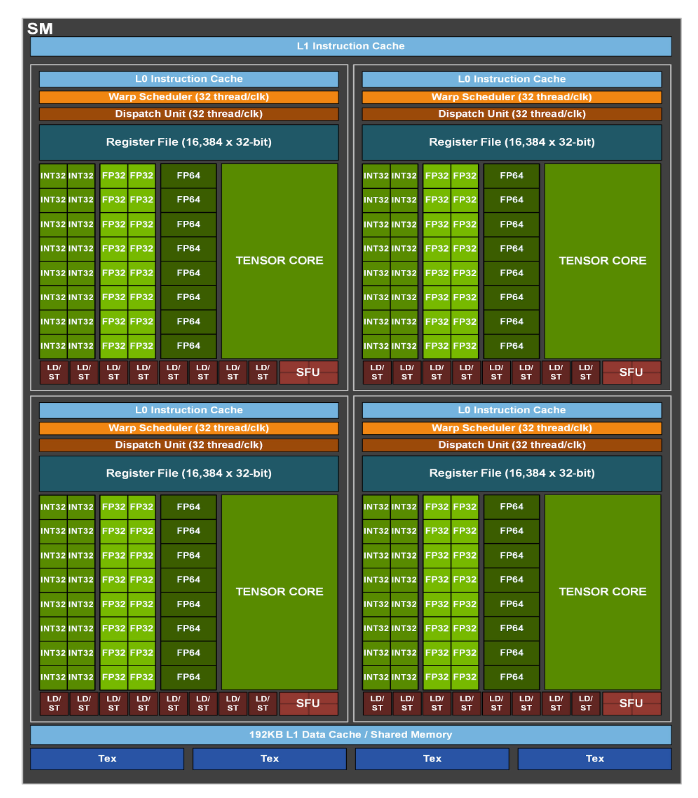
\includegraphics[scale=0.6]{./figure/volta_sm_arch.PNG}
\caption{Streaming Multiprocessor Architecture \cite{paper:41}}
\label{fig:voltasmarch}
\end{figure}

Composed of integer, FP32, FP64 units and the Tensor Core Units are designed specifically for deep learning. It introduces also new data types in the tensor core for the computation such as binary, integer 8 and 4 bits, floating-point 64, 32, 16 and bfp16 (the throughput of the tensor core computation for fp16 and bfp16 is the same). The Ampere SM can achieve such efficient workload on mixed computation and addressing calculations thanks to an independent parallel integer and floating-point data paths. \\\\

Matrix-Matrix multiplication operations are at the core of neural network training and inference, and are used to multiply large matrices of input data and weights in the connected layers of the network. The idea is represented into the Figure \ref{fig:tensorcorevolta} and compared to previous architectures.

\begin{figure}[!htbp]
\centering
\captionsetup{justification=centering}
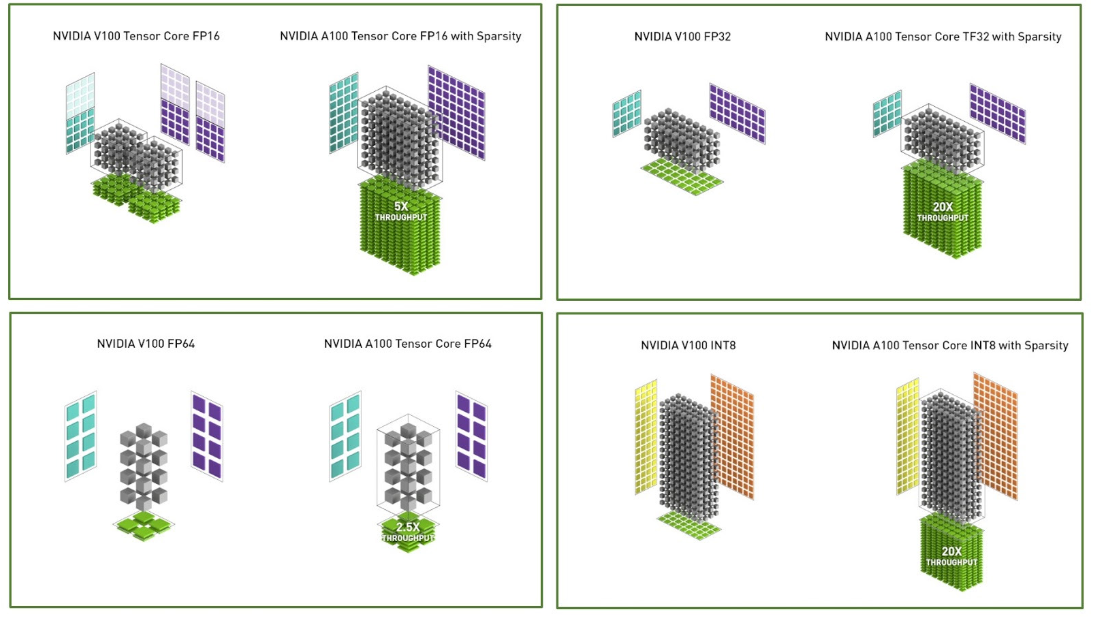
\includegraphics[scale=0.6]{./figure/tensor_core.PNG}
\caption{Matrix Multiplication in Tensor Core \cite{paper:41}}
\label{fig:tensorcorevolta}
\end{figure}

The Ampere A100 GPU contains 108 Streaming multiprocessor, and 432 third generation Tensor Core.
According to Figure \ref{fig:mixprec} the Tensor Core Units are able to compute multiplications on FP16 and accumulate on FP32, leading to a further reduction of latency and energy consumption.
\begin{figure}[!htbp]
\centering
\captionsetup{justification=centering}
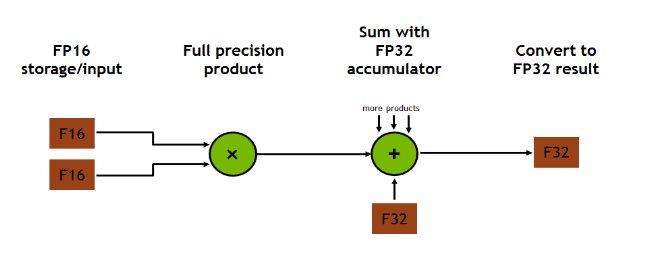
\includegraphics[scale=0.8]{./figure/mix_prec.PNG}
\caption{Mixed Precision Schema of a FMA unit in Tensor Core Unit \cite{paper:41}}
\label{fig:mixprec}
\end{figure}

A novel approach for doubling the throughput of deep neural networks has been introduced in this architecture. At the end of training process, only a subset of the total weights are necessary to execute a neural network correctly. As consequence not all the weights are needed, and they can be removed.\\
Based on training feedback, weights can be adapted at runtime during the training and this does not have any impact on the final accuracy. Thus, thanks to the sparsity of weight tensors., inference process can be accelerated. In addition, also the training process can be accelerated exploiting the sparsity idea but it has to be introduced at the beginning of the process for achieving some benefits.

\begin{figure}[!htbp]
\centering
\captionsetup{justification=centering}
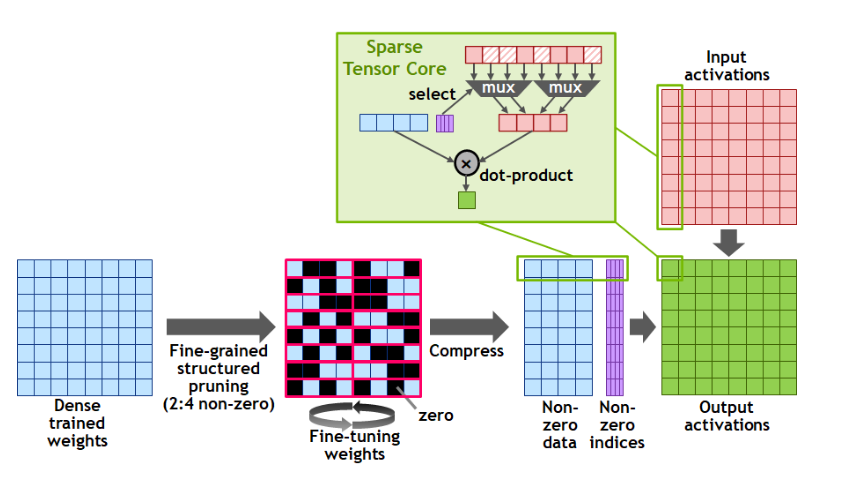
\includegraphics[scale=0.4]{./figure/sparsity.png}
\caption{Sparsity Optmization of a weight tensor \cite{paper:41}}
\label{fig:spa}
\end{figure}
The apporach in Figure \ref{fig:spa} doubles the throughput by skipping the zeros. It also leads to a reduction of memory footprint and an increase into the memory bandwidth.\\

Following the idea, NVIDIA has introduced a new set of instruction for inference: sparse Matrix Multiply-Accumulate (MMA). Those instructions are able to skip the matrix entries which contain zero values, leading to an increase of the Tensor core throughput. An example can be seen in Figure \ref{fig:mma}, where the light blue matrix has a sparsity of 50\%. It is also important to mention that the non-zero entries of the light blue matrix will be matched with the correct entries of the red one.
\begin{figure}[!htbp]
\centering
\captionsetup{justification=centering}
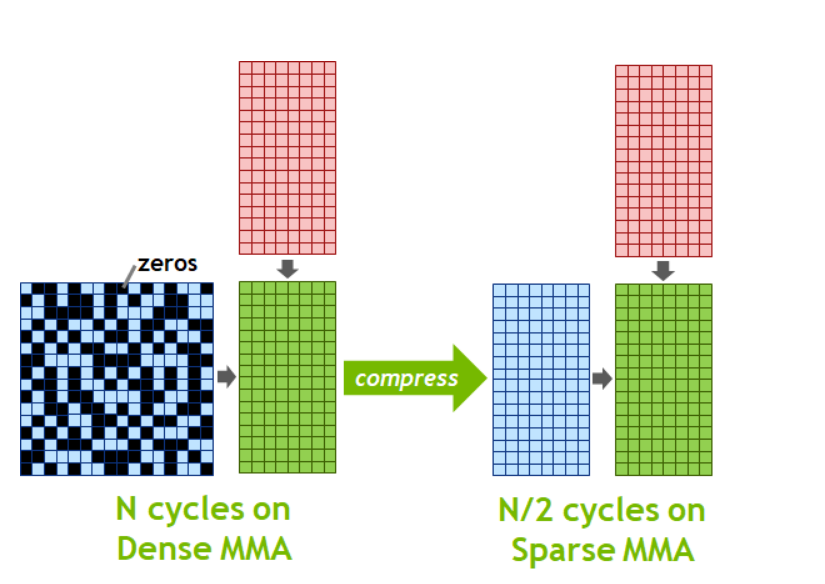
\includegraphics[scale=0.35]{./figure/mma.png}
\caption{Matrix Multiply Accumulate \cite{paper:41}}
\label{fig:mma}
\end{figure}

\newpage
The deep learning frameworks and the CUDA Toolkit include libraries that have been custom-tuned to provide high multi-GPU performance for each one of the following deep learning frameworks in the Figure \ref{fig:swtesla}.

\begin{figure}[!htbp]
\centering
\captionsetup{justification=centering}
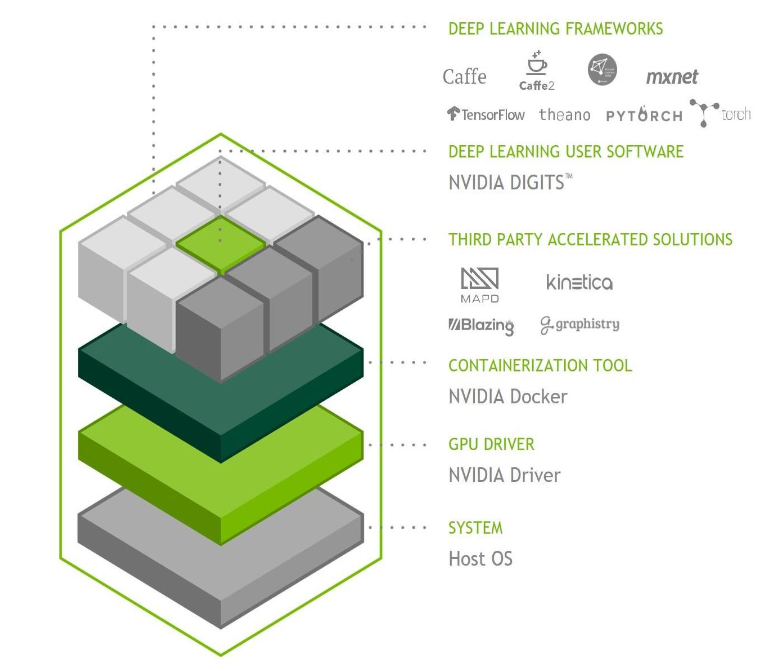
\includegraphics[scale=0.6]{./figure/sw_stack_tesla.PNG}
\caption{Software stack \cite{paper:41}}
\label{fig:swtesla}
\end{figure}

Combining powerful hardware with software tailored to deep learning, it provides to developers and researchers solutions for high-performance GPU-accelerated deep learning application development, testing, and network training.
\newpage
\section{Domain Specific Hardware Platform}
Instead of developing GPUs also suitable for Machine Learning applications, the companies have designed and deployed special purpose hardware accelerators.
\subsection{NVDLA}
The Nvidia Deep Learning Accelerator is a free open source hardware platform from Nvidia, highly customizable and modular, which allows to design and deploy deep learning inference hardware.

The architecture comes in two configurations:

\begin{figure}[!htbp]
\centering
\captionsetup{justification=centering}
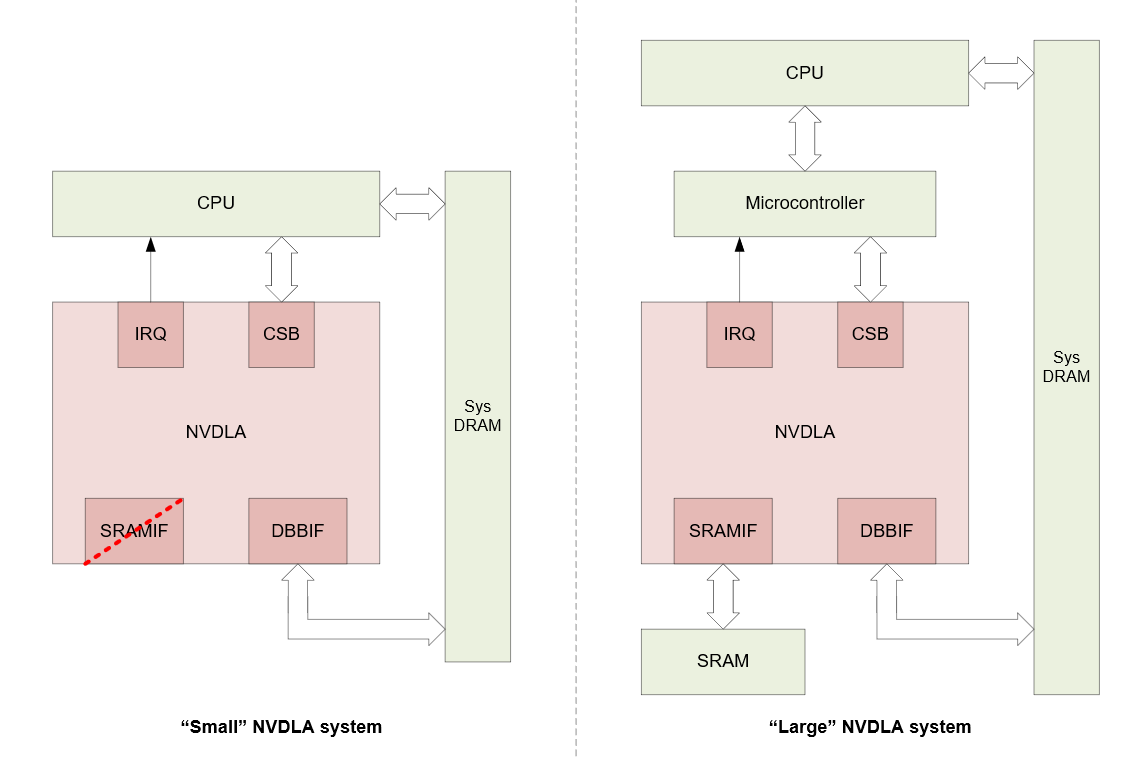
\includegraphics[scale=0.4]{./figure/nvdla_system.PNG}
\caption{Comparsion of two possible NVDLA system \cite{WEBSITE:8}}
\label{fig:nvdlasystem}
\end{figure}
As already mentioned, the aim of the work is to develop a hardware accelerator for machine learning suitable for mobile devices. Therefore from now on the NVDLA small system will be considered and analyzed.\\
The internal architecture of the NVDLA small system is:
\begin{figure}[!htbp]
\centering
\captionsetup{justification=centering}
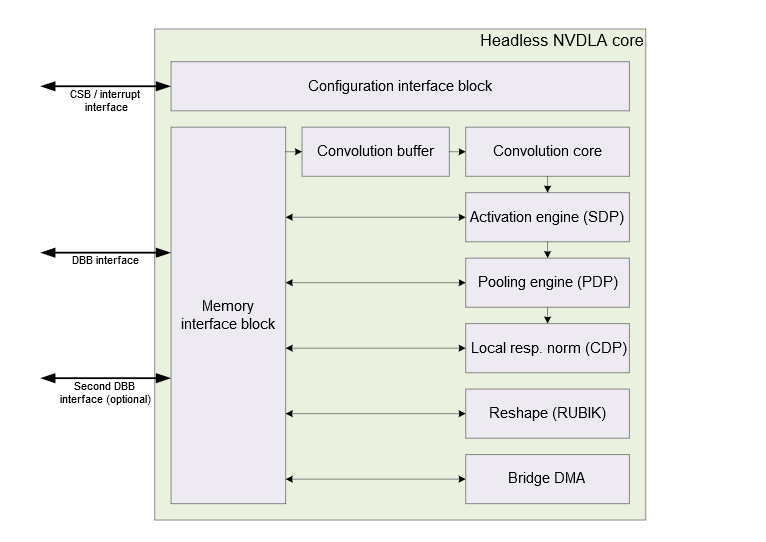
\includegraphics[scale=0.5]{./figure/nvdla_internal.PNG}
\centering\caption{Internal architecture of NVDLA small system, Secondary DBB not considered \cite{WEBSITE:8}}
\label{fig:nvdlaarch}
\end{figure}

According to Figure \ref{fig:nvdlasystem}, for the Small configuration of the accelerator, the processor will be in charge of programming and scheduling the operations on the NVDLA and as consequences handles the start/end of operations and possible interrupts, all of them through the CSB (Configuration Space Bus) interface which is AXI Lite compliant\cite{paper:30}. \newline
The data movement to/from memory are handled by the Internal memory controller through the DBB (Data BackBone) interface, which is AXI \cite{paper:30} compliant.\\

The internal architecture of NVDLA is composed by various engines. Each one of them is able to perform specific Machine Learning operations:
\begin{itemize}
\item Convolution Core: it comes in pair with the Convolution Buffer, its private memory for the data (inputs and weights). It is used to accelerate the convolution algorithms.
\item Activation engine (Single Data point Operations): it performs post processing operations at the single data element level such as bias addition, Non-linear function, PReLU (Parametric Rectified Linear Unit) and format conversion when the software requires different precision for different hardware layers.
\item Pooling engine (Planar Data Operations): it is designed to accomplish pooling layers, i.e. it executes operation along the width and height plane.
\item Local response normalization engine(Cross Channel Data operations): it is designed to address local response normalization layers.
\item Reshape(Data memory and reshape operations): it transforms data mapping format without any data calculation.
\item Bridge DMA: it is in charge of copying data from the Main Memory to the SRAM of the accelerator, only available into the large configuration of the system.
\end{itemize}

Another possible configuration which is worth to mention is the possibility to let the engines work separately on independent task or in a fused fashion where all of them are pipelined, working as a single entity.\\

According to developers the configurability of the cores ranges from arithmetic precision to the theoretical throughput that a single unit can achieve (increasing the number of internal Processing Elements). Moreover, since the engine units are independent of each other, according to the application and the model used they can be safely removed from the design.
\newpage
\subsubsection{ NVDLA Software }
It is also worth to mention that the accelerator comes already with a basic software stack:
\begin{figure}[H]
\centering
\captionsetup{justification=centering}
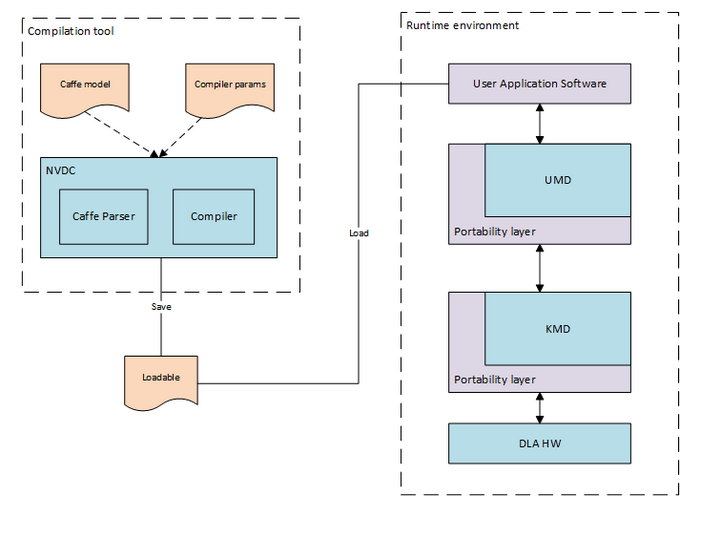
\includegraphics[scale=0.8]{./figure/nvdla_software.PNG}
\caption{NVDLA Software stack\cite{WEBSITE:7}}
\label{fig:nvdlasw}
\end{figure}

The Compilation tools are in charge of converting existing pretrained model into a set of hardware layers (for the desired precision) and programming sequences suitable for the NVDLA. The output of this process is a Nvidia Loadable file suitable for the runtime environment.\\
Regarding the runtime environment, it has been designed for a system in which is present an OS. It is composed in two parts: the User Mode Driver (UMD) and the Kernel Mode Driver (KMD).\newline The User Mode Driver loads the loadable file in memory and submits the operation to the KMD. It is also in charge of data movement from/to the accelerator. \newline The KMD is in charge of submitting operations to the accelerator through low level functions, scheduling the operations and handling the interrupts.\\
Both the KMD and the UMD are wrapped into portability layers which are, respectively, hardware dependent and OS dependent. In principle, for migrating the software to another OS or hardware plaftorm it is enough to modify only the portability layers.
\newpage
\subsection{Google TPU}
Google developed its own application-specific integragrated circuit for neural networks, which is tightly integrated with TensorFlow Software.
It includes:
\begin{itemize}
\item Matrix Multiplier Unit (MXU): 65,536 8-bit multiply-and-add units for matrix operations
\item Unified Buffer (UB): 24 MB of SRAM that work as registers
\item Activation Unit (AU): Hardwired activation functions
\end{itemize}

In Figure \ref{fig:tpuarch} a general view of TPU architecture is presented.
\begin{figure}[H]
\centering
\captionsetup{justification=centering}
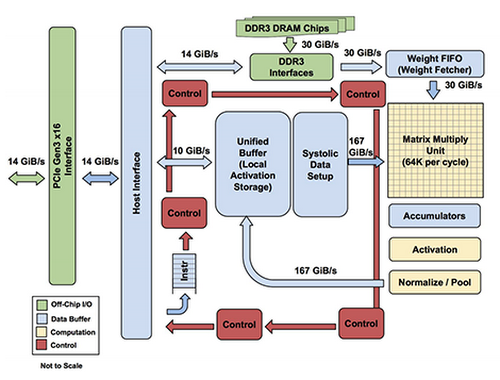
\includegraphics[scale=0.8]{./figure/tpu_arch.PNG}
\caption{Google TPU architecture\cite{paper:40}}
\label{fig:tpuarch}
\end{figure}

Rather than be tightly integrated with a CPU, the TPU is designed to be a coprocessor in which the instruction are sent by the host server rather than fetched.\\\\
The matrix multiplication unit reuses both inputs many times as part of producing the output, avoiding the overhead of continuously read data from memory. Only spatial adjacent ALU are connected together, which makes wires shorter and energy-efficient. The ALUs only perform computations in fixed pattern.
\newpage
As far as concerned the software stack, the TPU can be programmed for a wide variety of neural network models. To program it, API calls from TensorFlow graph are converted into TPU instructions.
\begin{figure}[H]
\centering
\captionsetup{justification=centering}
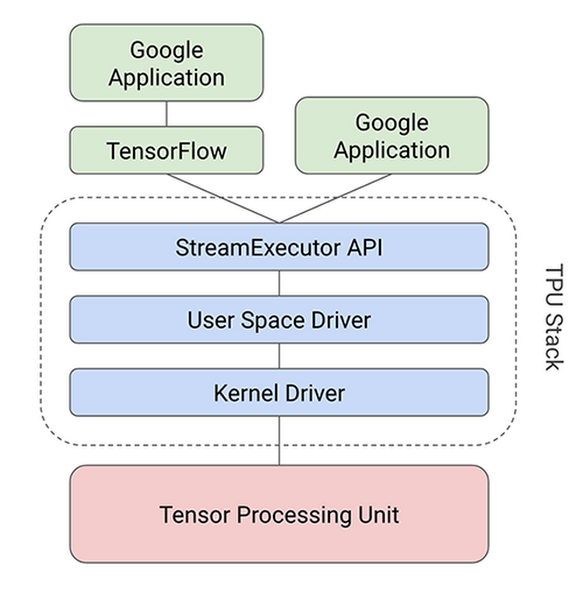
\includegraphics[scale=0.4]{./figure/tpu_sw_stack.PNG}
\caption{Google TPU Software Stack \cite{WEBSITE:9}}
\label{fig:gtpuswstack}
\end{figure}

\subsection{Habana Goya HL-1000}

Habana’s Goya is a processor dedicated to inference workloads. It is designed to deliver superior performance, power efficiency and cost savings for data centers and other emerging applications.\\
It allows the adoption of different deep learning models and is not limited to specific domains. Moreover, the performance requirements and accuracy can be user-defined.\\

In Figure \ref{fig:goyaarch} a high level view of the Goya architecture can be appreciated.
\begin{figure}[H]
\centering
\captionsetup{justification=centering}
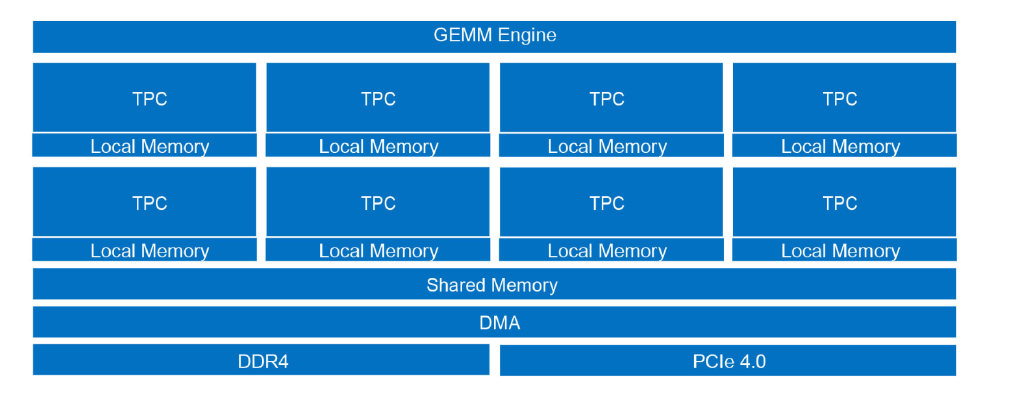
\includegraphics[scale=0.7]{./figure/goya_arch.PNG}
\caption{High level view of Goya architecture \cite{paper:38}}
\label{fig:goyaarch}
\end{figure}

It is based on scalable, fully programmable Tensor Processing Cores, specifically designed for deep learning workloads. \\
It also provides other flexible features such as GEMM operation acceleration, special functions dedicated hardware, tensor addressing, latency hiding capabilities and different data types support in TPC (FP32, INT32, INT16, INT8, UINT32, UINT16, UINT8).\\

Regarding the software stack, it can be interfaced with all deep learning frameworks. However, a model has to be first converted into an internal representation, as it can be seen in Figure \ref{fig:goyaswstack}.
\begin{figure}[H]
\centering
\captionsetup{justification=centering}
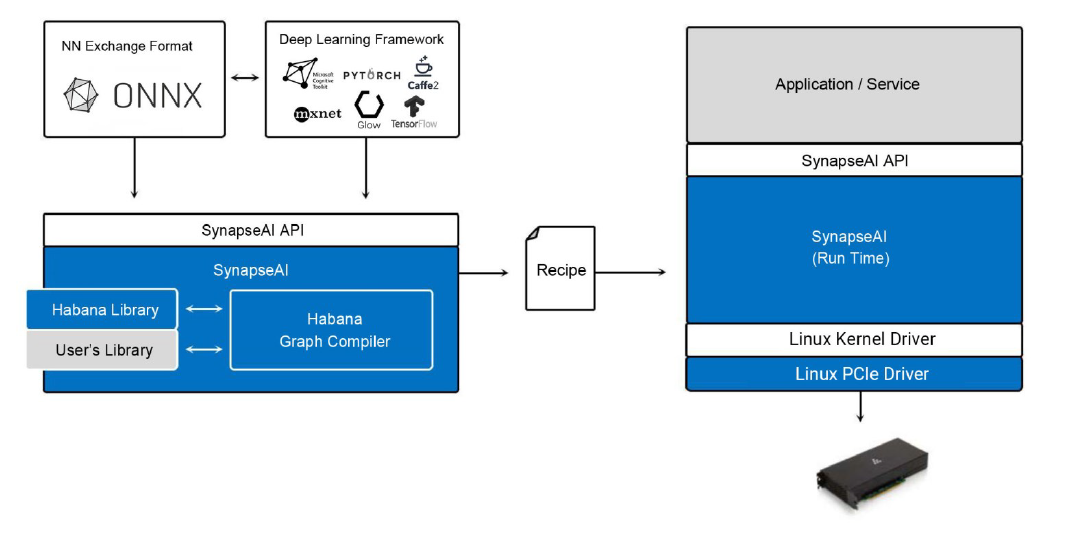
\includegraphics[scale=0.5]{./figure/goya_sw_stack.PNG}
\caption{Habana Goya Software Stack \cite{paper:38}}
\label{fig:goyaswstack}
\end{figure}
It also supports quantization of models trained in floating-point format with near-zero accuracy loss.

% METHODS

% CREATED BY DAVID FRISK, 2016
\chapter{System Devolopment}
\textit{In the following chapter a Top Down approach of the System development is described, with particular emphasis on the hardware development part.}
\section{Overview}
The entire work is implemented on a PYNQ Z2 board from TUL, based on a Zynq-7000 SoC \cite{paper:31}.

\begin{figure}[!htbp]
\centering
\captionsetup{justification=centering}
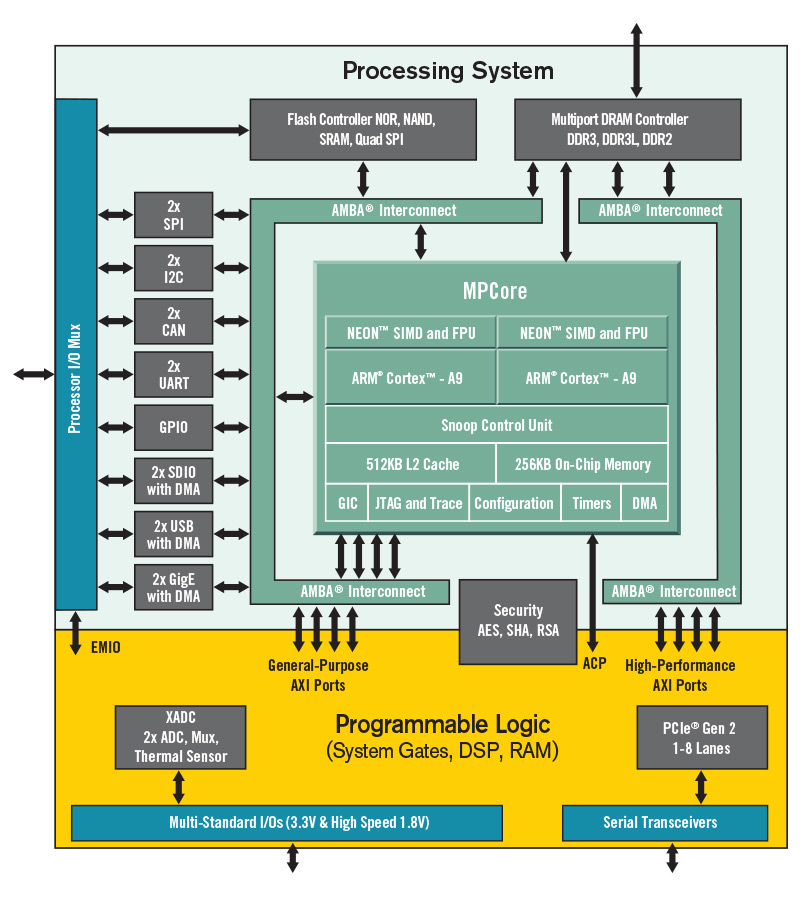
\includegraphics[scale=0.35]{./figure/zynq.PNG}
\caption{Zynq 7000 SoC}
\label{fig:zynq}
\end{figure}

The latter is composed of a programmable logic and a processing system, the Programmable logic hosts the accelerator and the relative AXI interconnections while the processing system is in charge of running the software for programming and scheduling correctly the operation on the accelerator.\newline In order to speed-up the development process and use built-in library for the AXI protocol and the DMA transfers, the software is carried out through the PYNQ enviroment of the board \cite{WEBSITE:2} which is based on Python. \\
The usage of Python as basic software allows to easily integrate it with high level Machine Learning API, such as TensorFlow in this case, an end-to-end open source Machine Learning platform \cite{WEBSITE:4}. It has the feature of quantize a post-trained model for different arithmetic precision.\\
Since the aim of the work is focused on the inference process, pre-trained models are needed and TensorFlow Hub \cite{WEBSITE:5} comes in handy for this purpose. It provides already pre-trained Machine Learning models for different domains.

\section{Software}
\todo[inline]{todo -> driver for accelerator and model from tensorflow (also offline quantization) }
\section{System Level}

As it can be seen from \ref{fig:zynq} , it is divided in two big block:
\begin{itemize}
\item Processing System:
The processing system in Figure \ref{fig:sys} referred as \textit{ps7} is in charge of running the OS and the Machine Learning application, as consequence it also runs the necessary software for programming the accelerator registers and the data movement to/from main memory from/to the accelerator.
\item Programmable Logic:
The programmable logic (PL) hosts the entire design, from the accelerator itself to the DMAs and the AXI interconnections.\\ Several single channel DMA have been used instead of using a single DMA with multiple channels, the reason is that the in the PYNQ enviroment only the drivers for the single channel DMA are provided. Furthermore, the Programmable Logic can be divided into:
\begin{itemize}
\item AXI interconnections: IP cores from Xilinx\cite{paper:34}\cite{paper:35} in order to connect and correctly address entities in the Programmable Logic.
\item AXI DMA: IP core from Xilinx \cite{paper:33} which allows data movement between main memory and accelerator memories.
\item DTPU: the actual hardware accelerator.
\item XADC: IP core from Xilinx \cite{paper:32} which allows to measure the temperature of the SoC, the voltages and the currents at runtime.

\end{itemize}

\end{itemize}

\newpage
In the following figure, the schematic of the overall design is presented.
\begin{figure}[!htbp]
\centering
\captionsetup{justification=centering}
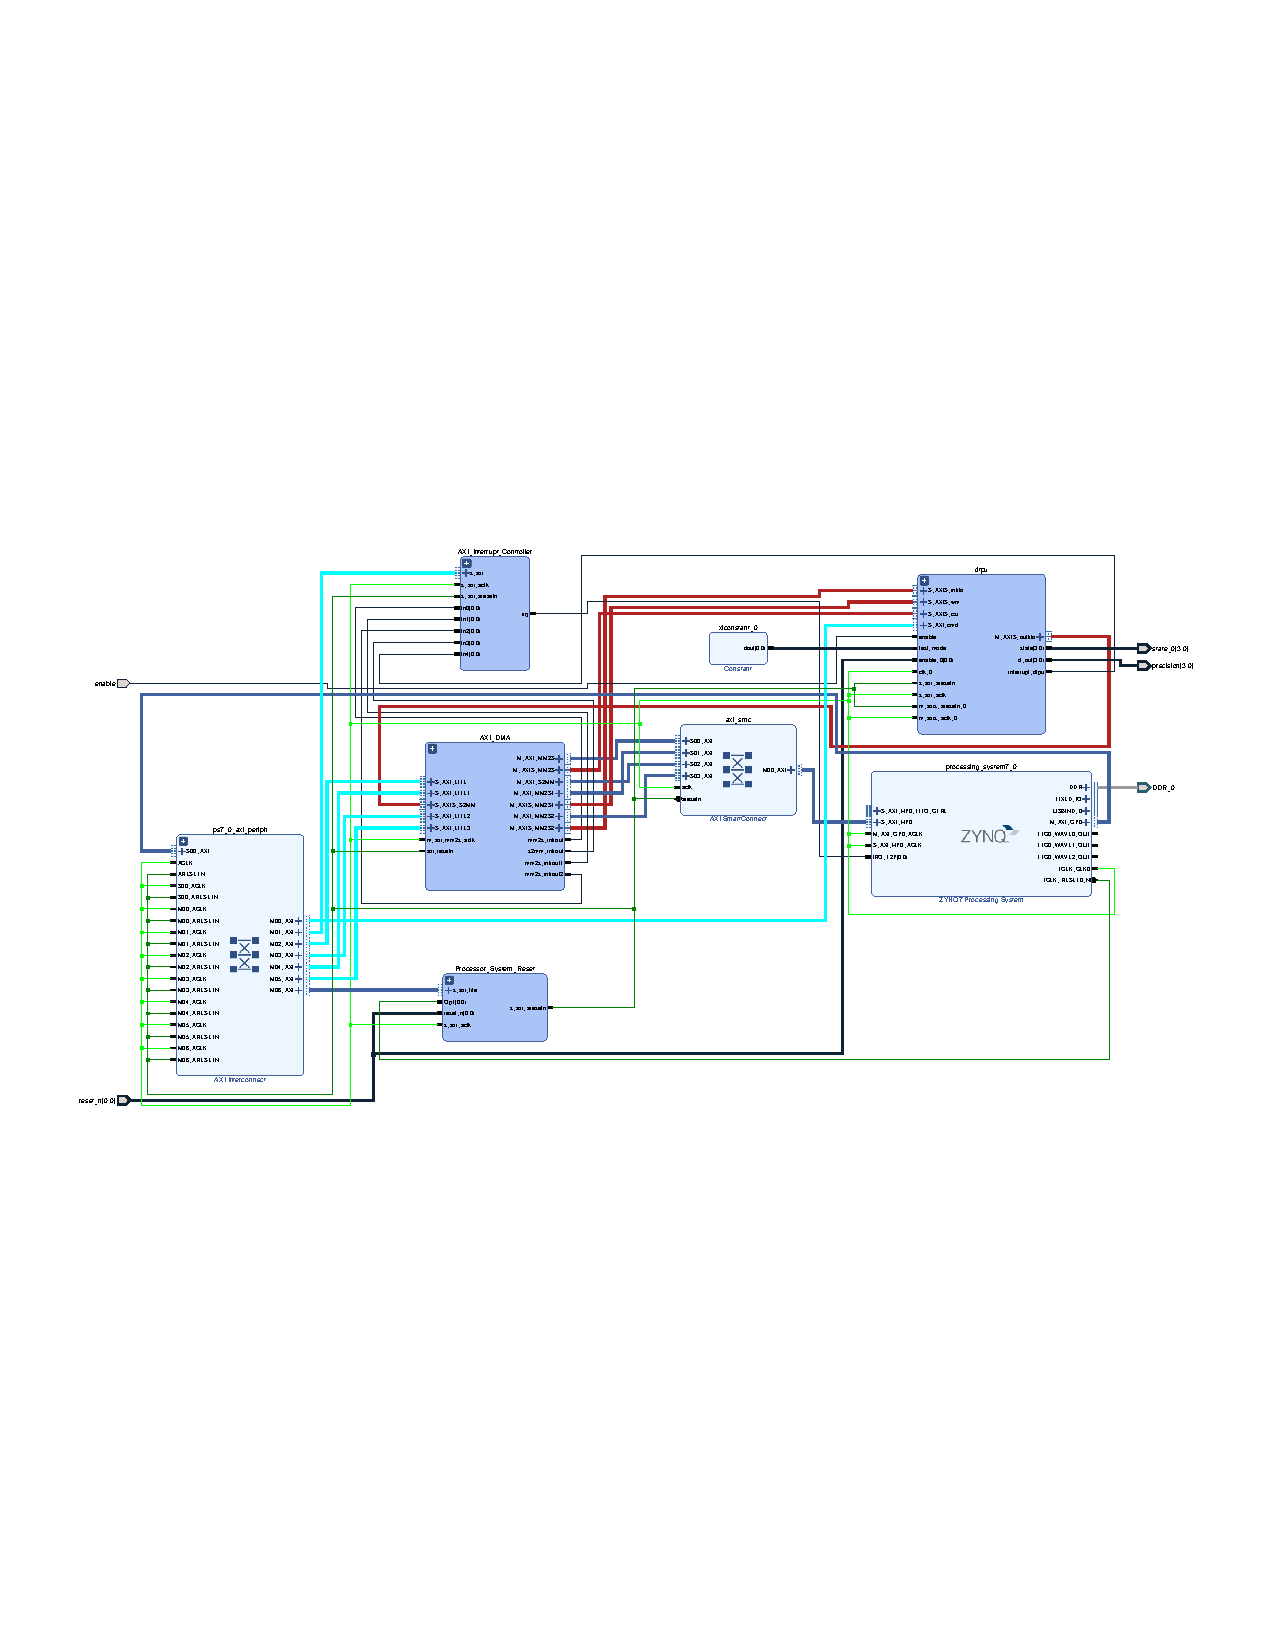
\includegraphics[scale=0.97,angle=90]{./figure/system_schematic.pdf}
\caption{System}
\label{fig:sys}
\end{figure}

\section{DTPU the hardware accelerator}

\subsection{Overview}
\todo[inline]{schematic}

\subsection{Real Implementation}
\todo[inline]{schematic from vivado }
\subsubsection{Axi accelerator adapter}
\subsubsection{DTPU core}


% RESULTS
% CREATED BY DAVID FRISK, 2016
\chapter{Results}

\epigraph{ \textit{If you can not measure something, you can not improve it.}}{--- \textup{William Thomson Kelvin}}

\section{Evaluation metrics}
Generally speaking in Computer Science, every domain and application could have different evaluation metrics, for example the energy efficient of a CPU is a heavy metrics in embedded systems while in a high performant CPU latency and throughput are dominant metrics. As said that, evaluation metrics strongly depend on the end-users, therefore the designers have to make assumption on the end-user intentions and applications.\\
In this work the assumptions are that the accelerator will be deployed into an embedded system and at the same time it should give to the user a certain degree of flexibility for running Neural Network models. Thus, as it is suggested \cite{paper:1} the following metrics are used:
\begin{itemize}
\item Accuracy, quality of the final result of inference process.
\item Throughput, for measuring real time performance. It depends on the number of internal computation cores.
\item Latency, for interactive applications.
\item Energy and Power.
\item Hardware cost (Utilization Factor in case of an FPGA) of chip area and process technology.
\end{itemize}
\newpage
\section{Utilization Factor}
An important aspect of an embedded system is the on-die utilization area. Those kinds of system are usually deployed on tight area-constrained chips for hiding their presence to the user.
Therefore, it is important to measure and understand the behavior on the Utilization of the FPGA (used as area measurement in this case) of the design as the size of Matrix Multiplication Unit increases and in parallel the throughput.\\
The Utilization Factor, composed of Look-up-Table, Flip Flops and Digital Signal Processor usage, is expected to increase as the size of Multiplication Matrix increase and the bit width of Computation Unit.\\
In the following Figures, utilization results are presented for each data type, where the Matrix Multiplication Unit sizes are pushed as much as the timing requirements are meet:
\begin{itemize}
\item Integer 8 bit:
\begin{figure}[!htbp]
\centering
\captionsetup{justification=centering}
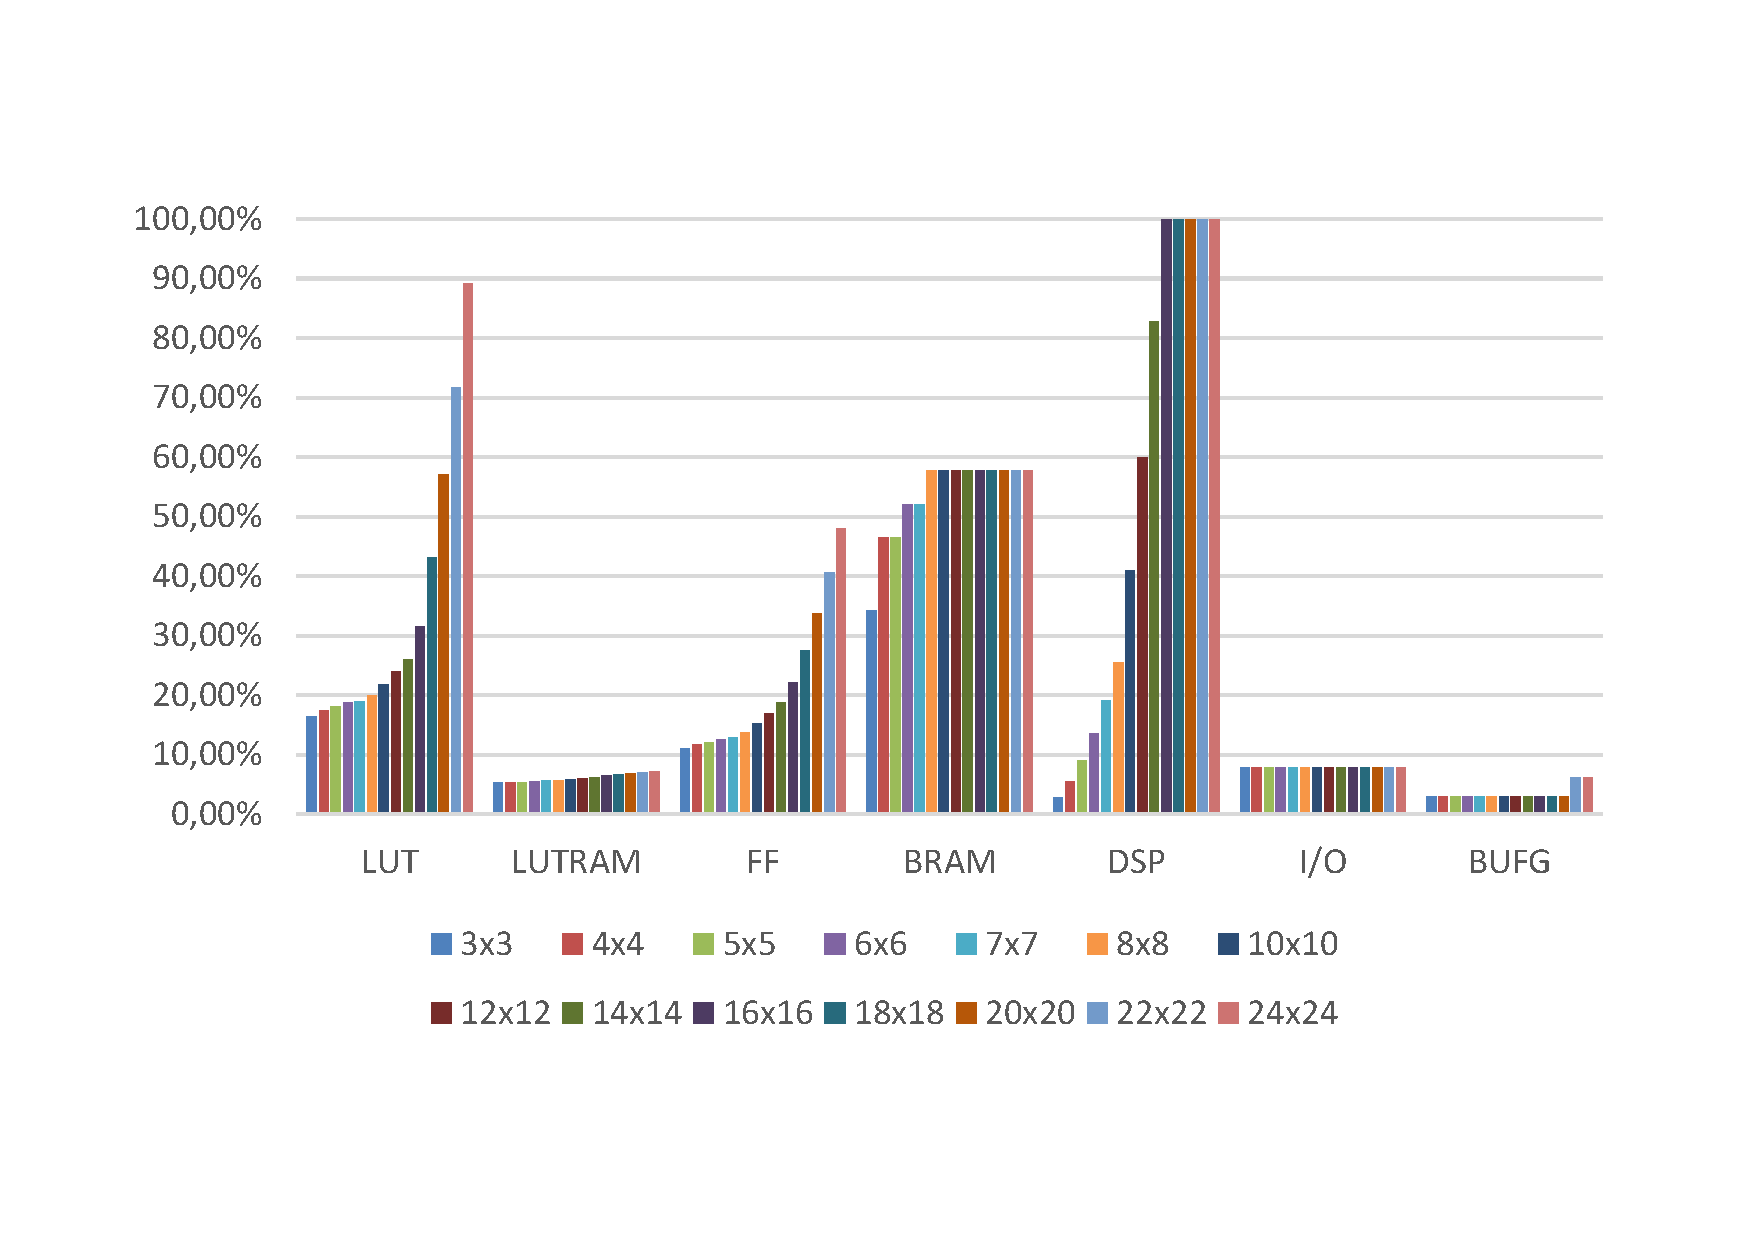
\includegraphics[scale=0.35,angle=0]{./figure/graphs/utilization_factor_30mhz_int8.pdf}
\caption{Post Implementation Utilization Factor of integer 8 bit PEs and clock frequency of 30 Mhz}
\label{fig:ut8bit}
\end{figure}
\item Integer 16 bit:
\begin{figure}[!htbp]
\centering
\captionsetup{justification=centering}
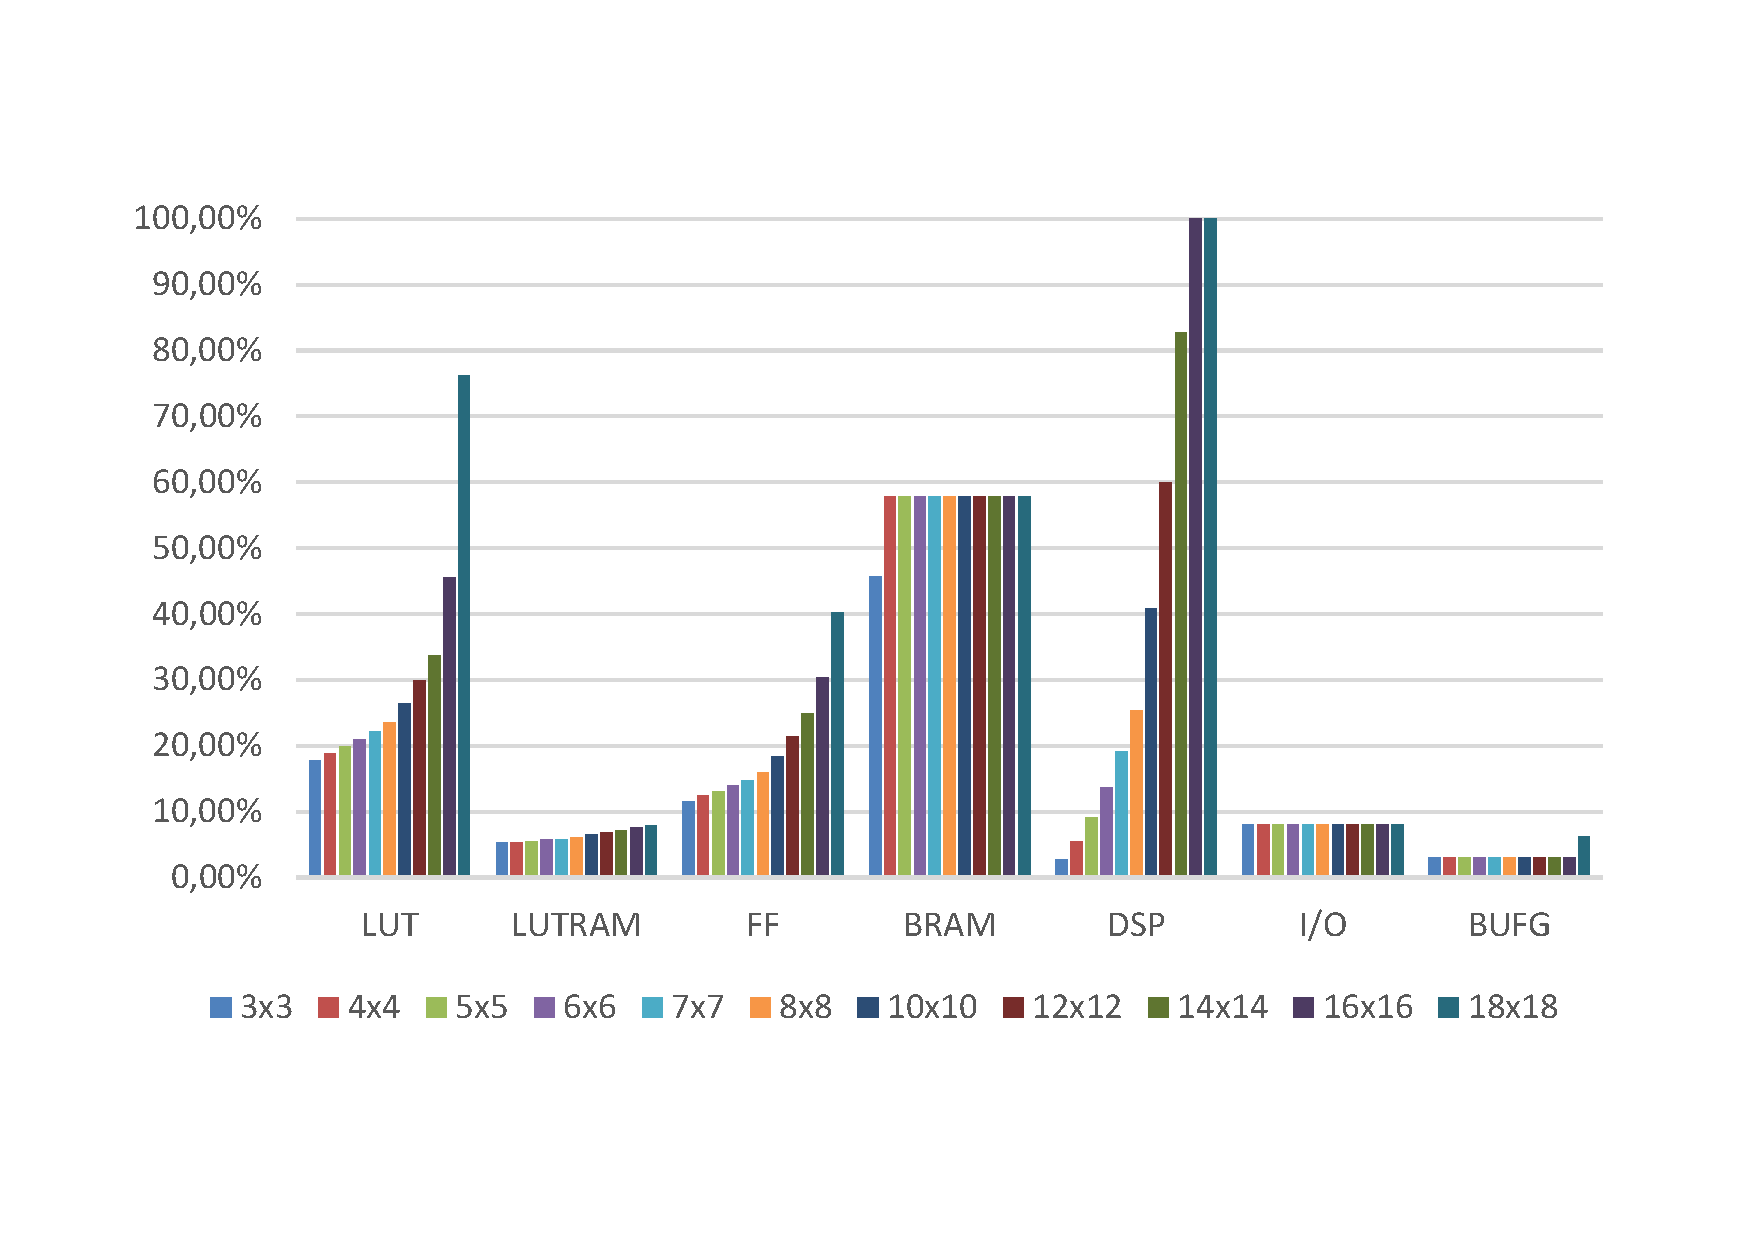
\includegraphics[scale=0.35,angle=0]{./figure/graphs/utilization_factor_30mhz_int16.pdf}
\caption{Post Implementation Utilization Factor of integer 16 bit PEs and clock frequency of 30 Mhz}
\label{fig:ut16bit}
\end{figure}
\newpage
\item Integer 32 bit:
\begin{figure}[!htbp]
\centering
\captionsetup{justification=centering}
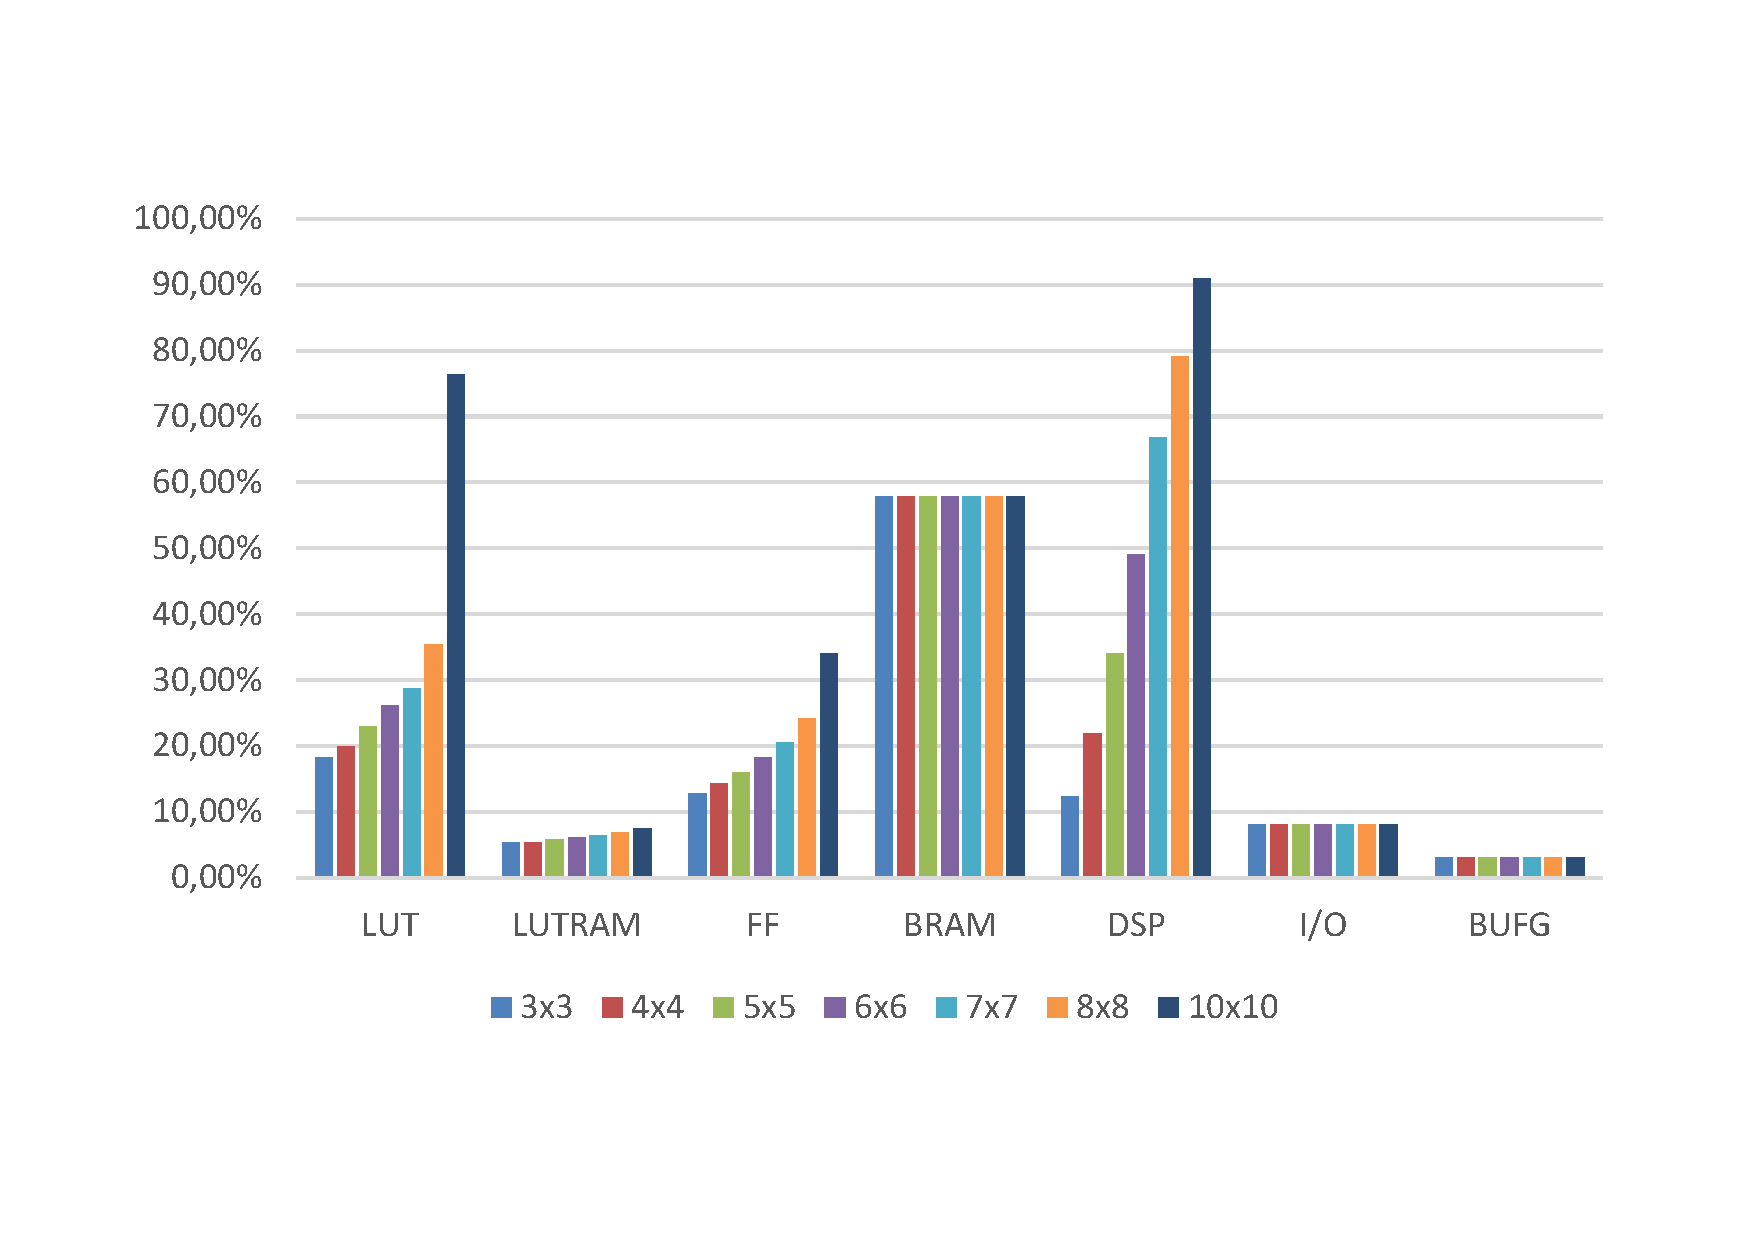
\includegraphics[scale=0.35,angle=0]{./figure/graphs/utilization_factor_30mhz_int32.pdf}
\caption{Post Implementation Utilization Factor of integer 32 bit PEs and clock frequency of 30 Mhz}
\label{fig:ut32bit}
\end{figure}
\item Integer 64 bit:
\begin{figure}[!htbp]
\centering
\captionsetup{justification=centering}
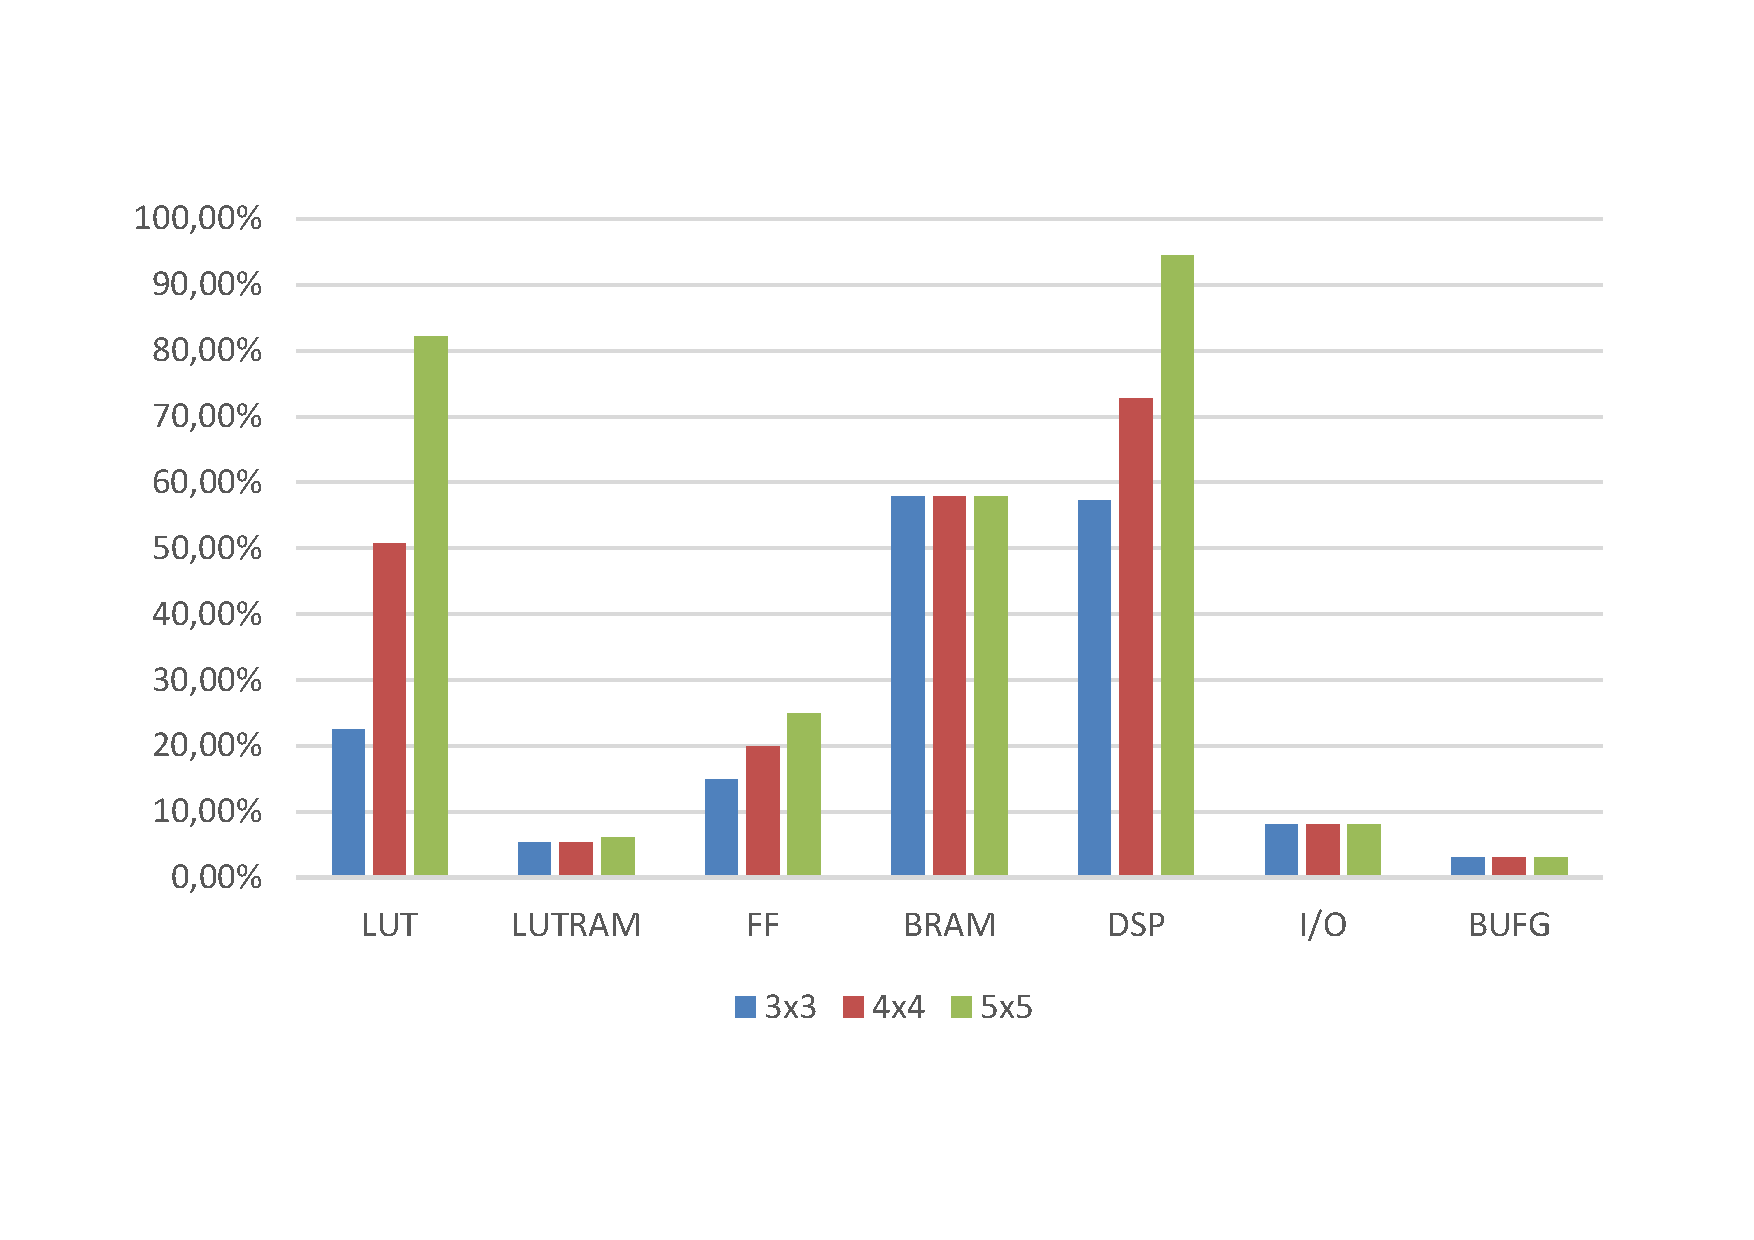
\includegraphics[scale=0.35,angle=0]{./figure/graphs/utilization_factor_30mhz_int64.pdf}
\caption{Post Implementation Utilization Factor of integer 64 bit PEs and clock frequency of 30 Mhz}
\label{fig:ut64bit}
\end{figure}
\item Brain Floating point 16:
\begin{figure}[!htbp]
\centering
\captionsetup{justification=centering}
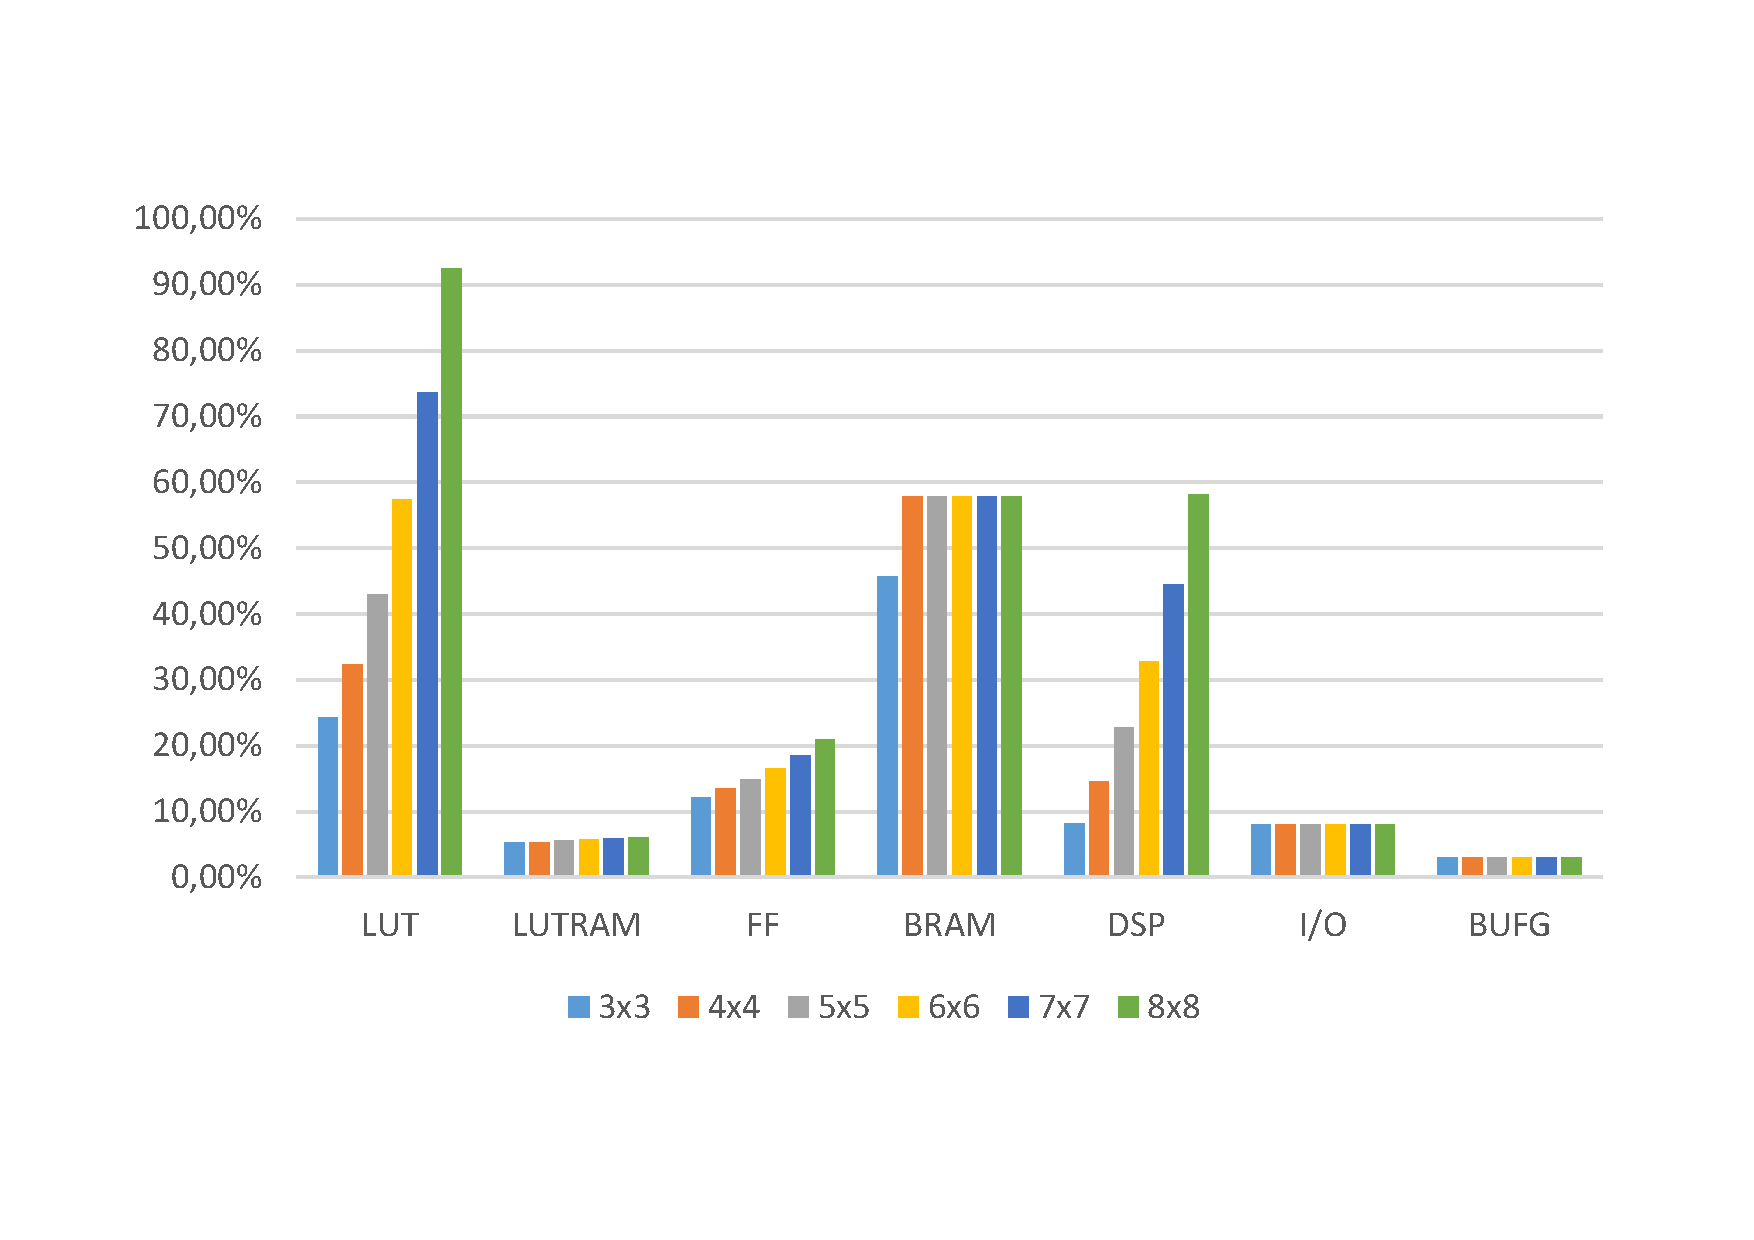
\includegraphics[scale=0.35,angle=0]{./figure/graphs/utilization_factor_30mhz_bfp16.pdf}
\caption{Post Implementation Utilization Factor of bfp 16 bit PEs and clock frequency of 30 Mhz}
\label{fig:utbpf16bit}
\end{figure}
\newpage
\item Floating point 32:
\begin{figure}[!htbp]
\centering
\captionsetup{justification=centering}
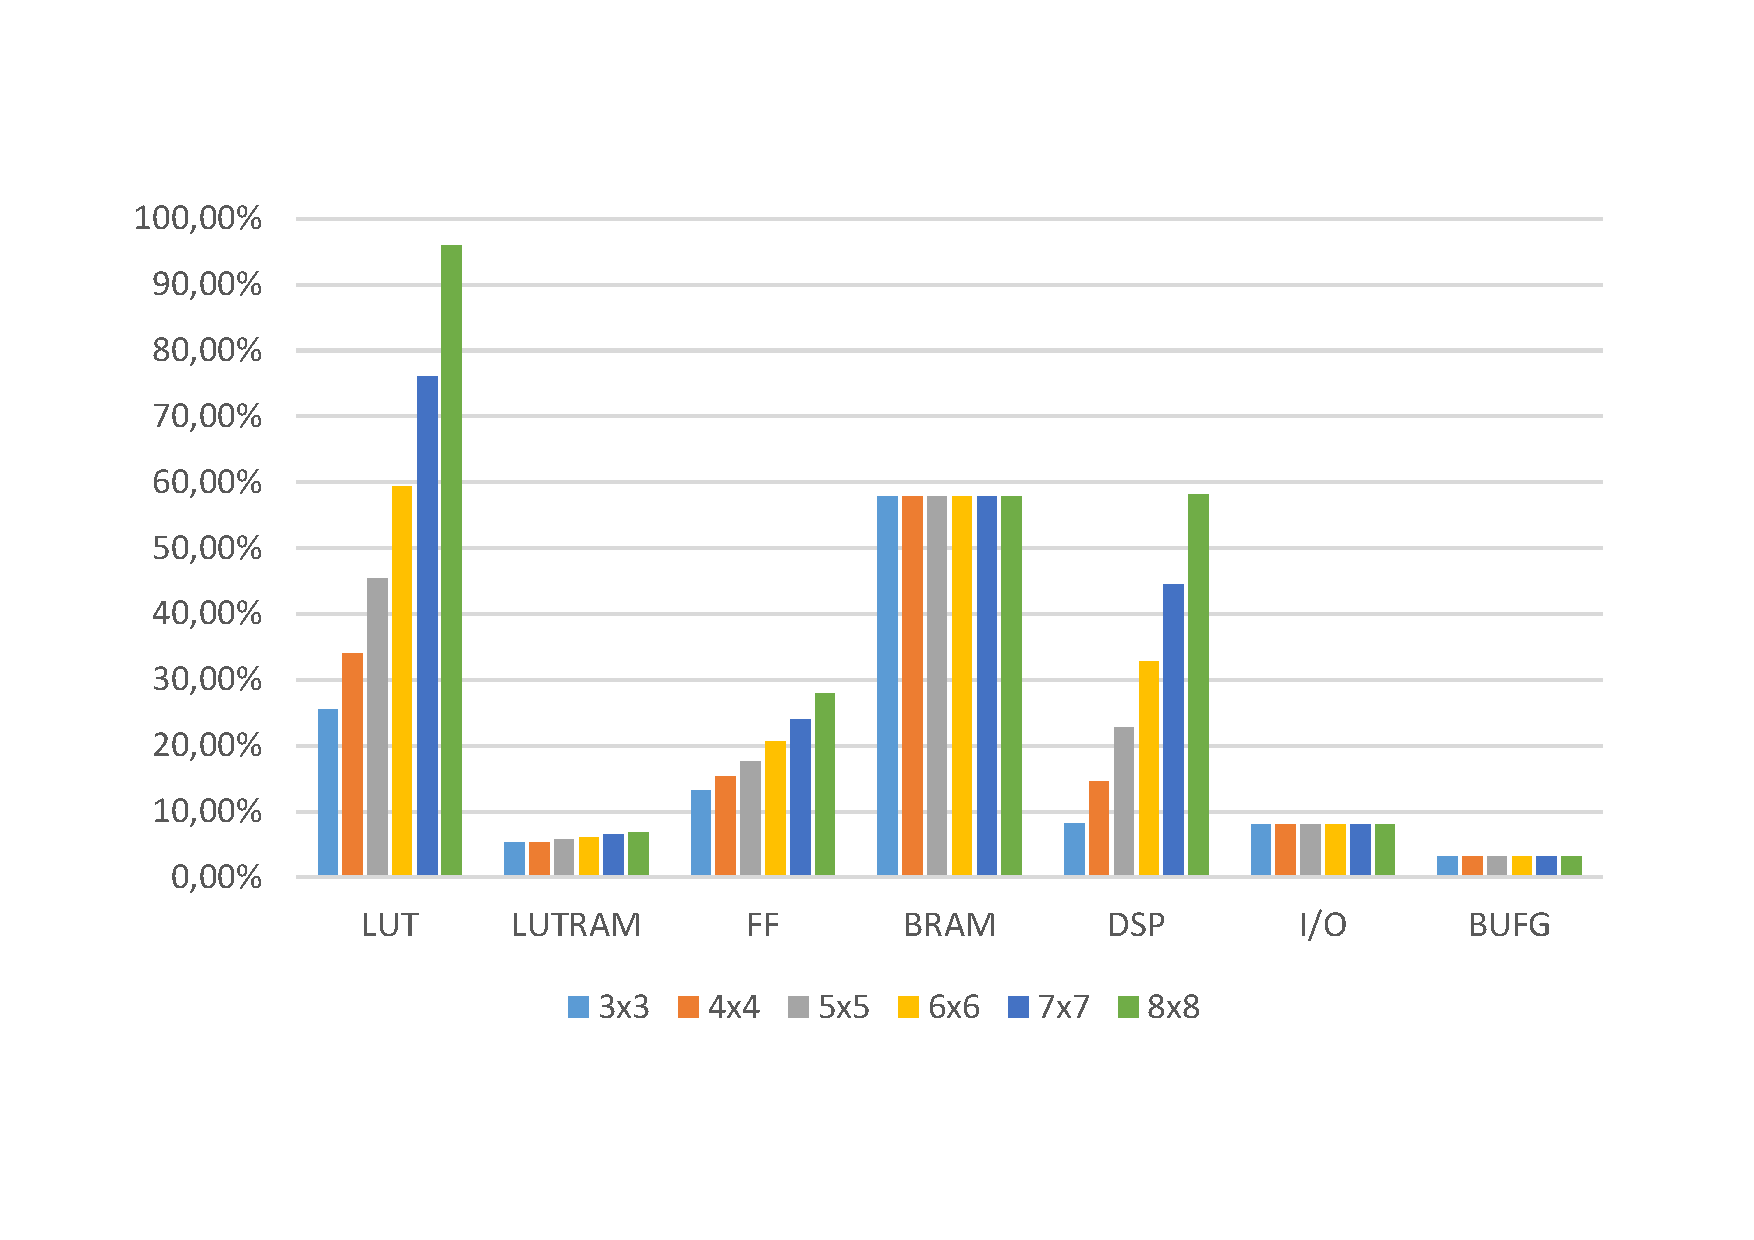
\includegraphics[scale=0.35,angle=0]{./figure/graphs/utilization_factor_30mhz_fp32.pdf}
\caption{Post Implementation Utilization Factor of fp 32 bit PEs and clock frequency of 30 Mhz}
\label{fig:utfp32bit}
\end{figure}
\end{itemize}
It can be seen that the trend for integer 8 and 16 is similar (Figure \ref{fig:ut8bit} and \ref{fig:ut16bit}). It is a 1 to 1 mapping between the PE and the DSP entity on the board. Actually, the DSP entities are on 16 bit and using the 8 bit units the high 8 bits are gated to zeros.\\ 
As soon as the DSP are used the utilization of LUT and FF is linear in the sizes of Matrix Multiplication unit, while the DSP utilization is quadratic. At a full utilization of DSP entities the PEs start to be implemented in logic and it can be seen, in all the previous graphs, a sudden rise in the LUT utilization.\\It is also worth to mention that the PEs on 64 bit integer are a special case of FPGA's utilization, they reach sooner than the other designs the full utilization. Every PEs in this configuration is using a 14 DSP entities for taking into account also the possibility of computing vectorized operations as previously mentioned.\\\\
Regarding the floating point units, it has been used the same hardware unit for both the fp32 and bfp16, since they have the same exponent bit length but different mantissa length (this also allows to have the same numerical stability). Relying on the synthesis process to properly optimize the different units and discard, where necessary, the unused hardware. In fact, comparing Figure \ref{fig:utbpf16bit} with Figure \ref{fig:utfp32bit}, there is a slight different in the utilization of the LUT and a more remarkable difference in FF utilization.\\

Increasing the clock frequency, the FPGA's utilization is reduced since with an increase of the Matrix Multiplication Unit sizes the design is not able anymore to meet the timing requirements, especially for the floating point units. 
\newpage

\section{Energy and Power Consumption}
Energy and Power consumption are important factor, for a mobile device in which there is a limited battery capacity meanwhile for data centers stringent power ceilings due to cooling costs.\\ 
According to the Vivado Power estimation manual\cite{paper:49}, the static power is calculated over all the FPGA resources. This is due to the hard estimation of the static power per single design.
In the following Figures, estimations of power consumption from Vivado are presented for each data type and different clock frequencies:
\begin{itemize}
\item Integer 8:
\begin{figure}[!htbp]
\centering
\captionsetup{justification=centering}
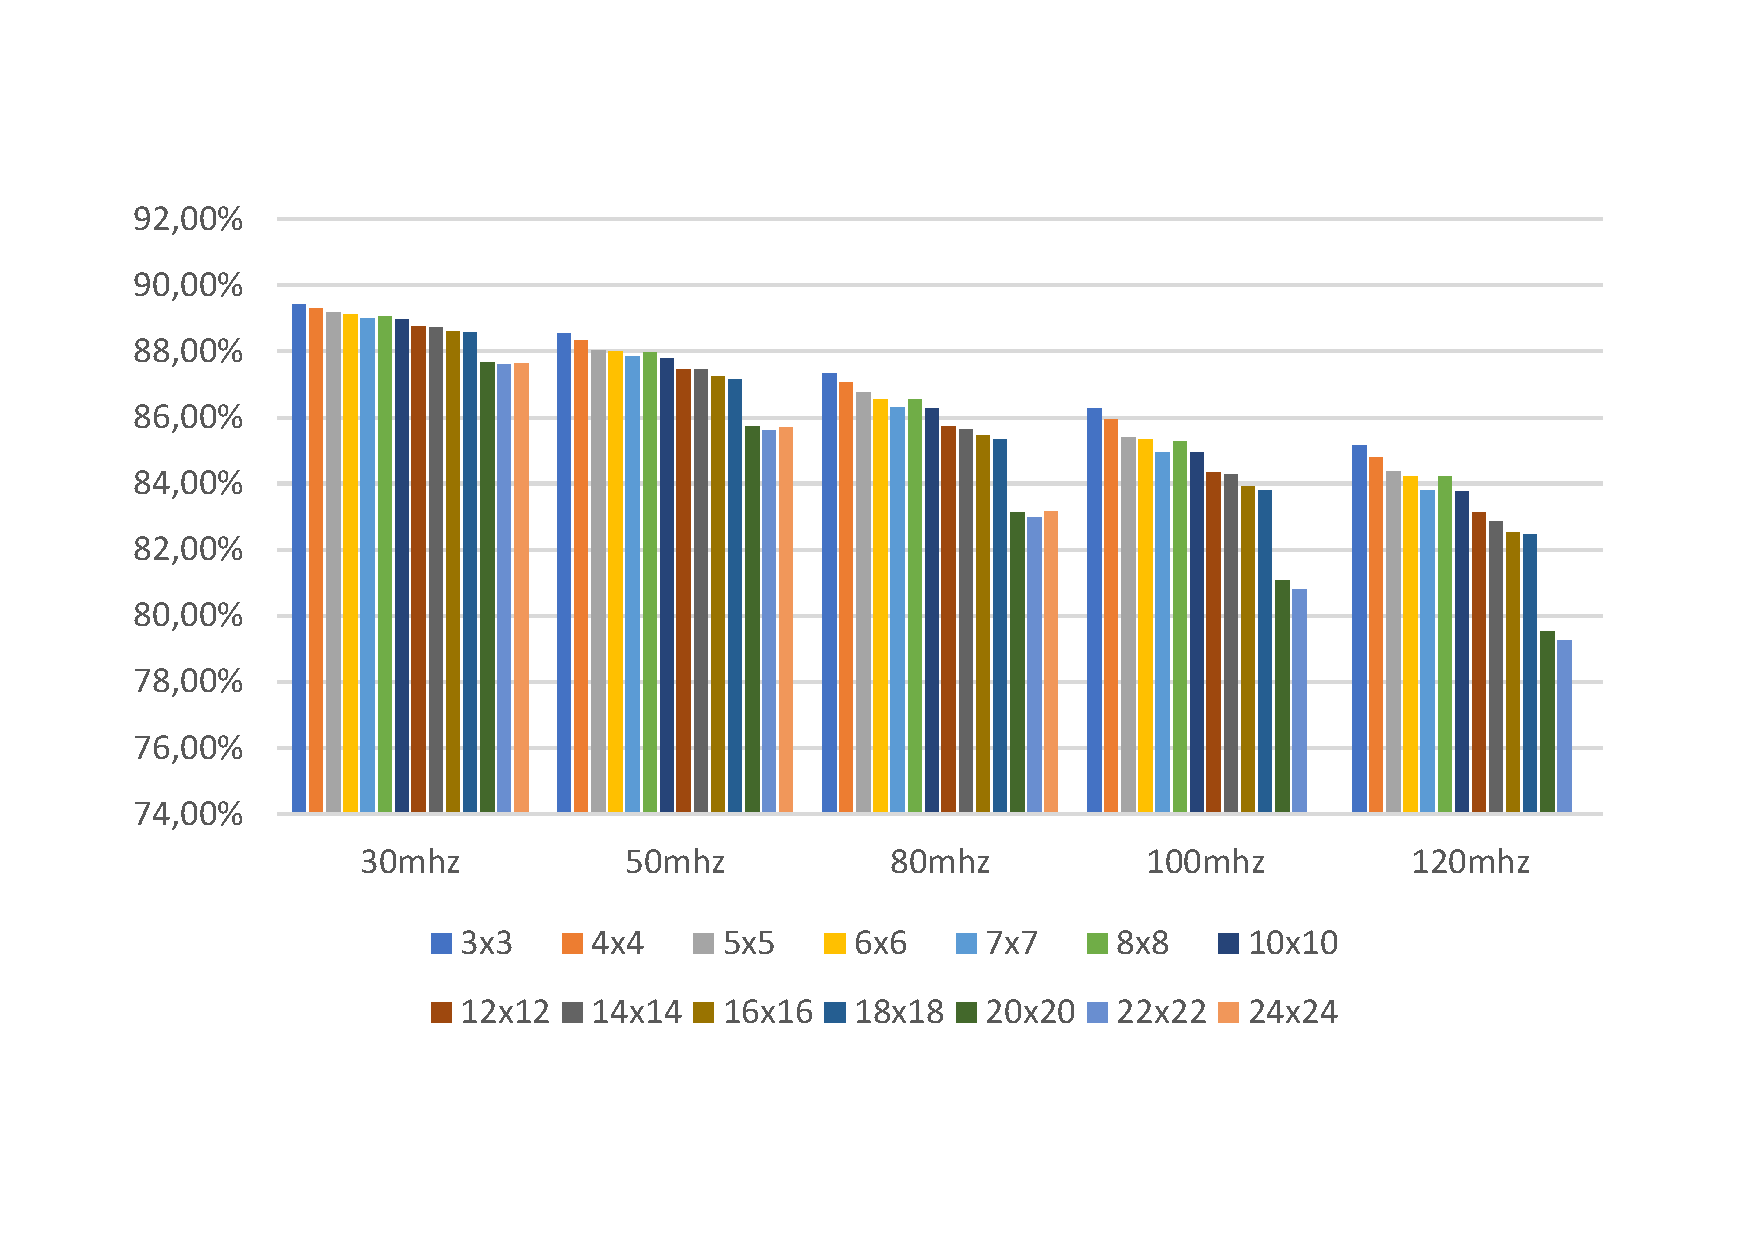
\includegraphics[scale=0.45,angle=0]{./figure/graphs/power_ps_int8_freq.pdf}
\caption{Post Implementation Power Consumption of Processing System for integer 8 PEs}
\label{fig:powint8}
\end{figure}
\begin{figure}[!htbp]
\centering
\captionsetup{justification=centering}
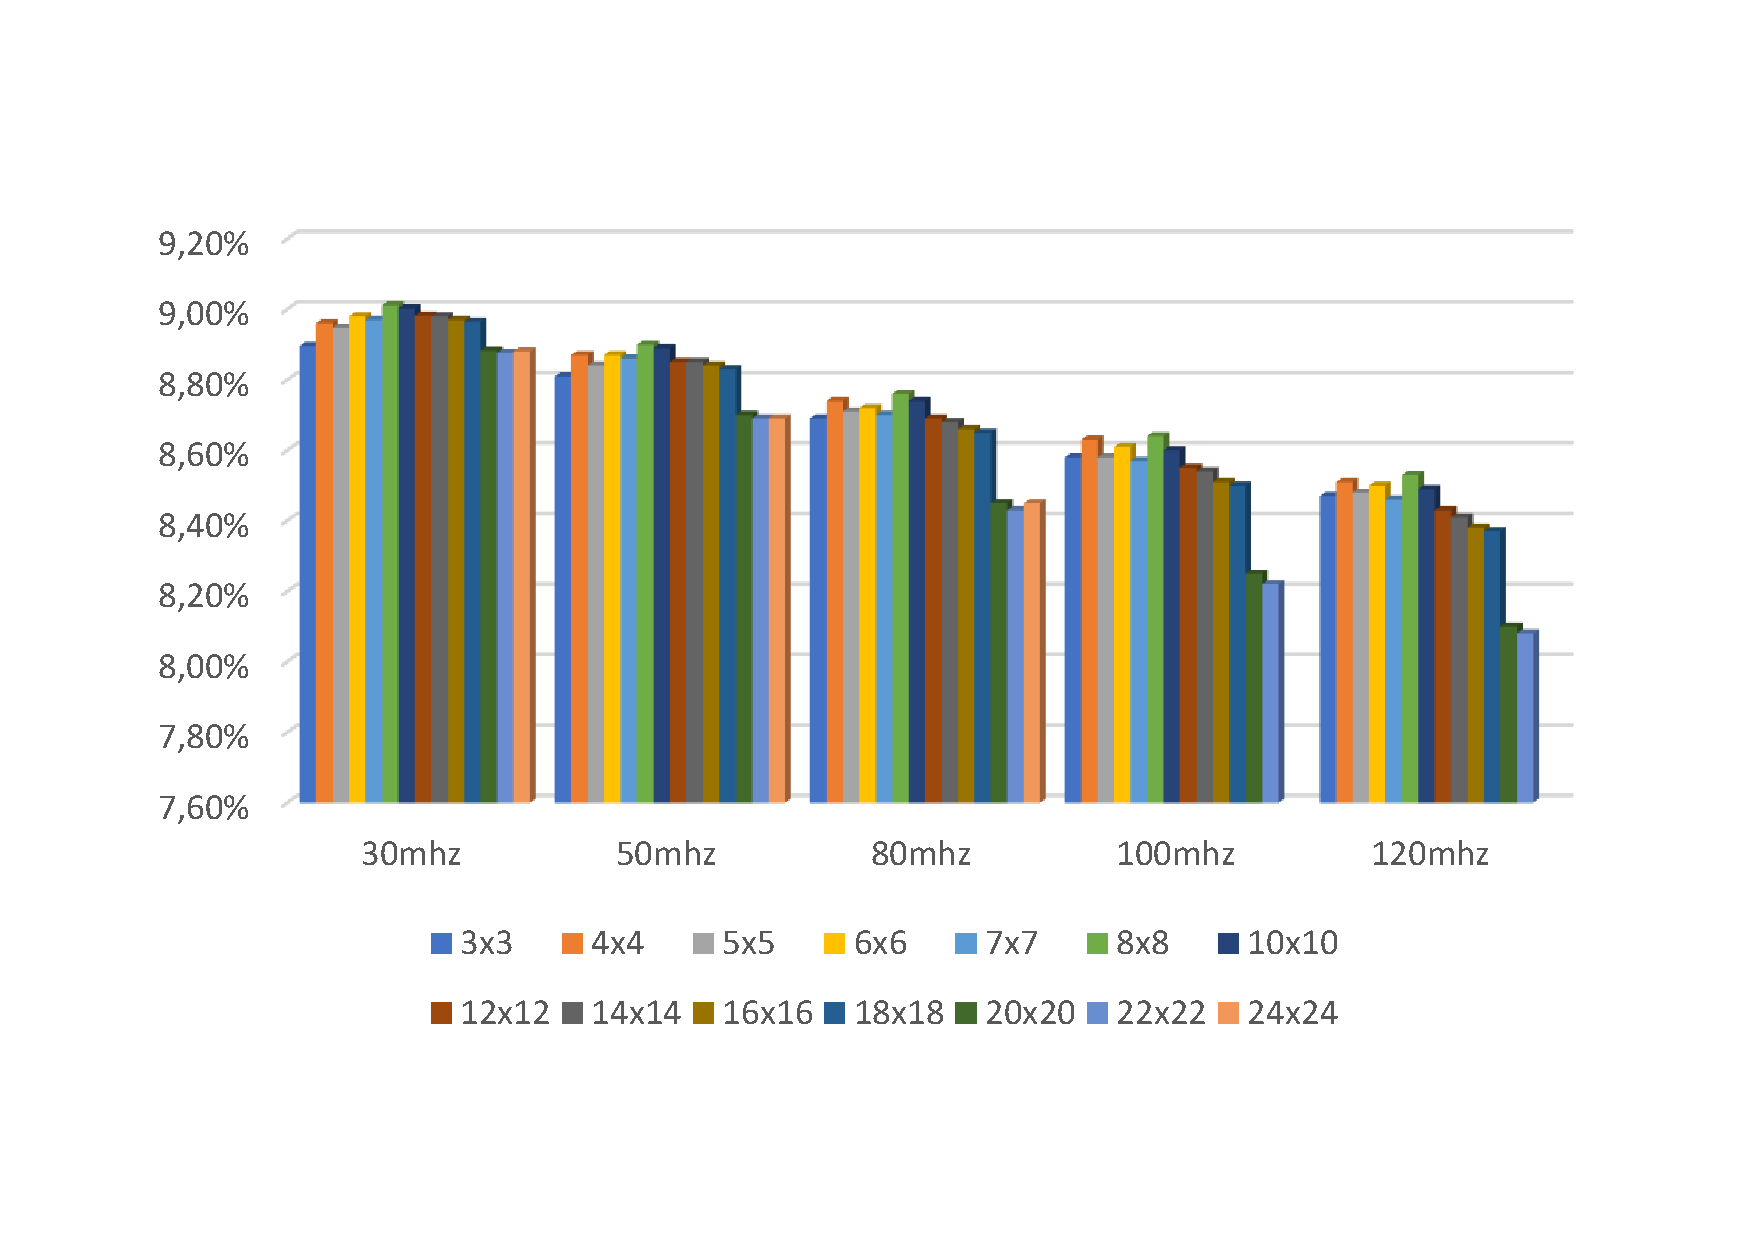
\includegraphics[scale=0.45,angle=0]{./figure/graphs/power_plstatic_int8_freq.pdf}
\caption{Post Implementation Static Power Consumption Programmable logic for integer 8 PEs }
\label{fig:staticpowint8}
\end{figure}
\begin{figure}[!htbp]
\centering
\captionsetup{justification=centering}
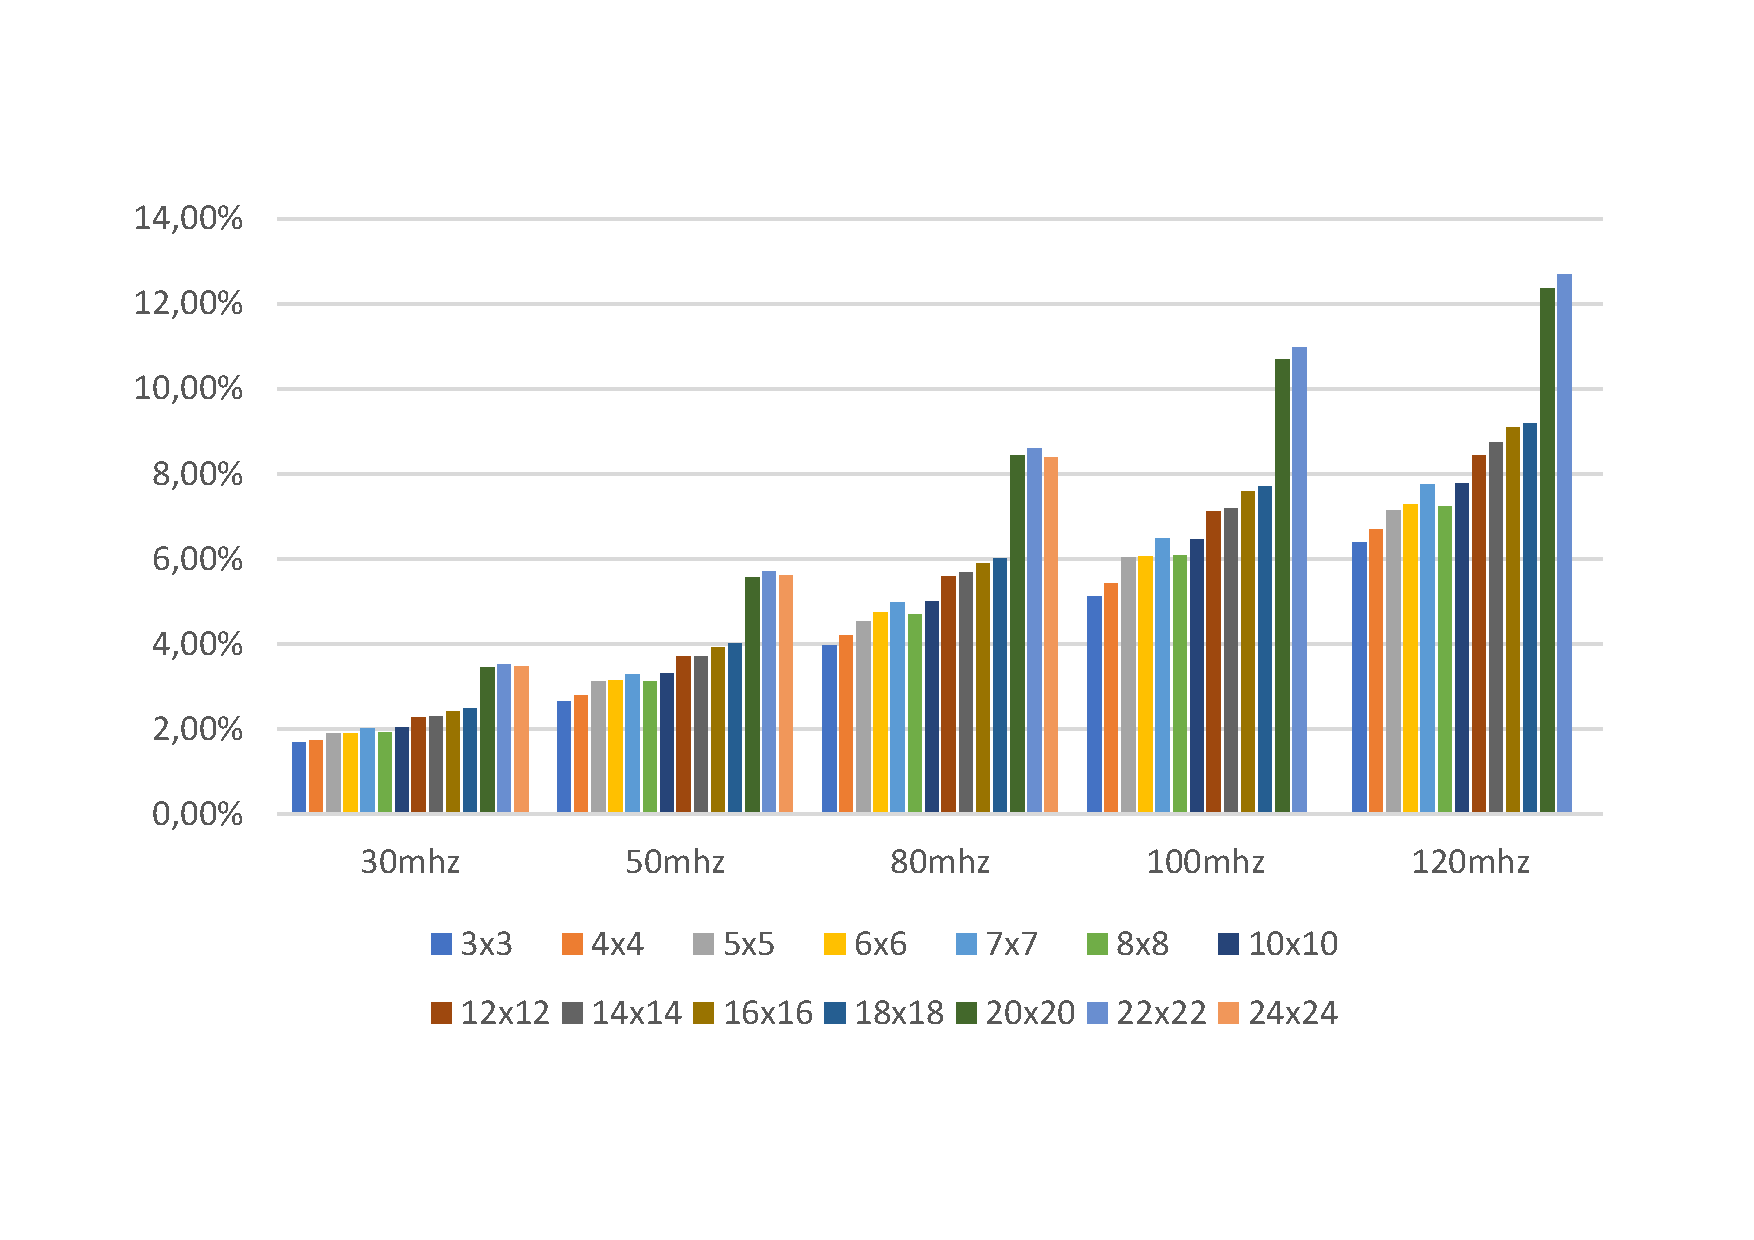
\includegraphics[scale=0.45,angle=0]{./figure/graphs/power_pldyn_int8_freq.pdf}
\caption{Post Implementation Dynamic Power Consumption per Programmable logic with integer 8 PEs}
\label{fig:dynpowint8}
\end{figure}\\\\
The previous Figures represent the behaviour of the power consumption with different Matrix Multiplicatio Unit and for different clock frequency. It is expressed as percentage with reference to the total power consumption of the SoC ( processing system and programmable logic). In fact it can be seen that the power consumption of the processing system and the static power consumption have a less impact on the total power consumption with an increase of the Matrix Multiplication Unit and the frequency. On the other hand, the dynamic power consumption \ref{fig:dynpowint8}, as expected, grows with a growing Matrix Multiplication Unit and the design frequency.\\
In the following Figures, the dynamic power consumption for each entities (in percentage, wrt the dynamic power in Figure \ref{fig:dynpowint8}) in the FPGA is analyzed for different clock frequencies.\\
\begin{figure}[!htbp]
\centering
\captionsetup{justification=centering}
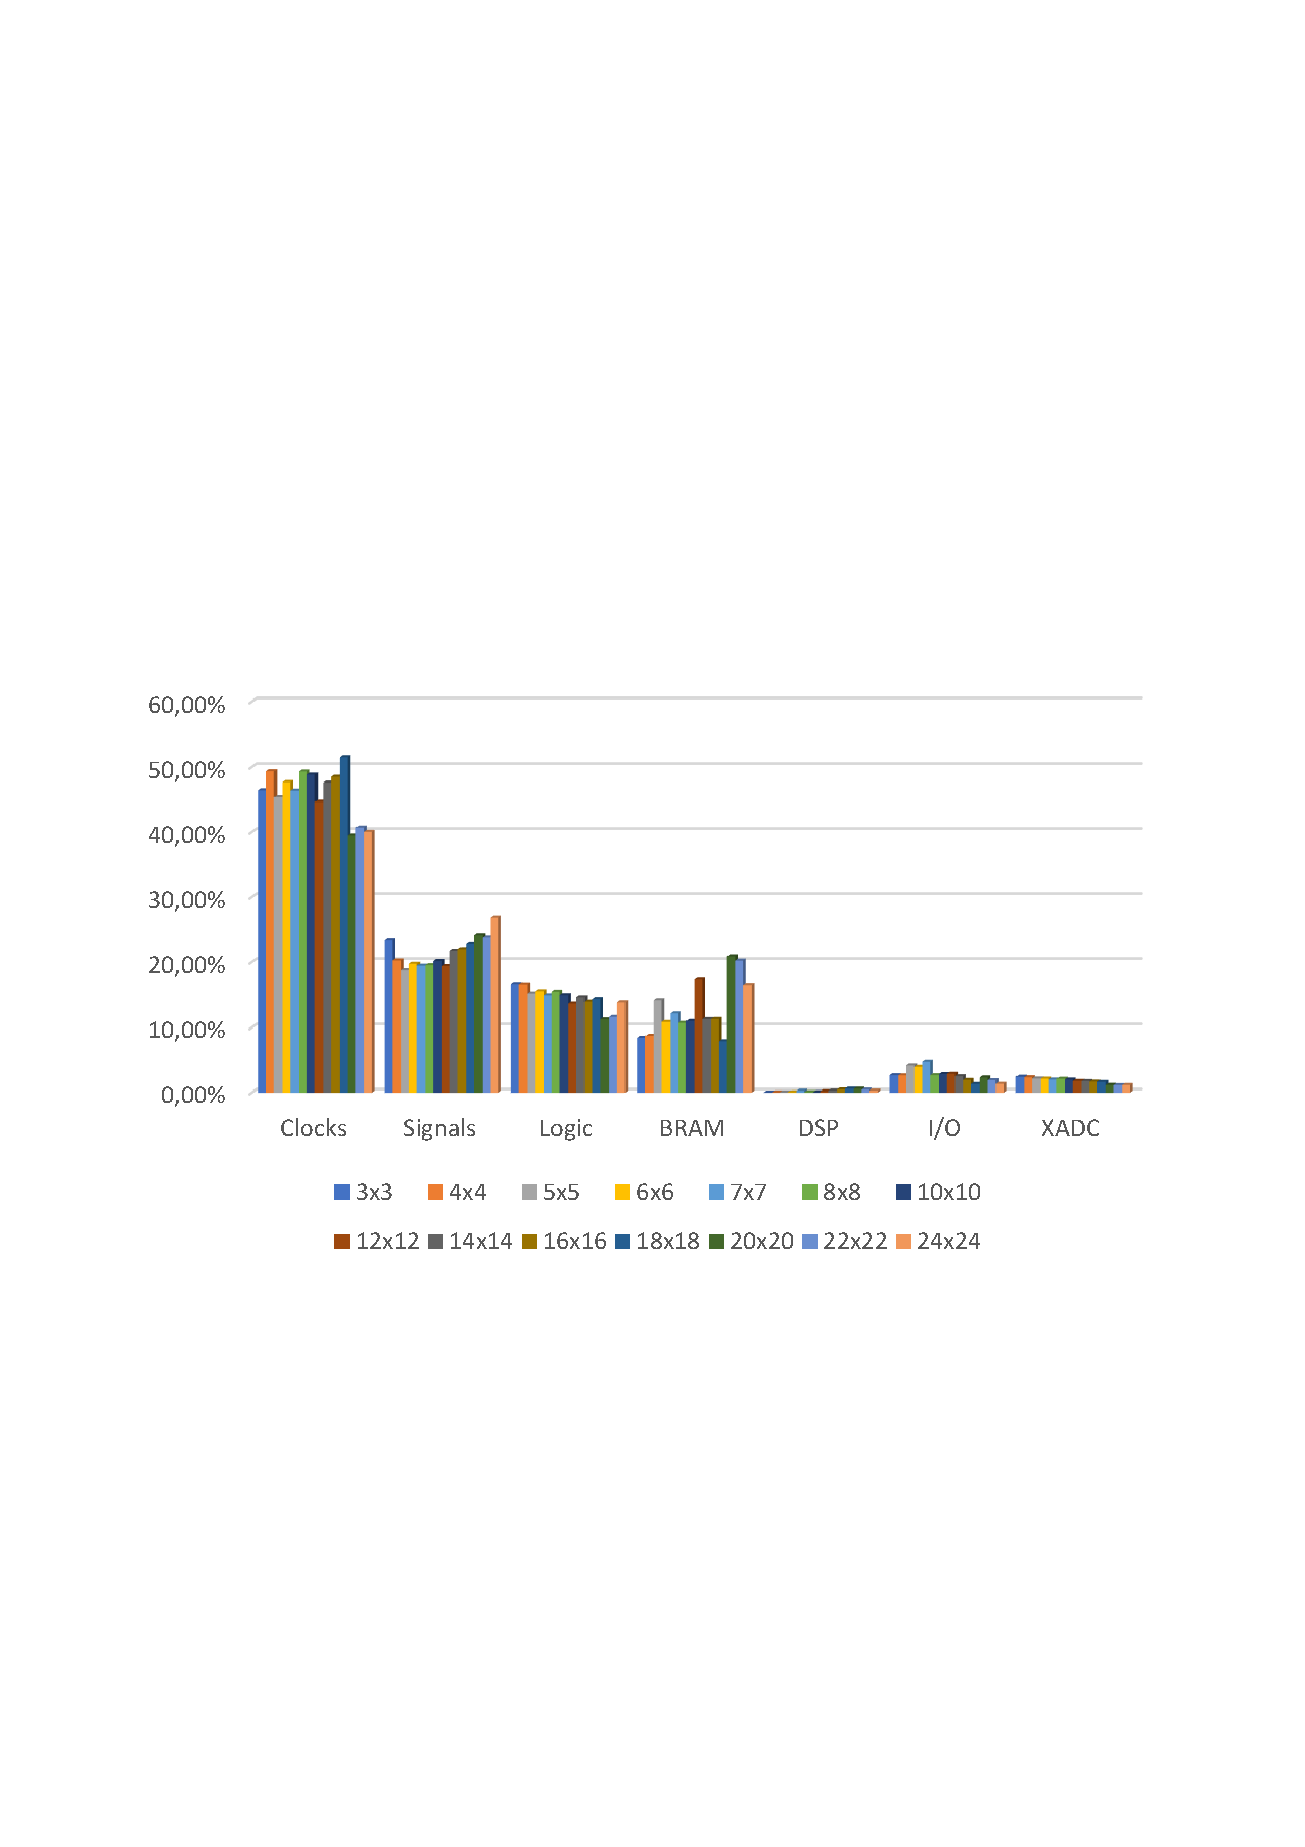
\includegraphics[scale=0.7,angle=0]{./figure/graphs/power_pldyn_div_int8_freq_30mhz.pdf}
\caption{Post Implementation Dynamic Power Consumption per entities in Programmable Logic with a clock frequency of 30 MHz and integer 8 PEs}
\label{fig:dynpowint8ent30}
\end{figure}
\begin{figure}[!htbp]
\centering
\captionsetup{justification=centering}
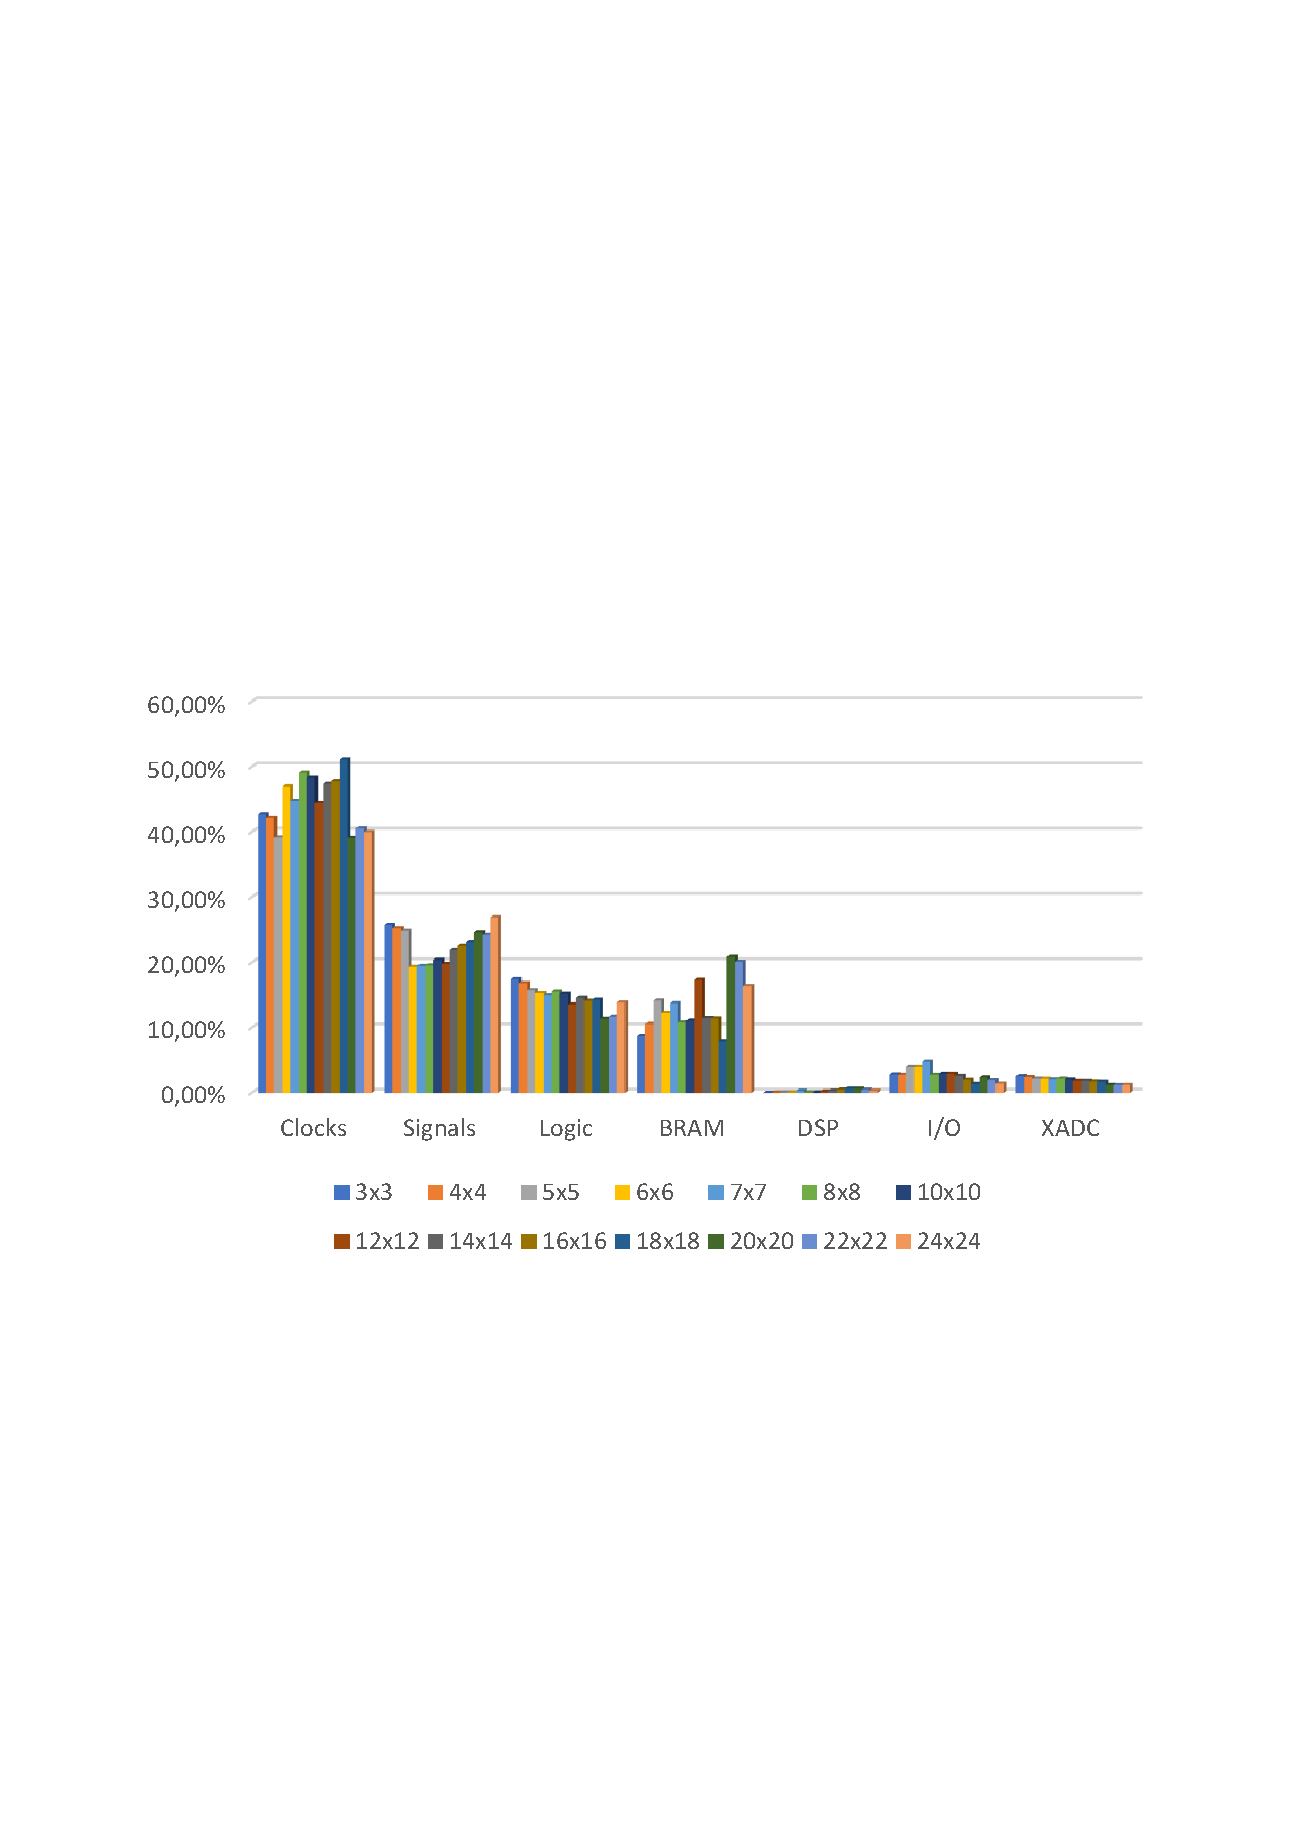
\includegraphics[scale=0.7,angle=0]{./figure/graphs/power_pldyn_div_int8_freq_50mhz.pdf}
\caption{Post Implementation Dynamic Power Consumption per entities in Programmable Logic with a clock frequency of 50 MHz and integer 8 PEs}
\label{fig:dynpowint8ent50}
\end{figure}
\begin{figure}[!htbp]
\centering
\captionsetup{justification=centering}
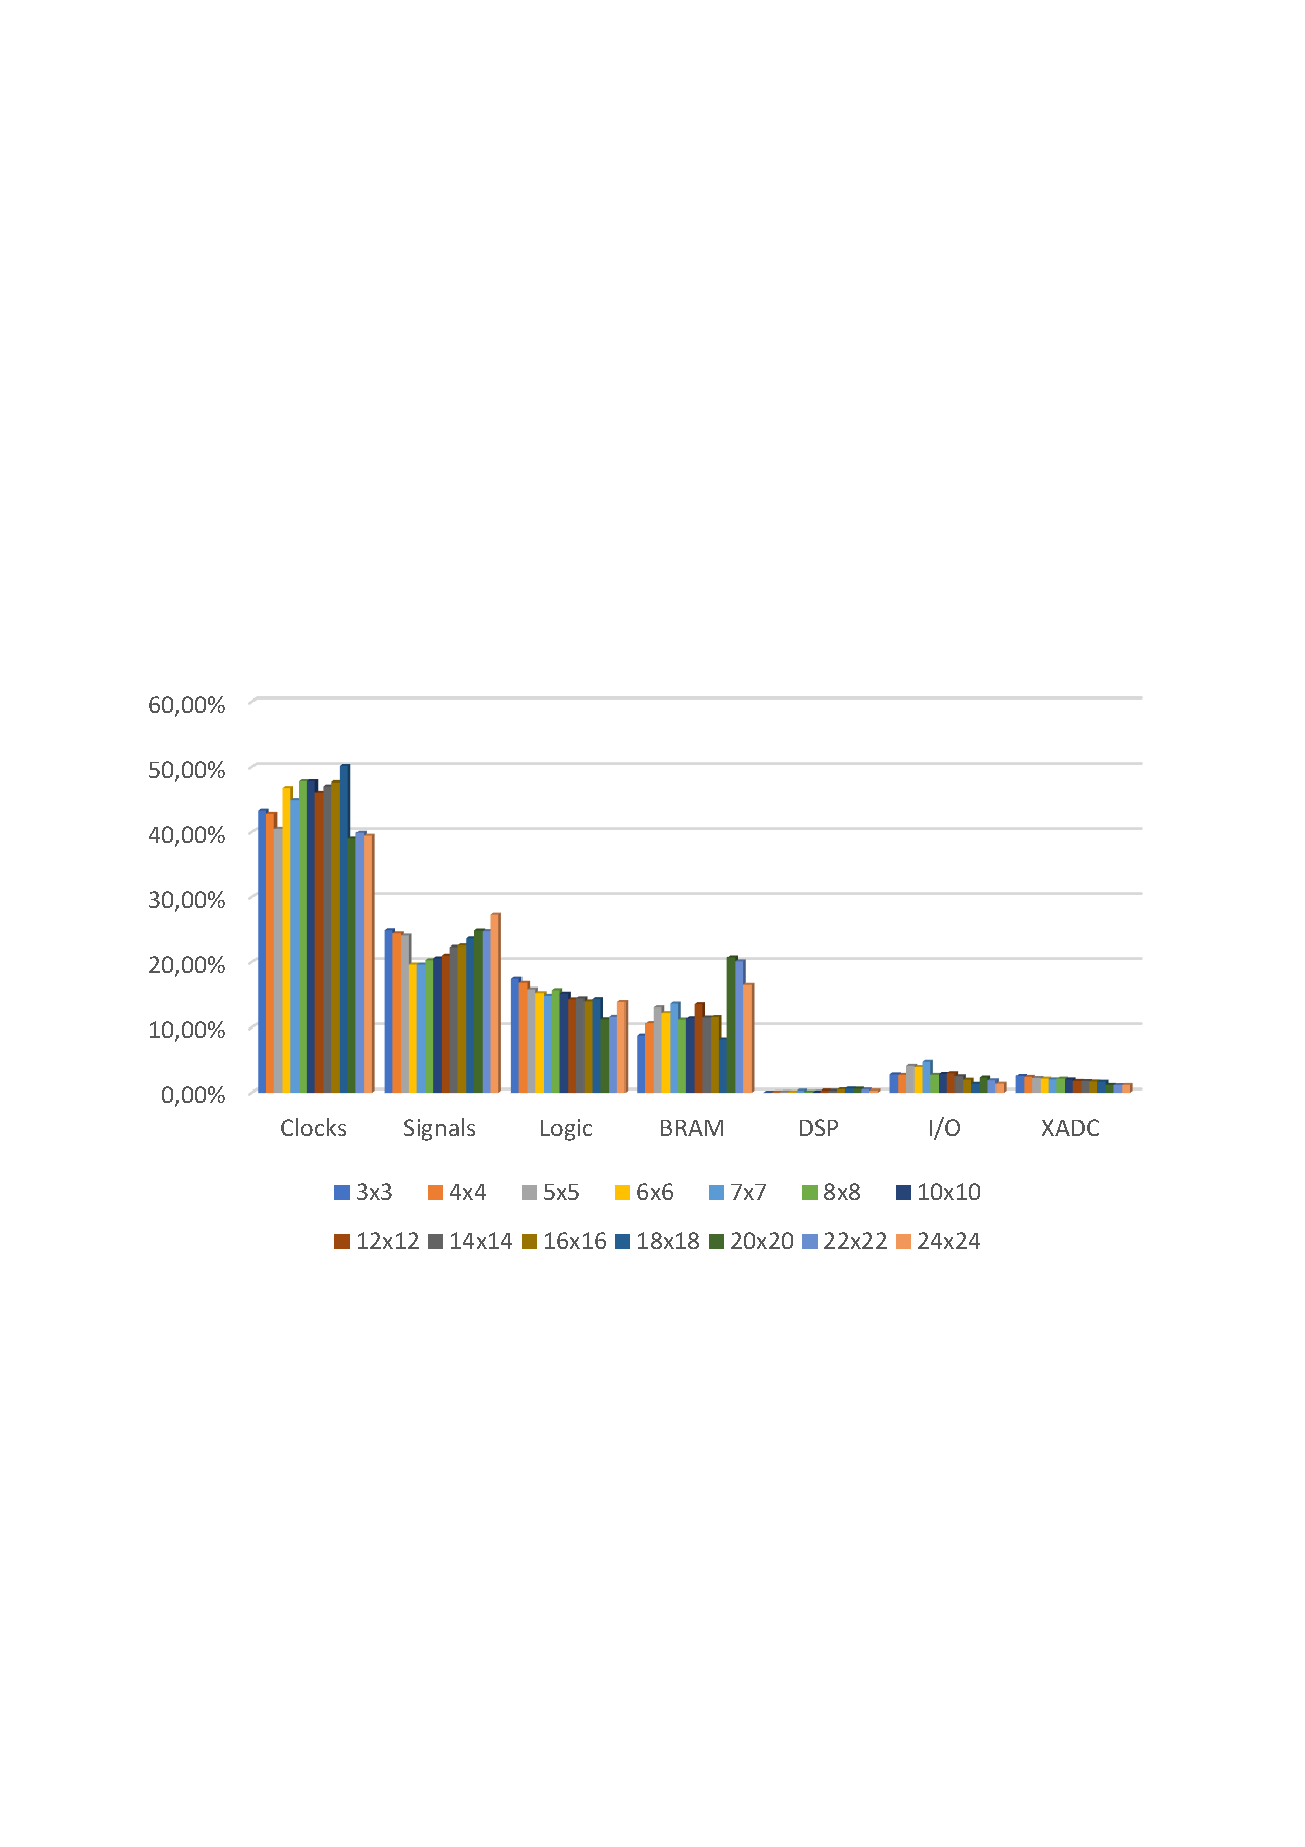
\includegraphics[scale=0.7,angle=0]{./figure/graphs/power_pldyn_div_int8_freq_80mhz.pdf}
\caption{Post Implementation Dynamic Power Consumption per entities in Programmable Logic with a clock frequency of 80 MHz and integer 8 PEs}
\label{fig:dynpowint8ent80}
\end{figure}
\begin{figure}[!htbp]
\centering
\captionsetup{justification=centering}
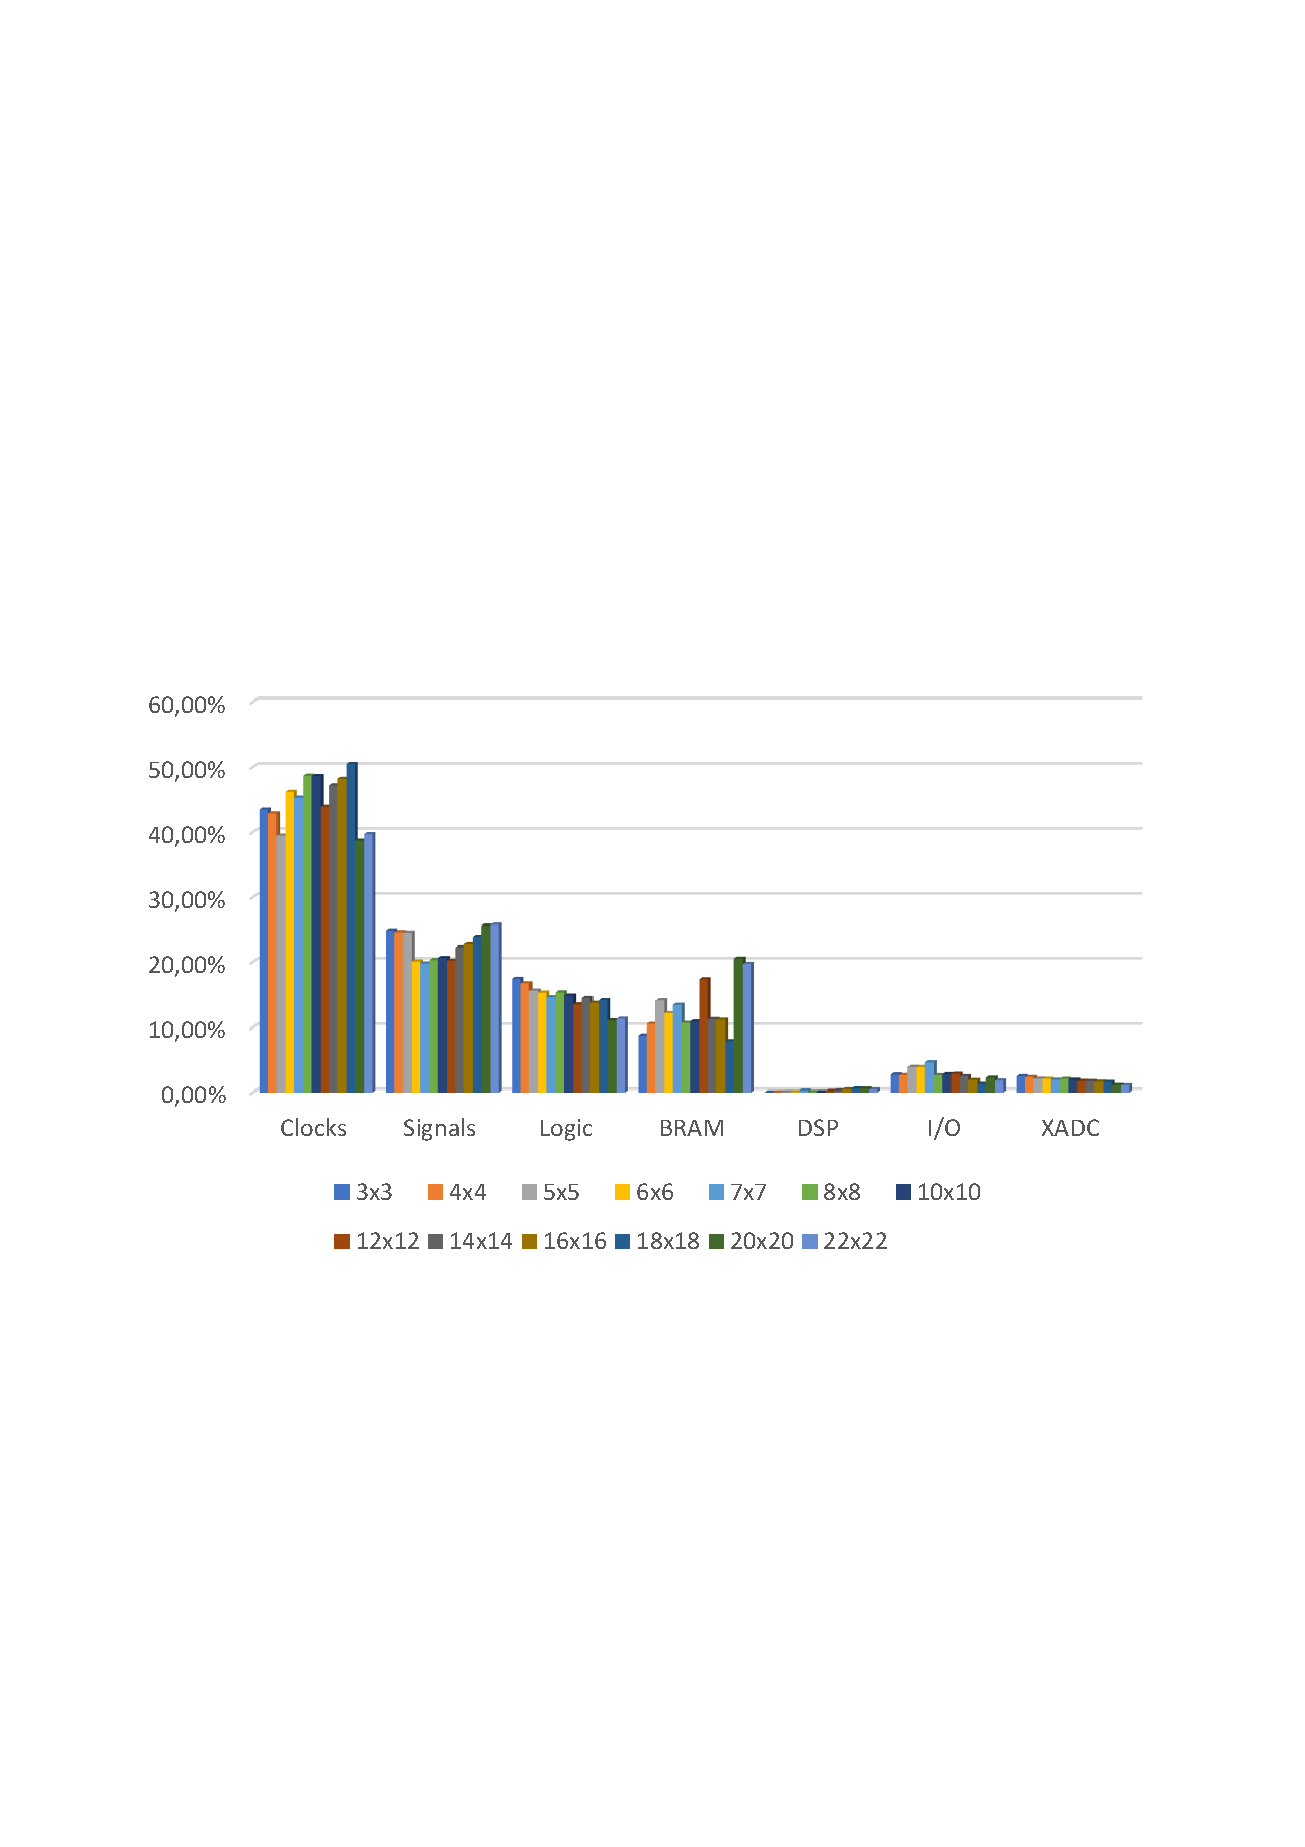
\includegraphics[scale=0.7,angle=0]{./figure/graphs/power_pldyn_div_int8_freq_100mhz.pdf}
\caption{Post Implementation Dynamic Power Consumption per entities in Programmable Logic with a clock frequency of 100 MHz and integer 8 PEs}
\label{fig:dynpowint8ent100}
\end{figure}
\begin{figure}[!htbp]
\centering
\captionsetup{justification=centering}
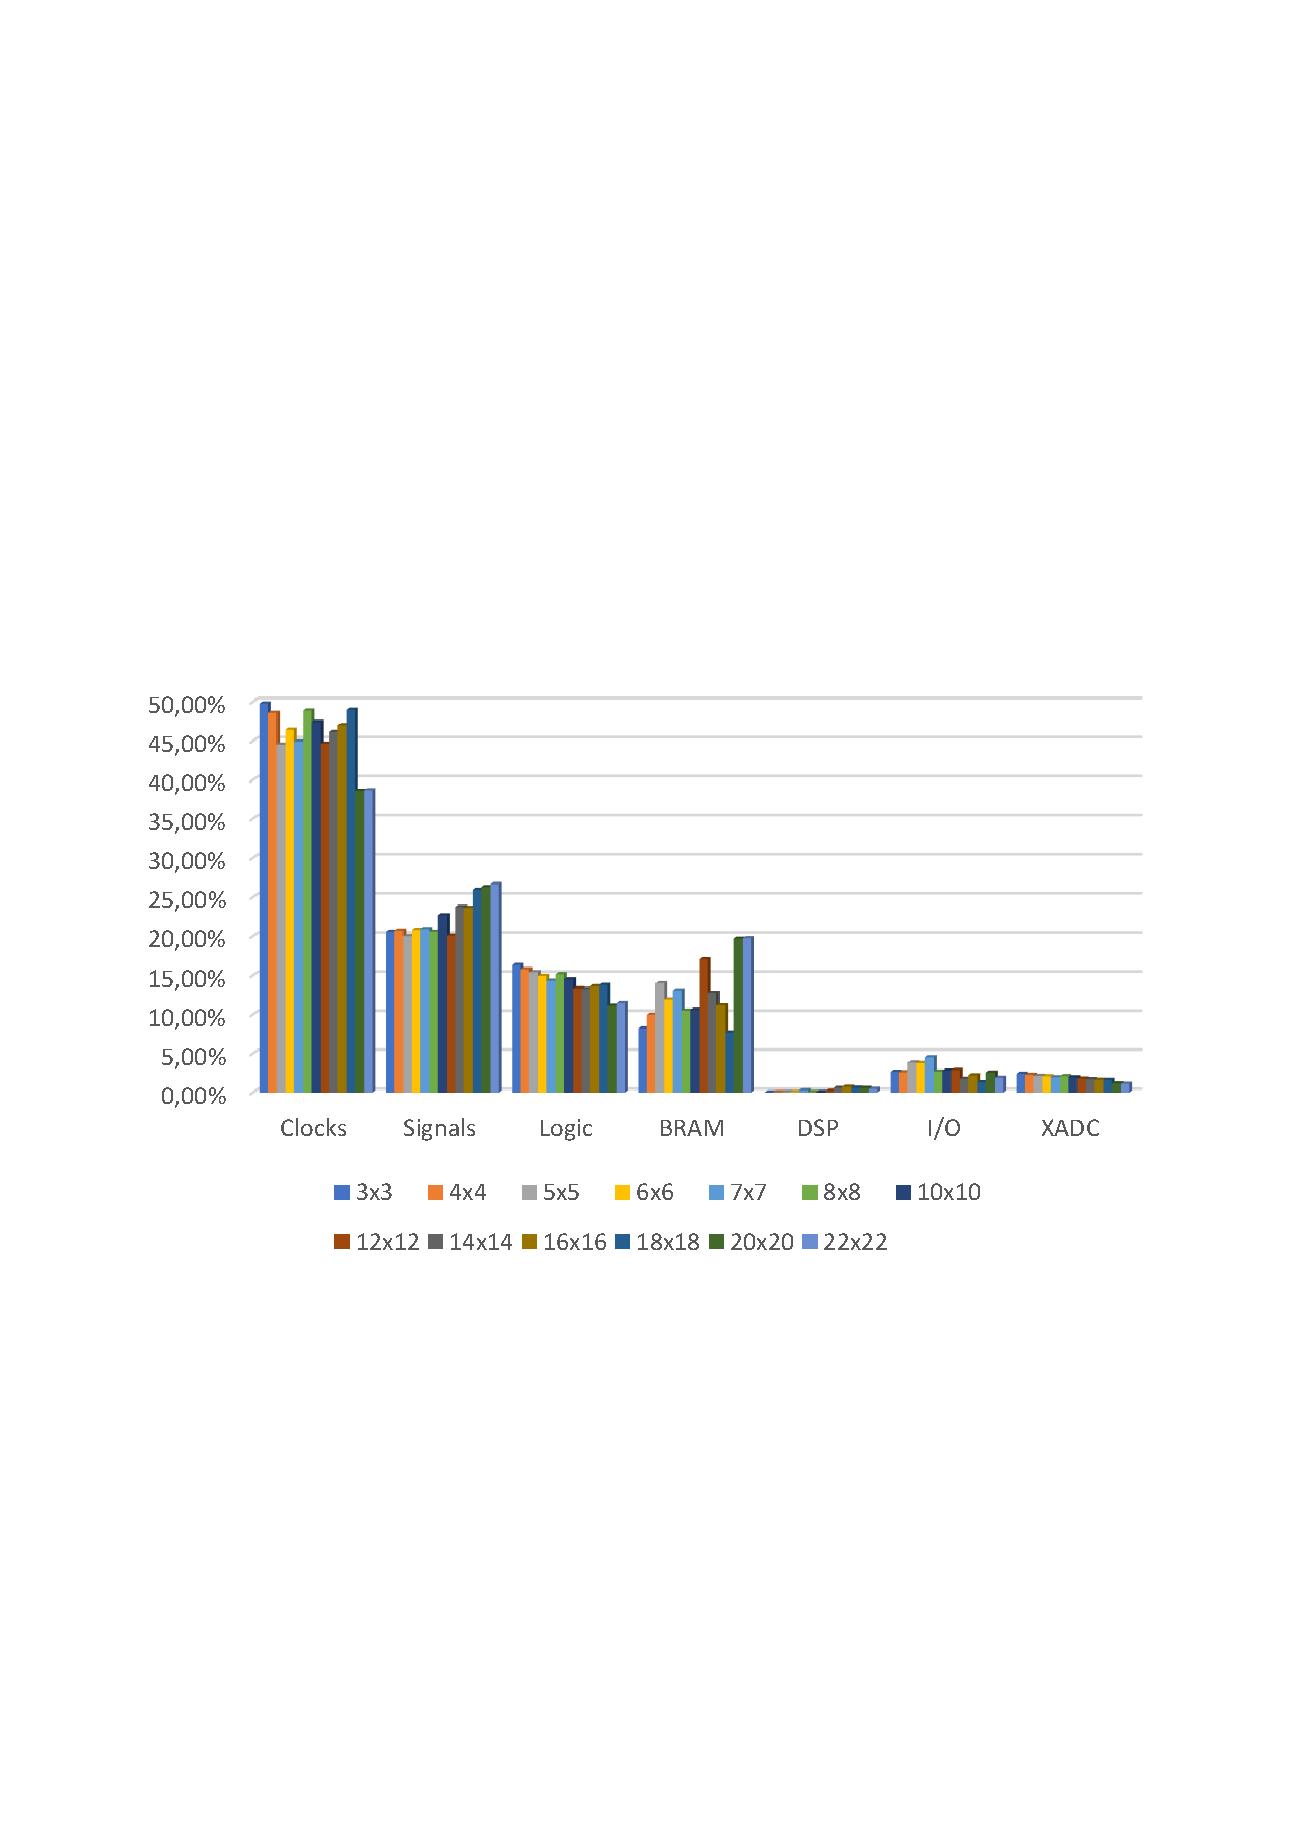
\includegraphics[scale=0.7,angle=0]{./figure/graphs/power_pldyn_div_int8_freq_120mhz.pdf}
\caption{Post Implementation Dynamic Power Consumption per entities in Programmable Logic with a clock frequency of 120 MHz and integer 8 PEs}
\label{fig:dynpowint8ent120}
\end{figure}\\\\
As it is very well known, the clock distribution is one of the main source of power consumption, and it is confirmed from all the previos Figures. Also the interconnections, called \textit{signals} in the figures, are power hungry (a bigger MXU leads to many, and longer, interconnections between PEs). In fact the clock distribution networks and the interconnections are the predominant entities of the dynamic power consumption of the programmable logic.
The logic entity is containing all the power consumed by the FFs and LUTs, it looks like their power consumption is decreasing but it is only the percentage of the total dynamic power which is decreasing.
It is worth to mention that the PEs (at least the majority of them) are implemented using the DSP entities. However, the power consumed by those entities is almost negligible,  the DSPs are low power entities in the FGPA according to its datasheet \cite{paper:42}.\\
Regarding the BRAM, I/O and XADC, with an increase or a decrease of the other entities impact they have a slightly modification of their impact on the power consumption.\\
\item Integer 16:\\
In the follwing Figures, the same considerations for the Integer 8 are still valid since the PEs are always implemented on the same DSP entity but without the higher 8 bits of the input values gated to zeros.
\begin{figure}[!htbp]
\centering
\captionsetup{justification=centering}
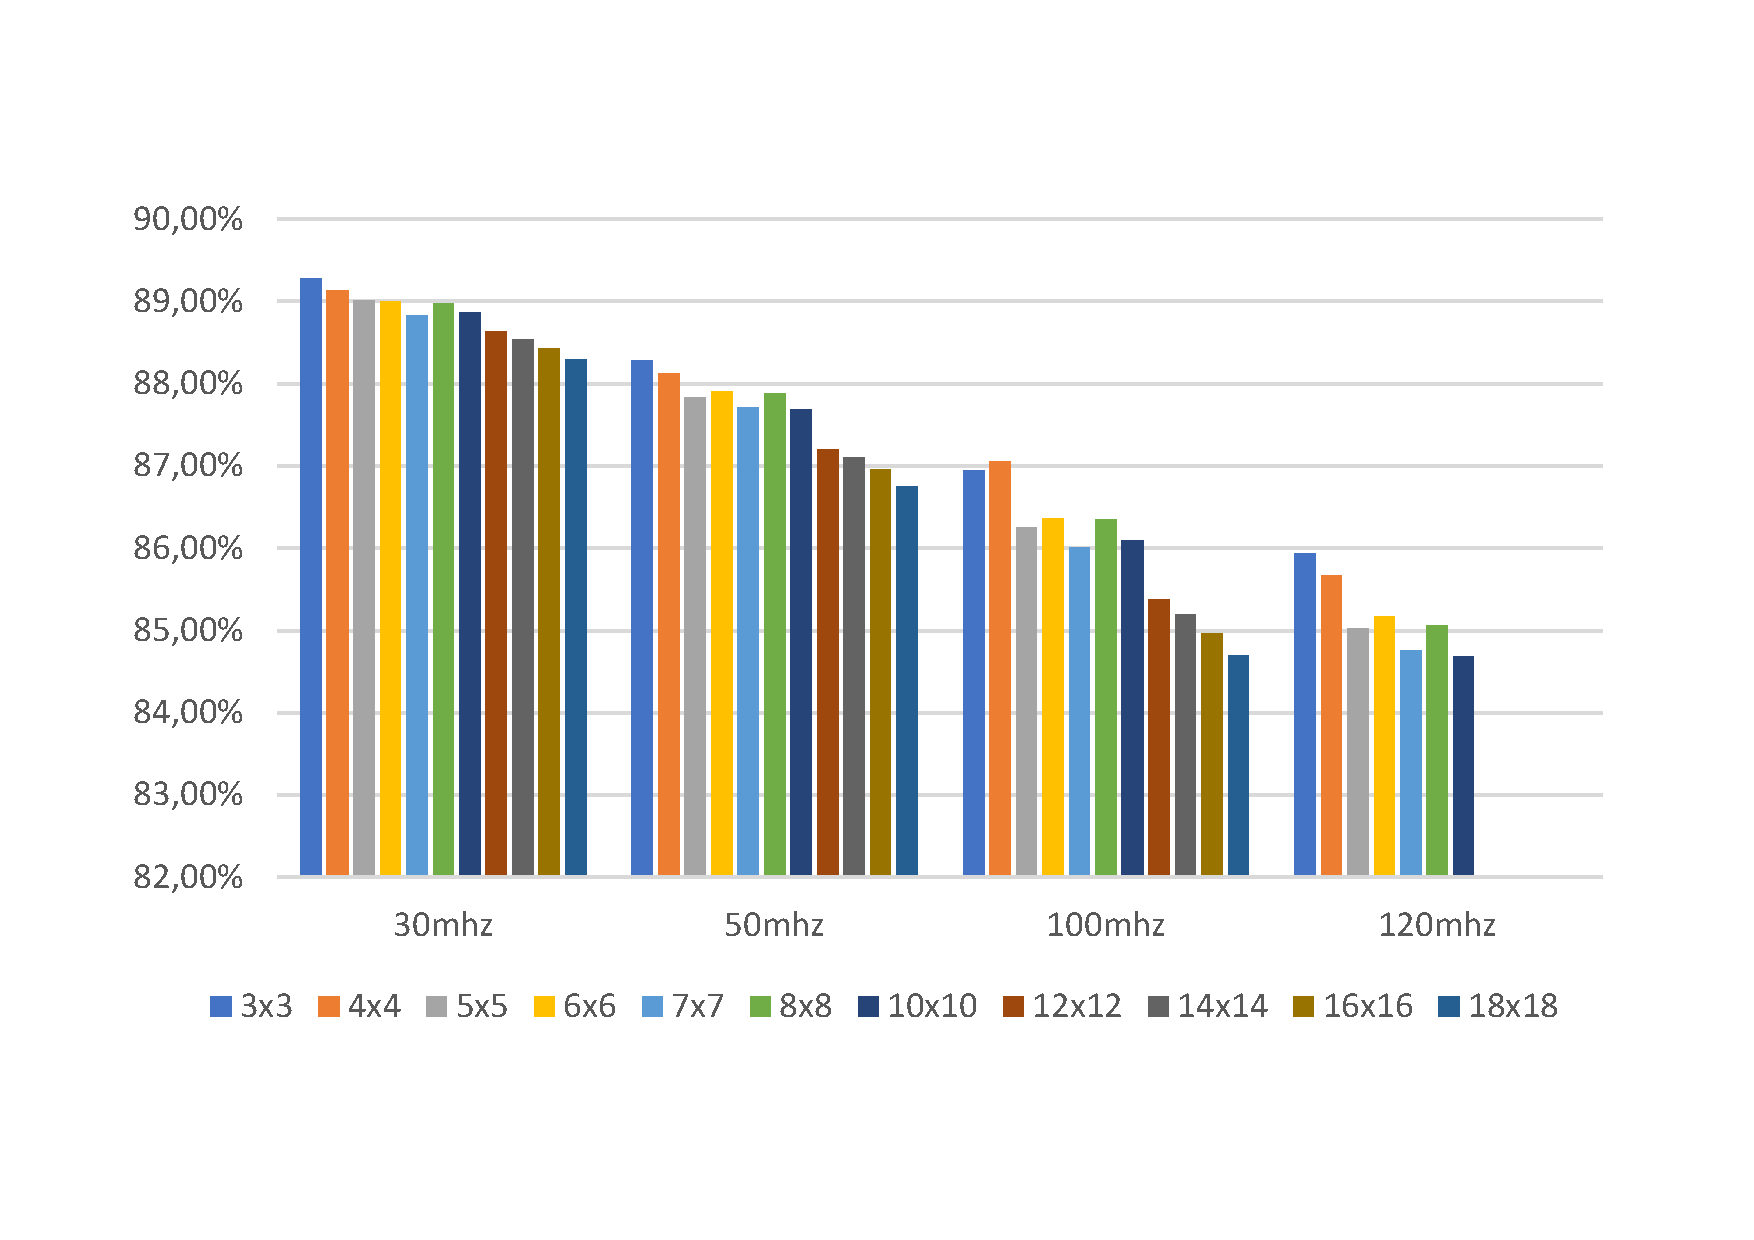
\includegraphics[scale=0.5,angle=0]{./figure/graphs/power_ps_int16_freq.pdf}
\caption{Post Implementation Power Consumption of Processing System for integer 16 PEs}
\label{fig:powint16}
\end{figure}
\begin{figure}[!htbp]
\centering
\captionsetup{justification=centering}
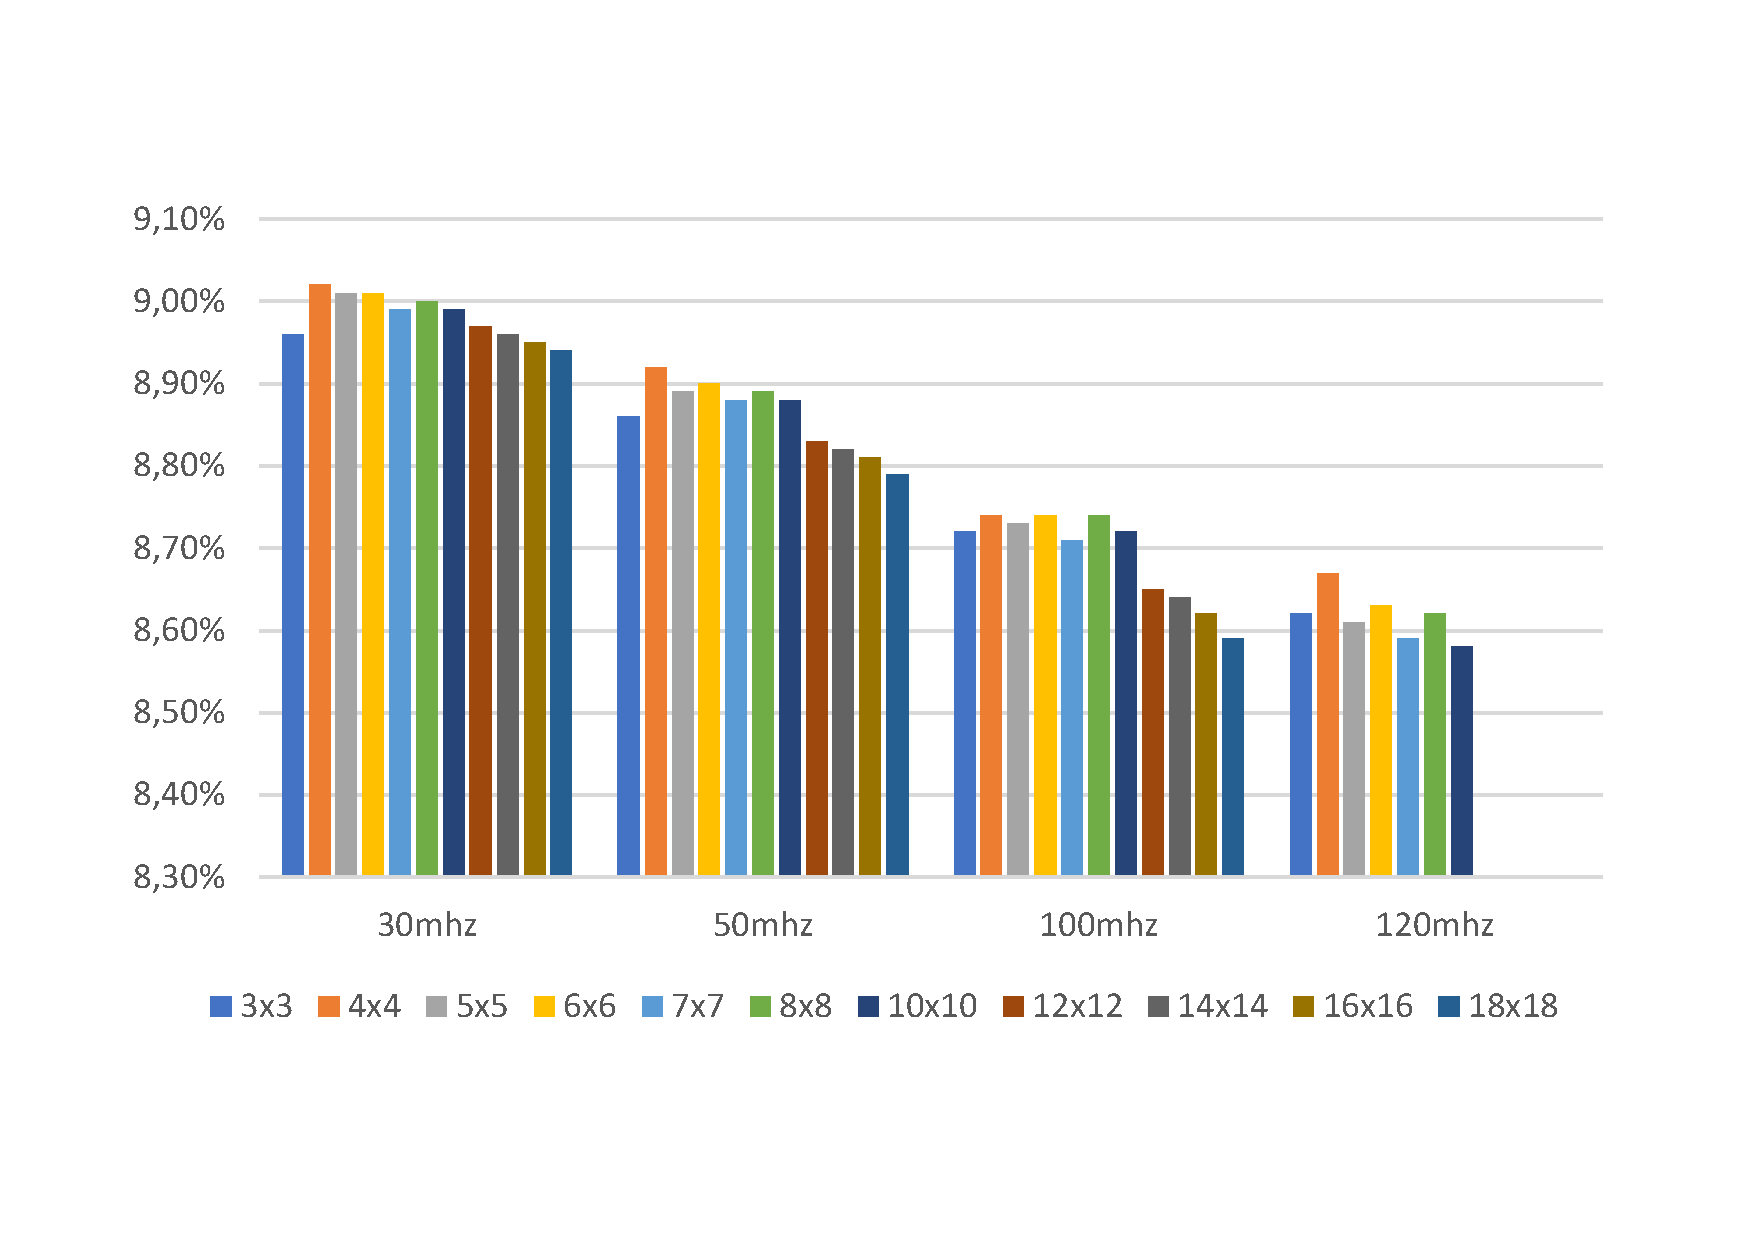
\includegraphics[scale=0.5,angle=0]{./figure/graphs/power_plstatic_int16_freq.pdf}
\caption{Post Implementation Static Power Consumption Programmable logic for integer 16 PEs }
\label{fig:staticpowint16}
\end{figure}
\begin{figure}[!htbp]
\centering
\captionsetup{justification=centering}
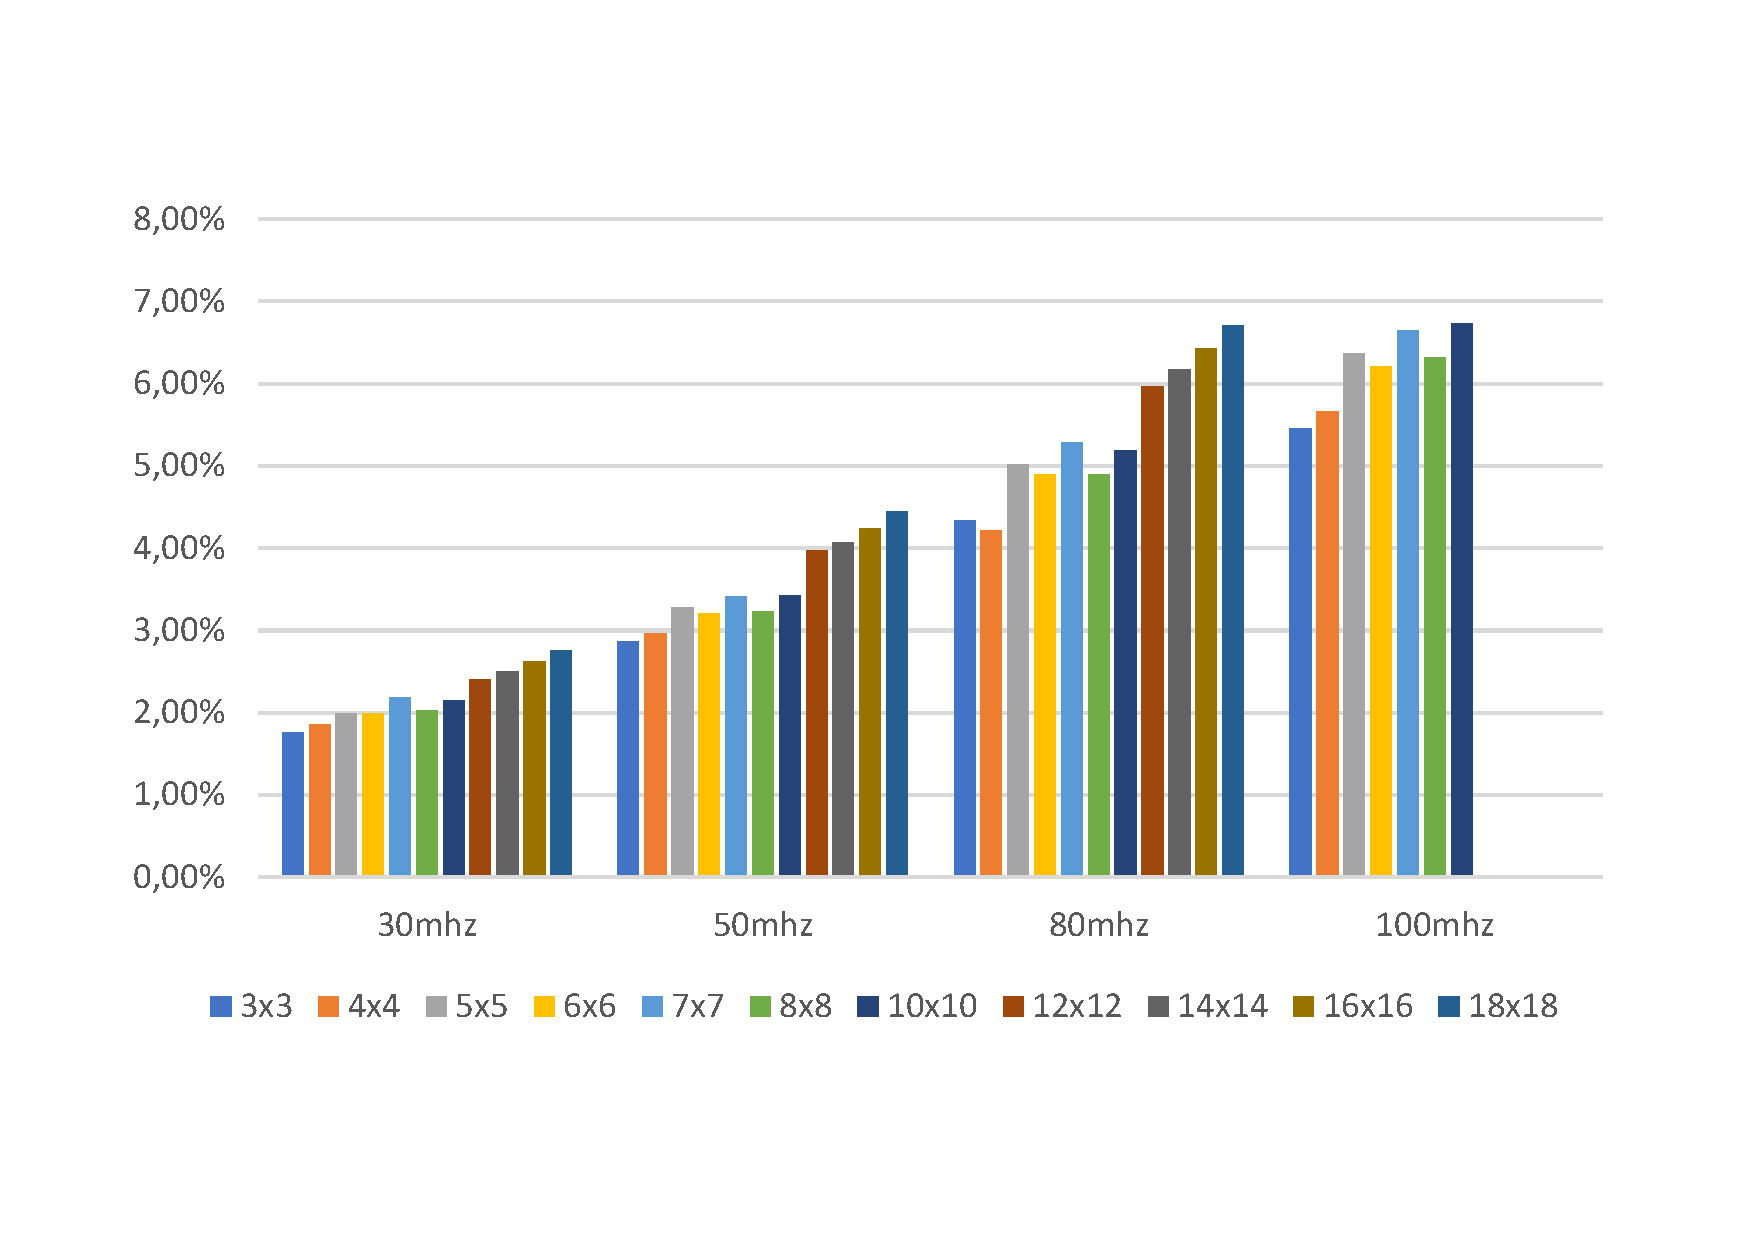
\includegraphics[scale=0.5,angle=0]{./figure/graphs/power_pldyn_int16_freq.pdf}
\caption{Post Implementation Dynamic Power Consumption per Programmable logic with integer 16 PEs}
\label{fig:dynpowint16}
\end{figure}
\begin{figure}[!htbp]
\centering
\captionsetup{justification=centering}
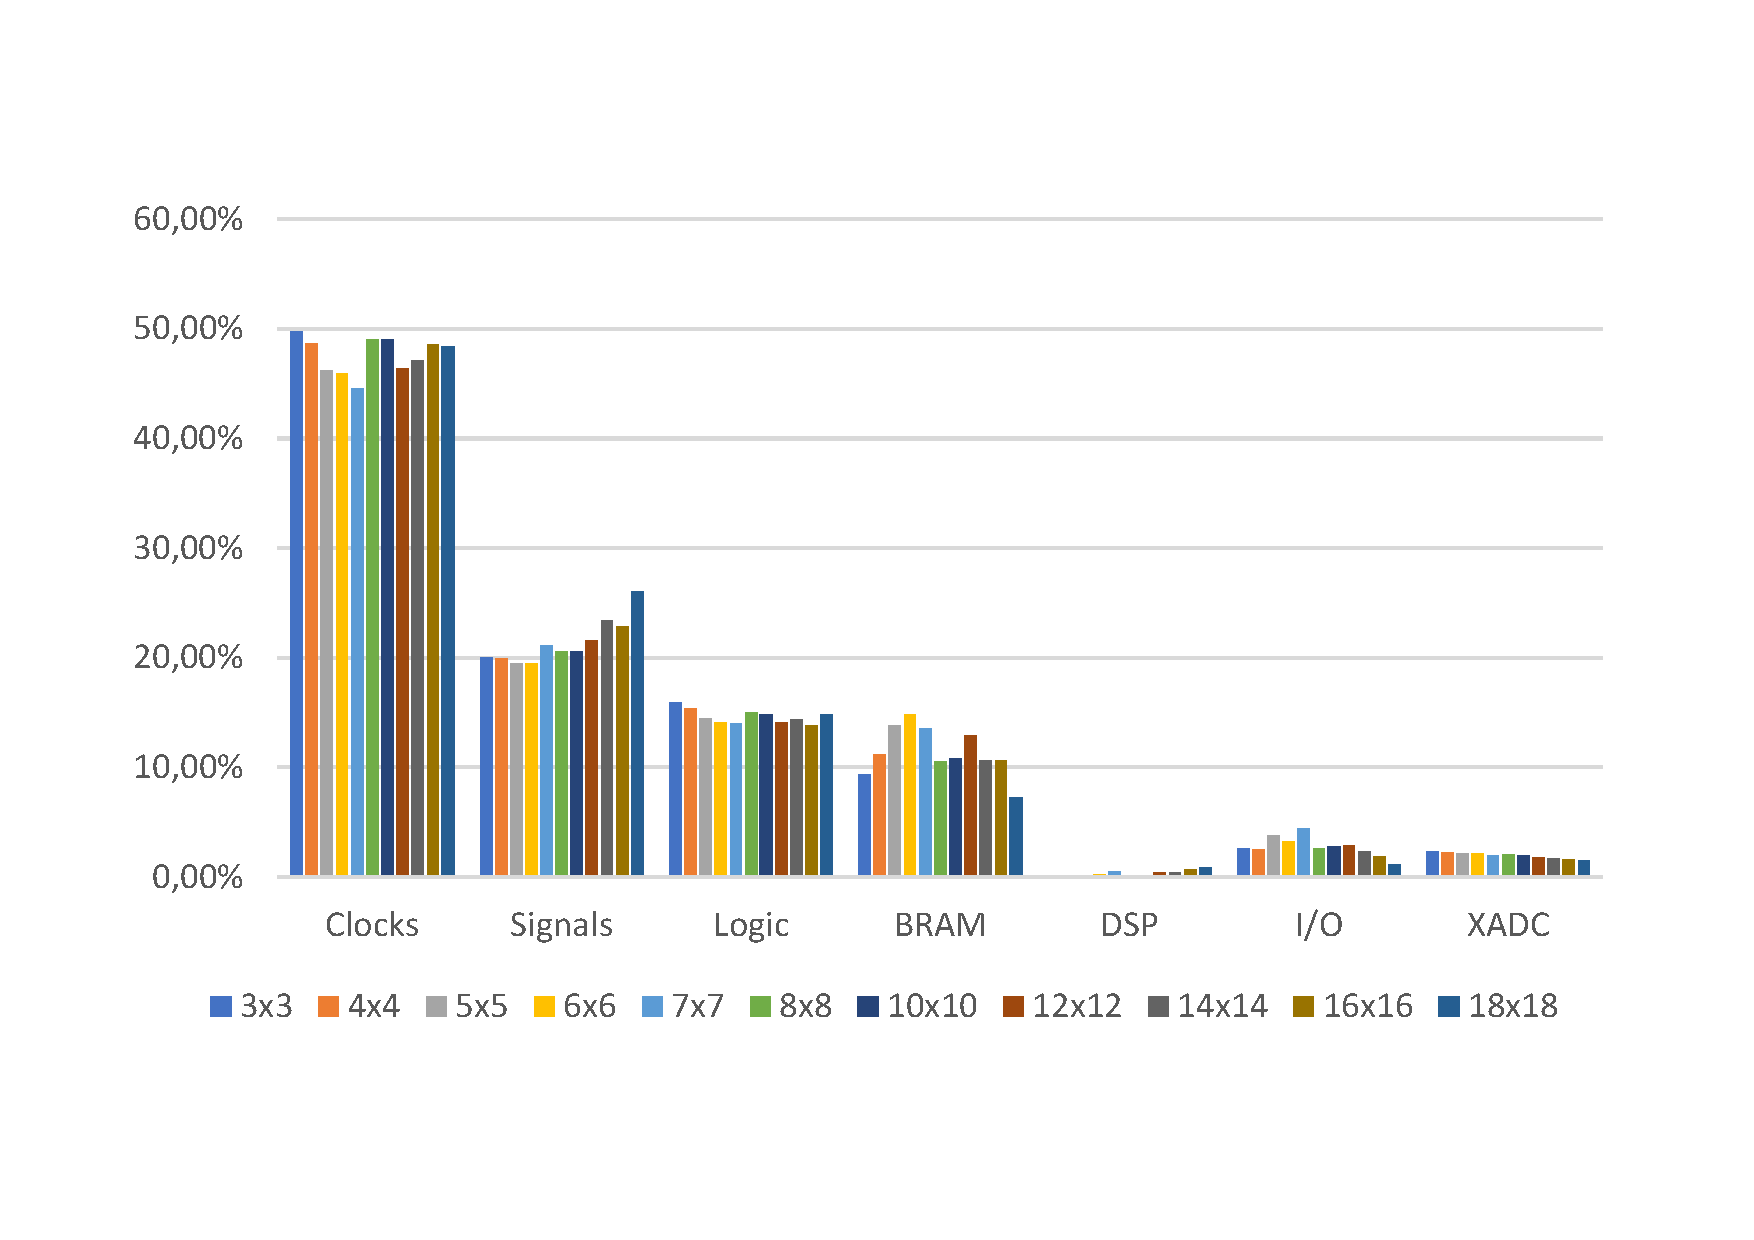
\includegraphics[scale=0.6,angle=0]{./figure/graphs/power_pldyn_div_int16_freq_30mhz.pdf}
\caption{Post Implementation Dynamic Power Consumption per entities in Programmable Logic with a clock frequency of 30 MHz and integer 16 PEs}
\label{fig:dynpowint16ent30}
\end{figure}
\begin{figure}[!htbp]
\centering
\captionsetup{justification=centering}
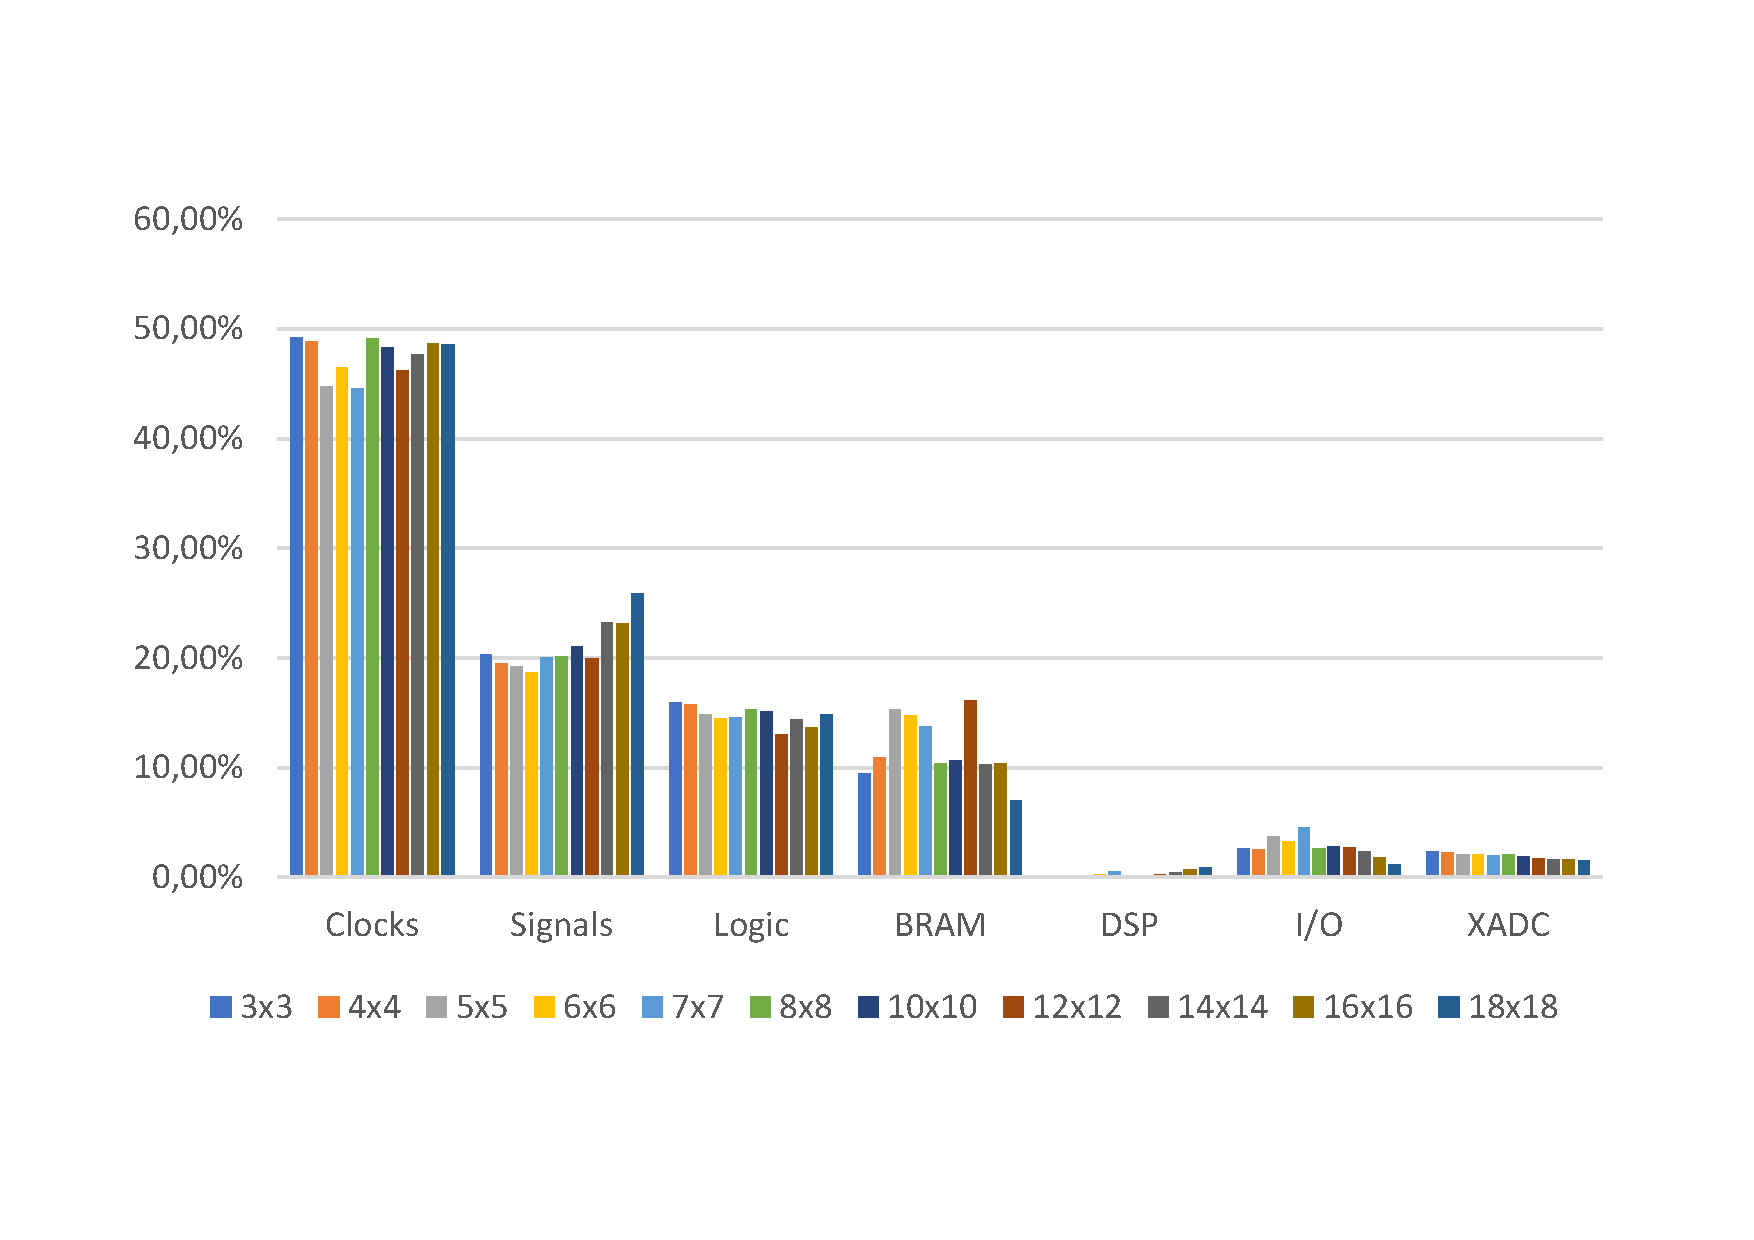
\includegraphics[scale=0.6,angle=0]{./figure/graphs/power_pldyn_div_int16_freq_50mhz.pdf}
\caption{Post Implementation Dynamic Power Consumption per entities in Programmable Logic with a clock frequency of 50 MHz and integer 16 PEs}
\label{fig:dynpowint16ent50}
\end{figure}
\begin{figure}[!htbp]
\centering
\captionsetup{justification=centering}
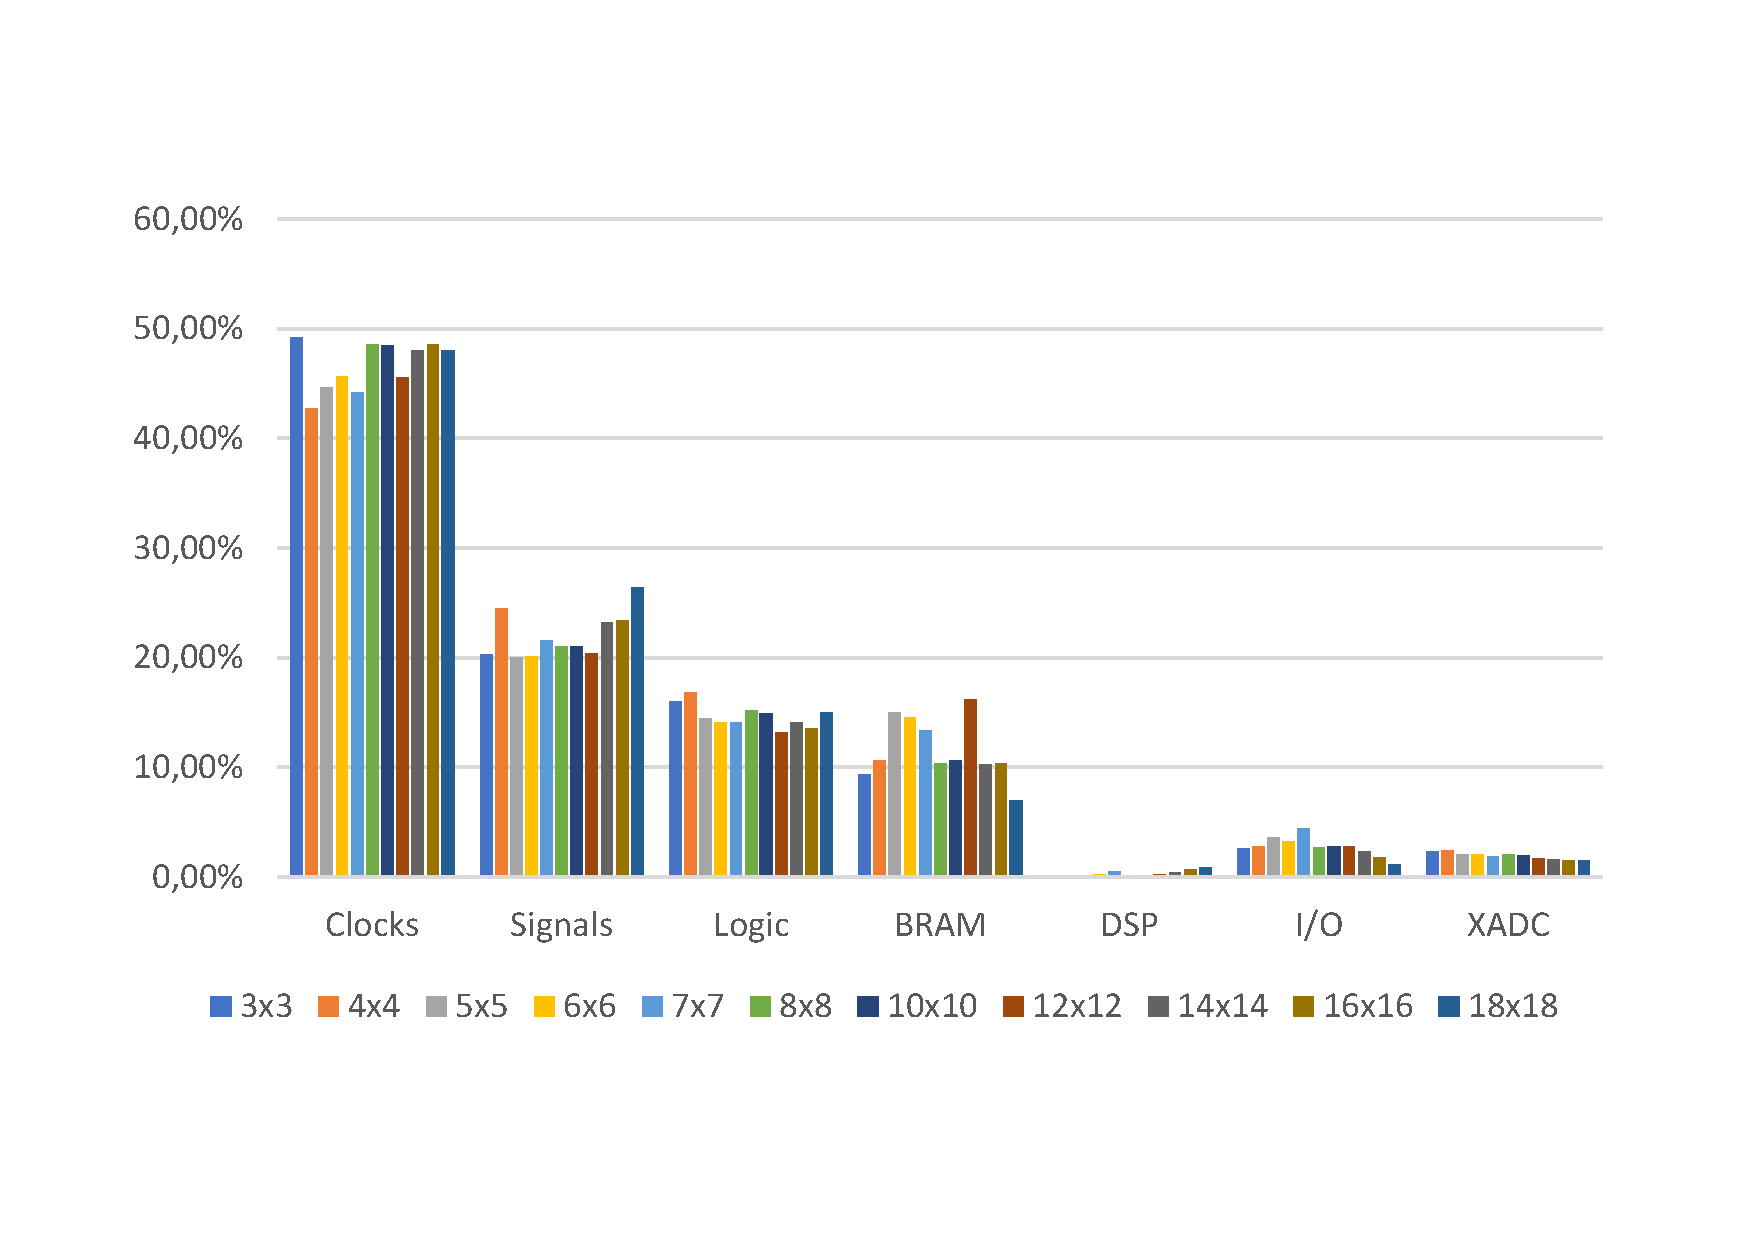
\includegraphics[scale=0.6,angle=0]{./figure/graphs/power_pldyn_div_int16_freq_80mhz.pdf}
\caption{Post Implementation Dynamic Power Consumption per entities in Programmable Logic with a clock frequency of 80 MHz and integer 16 PEs}
\label{fig:dynpowint16ent80}
\end{figure}
\begin{figure}[!htbp]
\centering
\captionsetup{justification=centering}
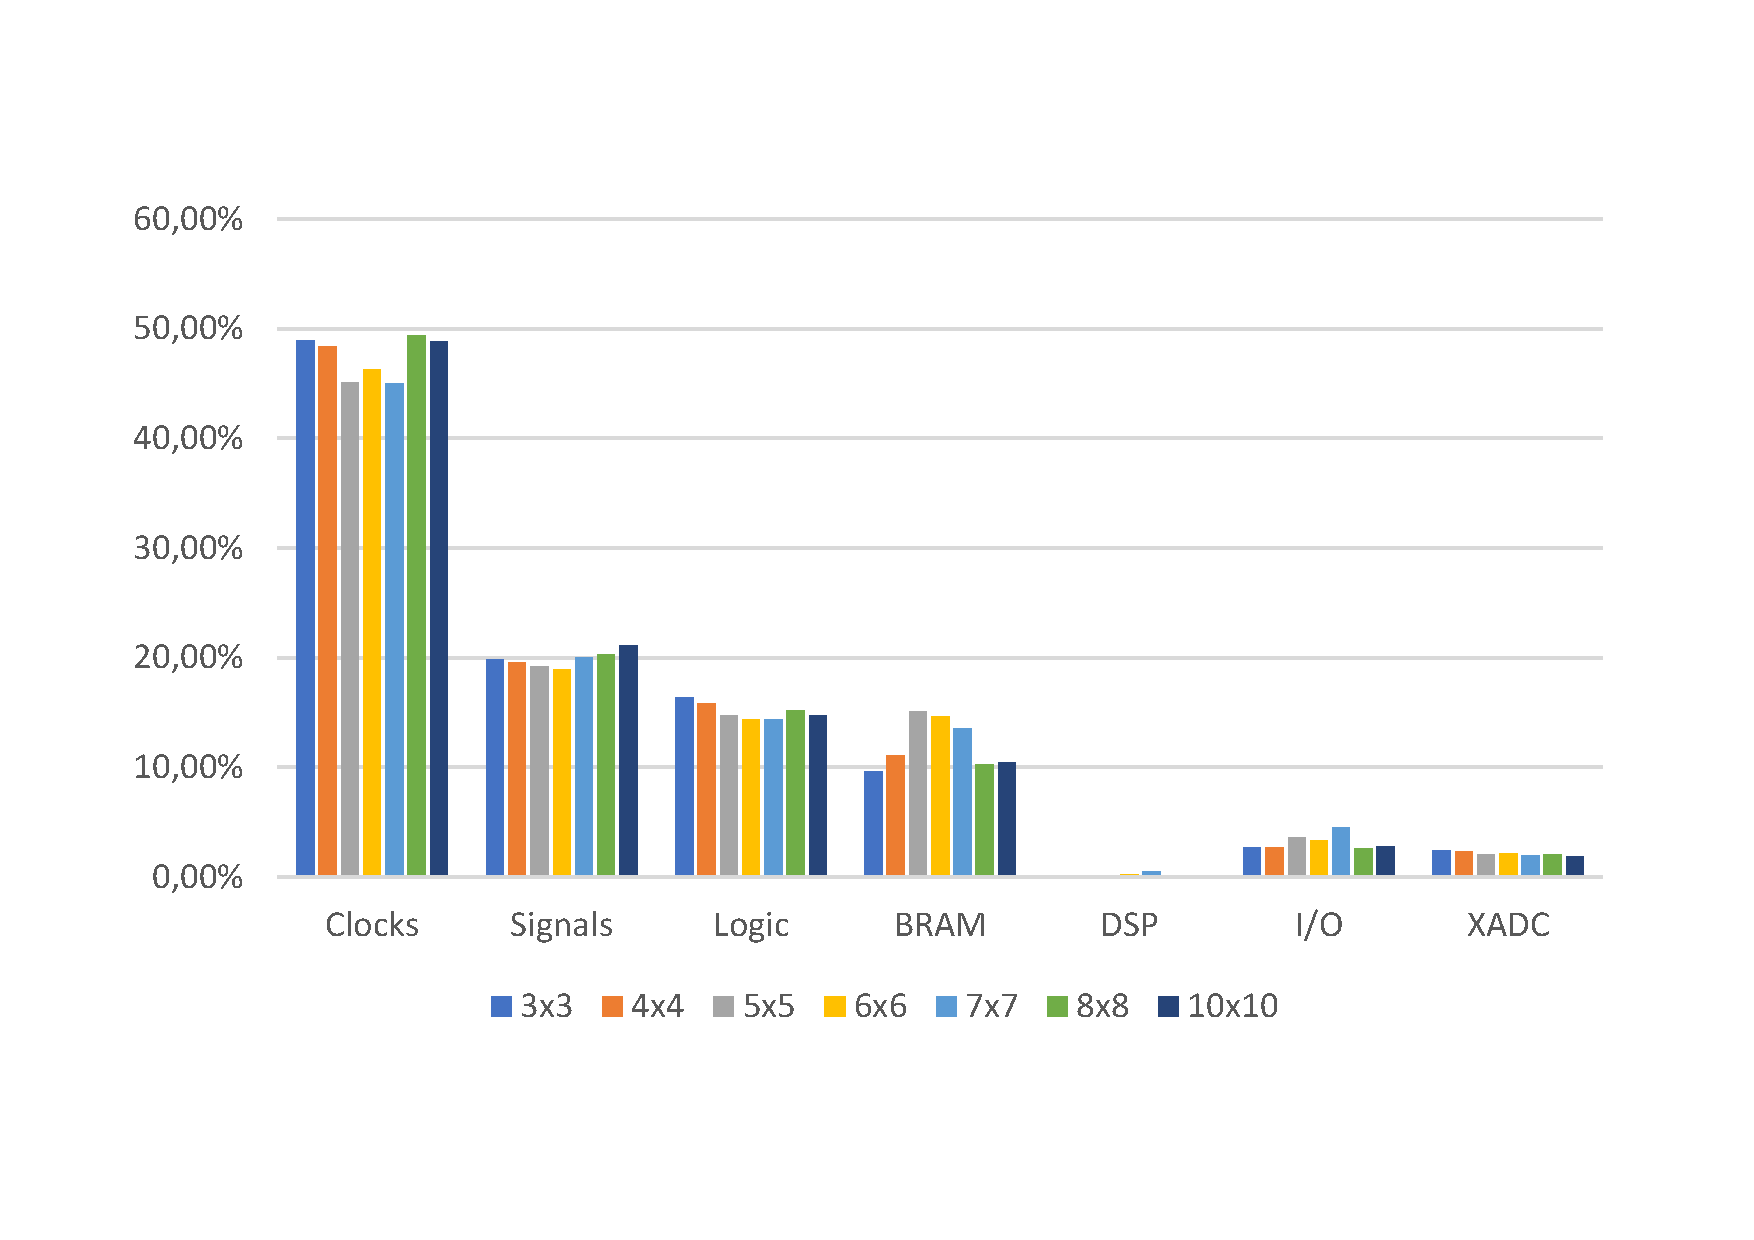
\includegraphics[scale=0.6,angle=0]{./figure/graphs/power_pldyn_div_int16_freq_100mhz.pdf}
\caption{Post Implementation Dynamic Power Consumption per entities in Programmable Logic with a clock frequency of 100 MHz and integer 16 PEs}
\label{fig:dynpowint16ent100}
\end{figure}
\newpage
\item Integer 32:\\
From now on, the MXU sizes and the frequencies will show a reduction in their values, this is manly because big designs (with almost full FPGA's utilization) are not able to meet anymore the timing requirements.
\begin{figure}[!htbp]
\centering
\captionsetup{justification=centering}
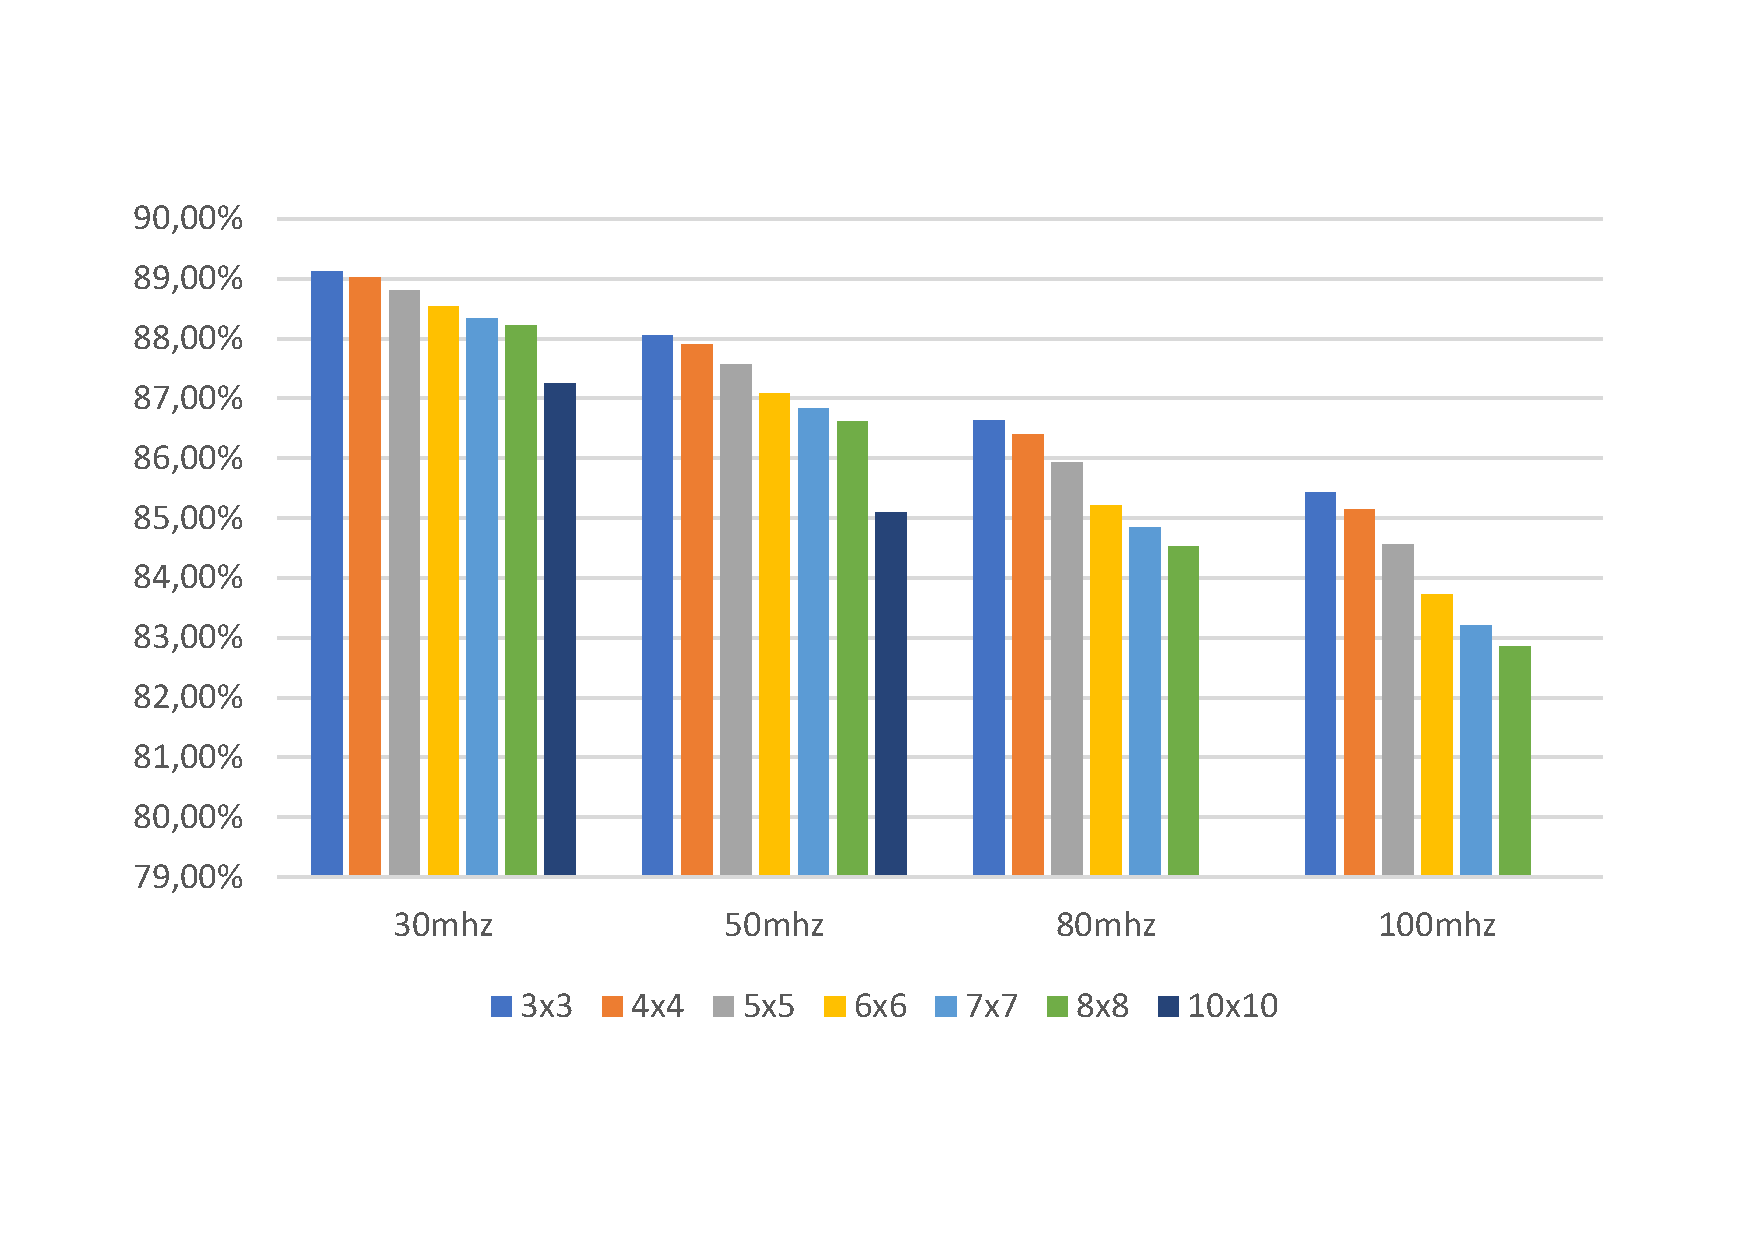
\includegraphics[scale=0.5,angle=0]{./figure/graphs/power_ps_int32_freq.pdf}
\caption{Post Implementation Power Consumption of Processing System for integer 32 PEs}
\label{fig:powint32}
\end{figure}
\begin{figure}[!htbp]
\centering
\captionsetup{justification=centering}
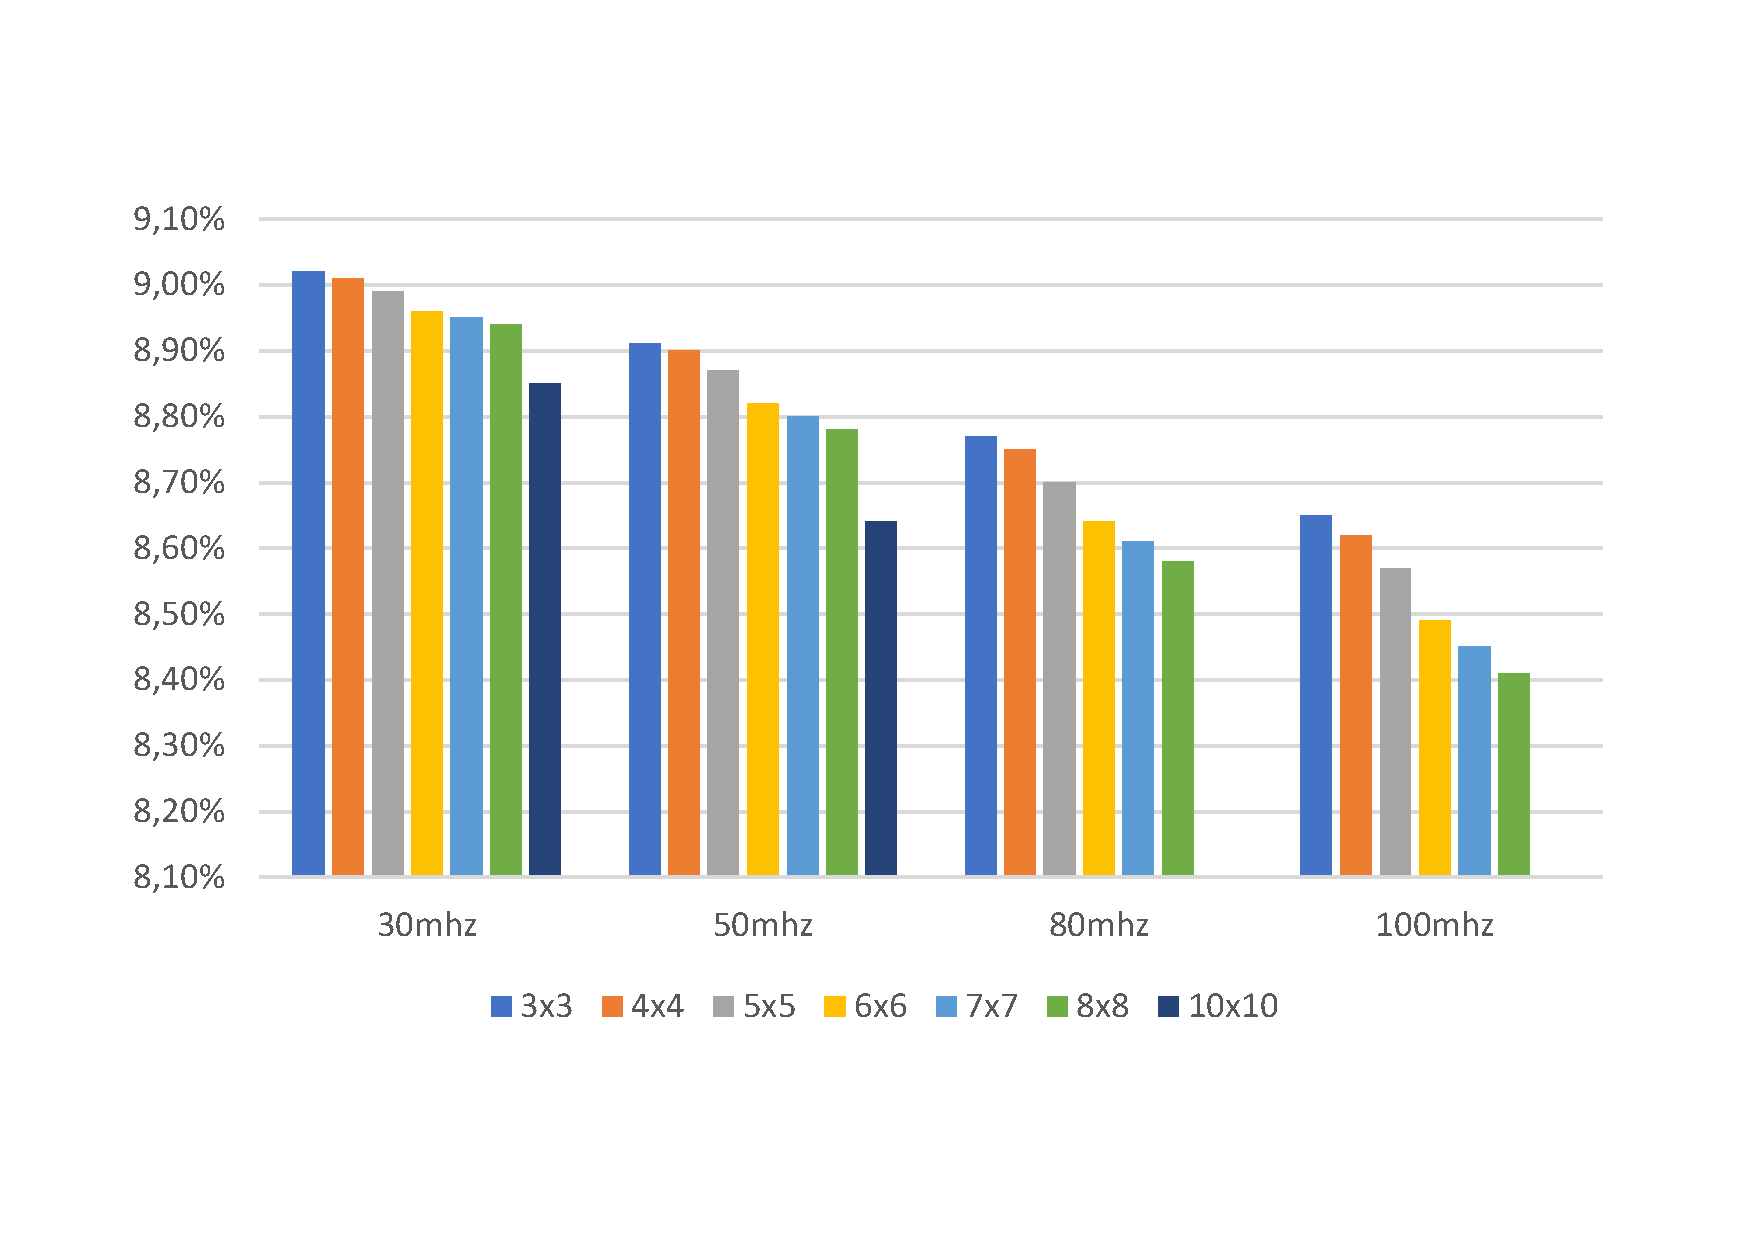
\includegraphics[scale=0.5,angle=0]{./figure/graphs/power_plstatic_int32_freq.pdf}
\caption{Post Implementation Static Power Consumption Programmable logic for integer 32 PEs }
\label{fig:staticpowint32}
\end{figure}
\begin{figure}[!htbp]
\centering
\captionsetup{justification=centering}
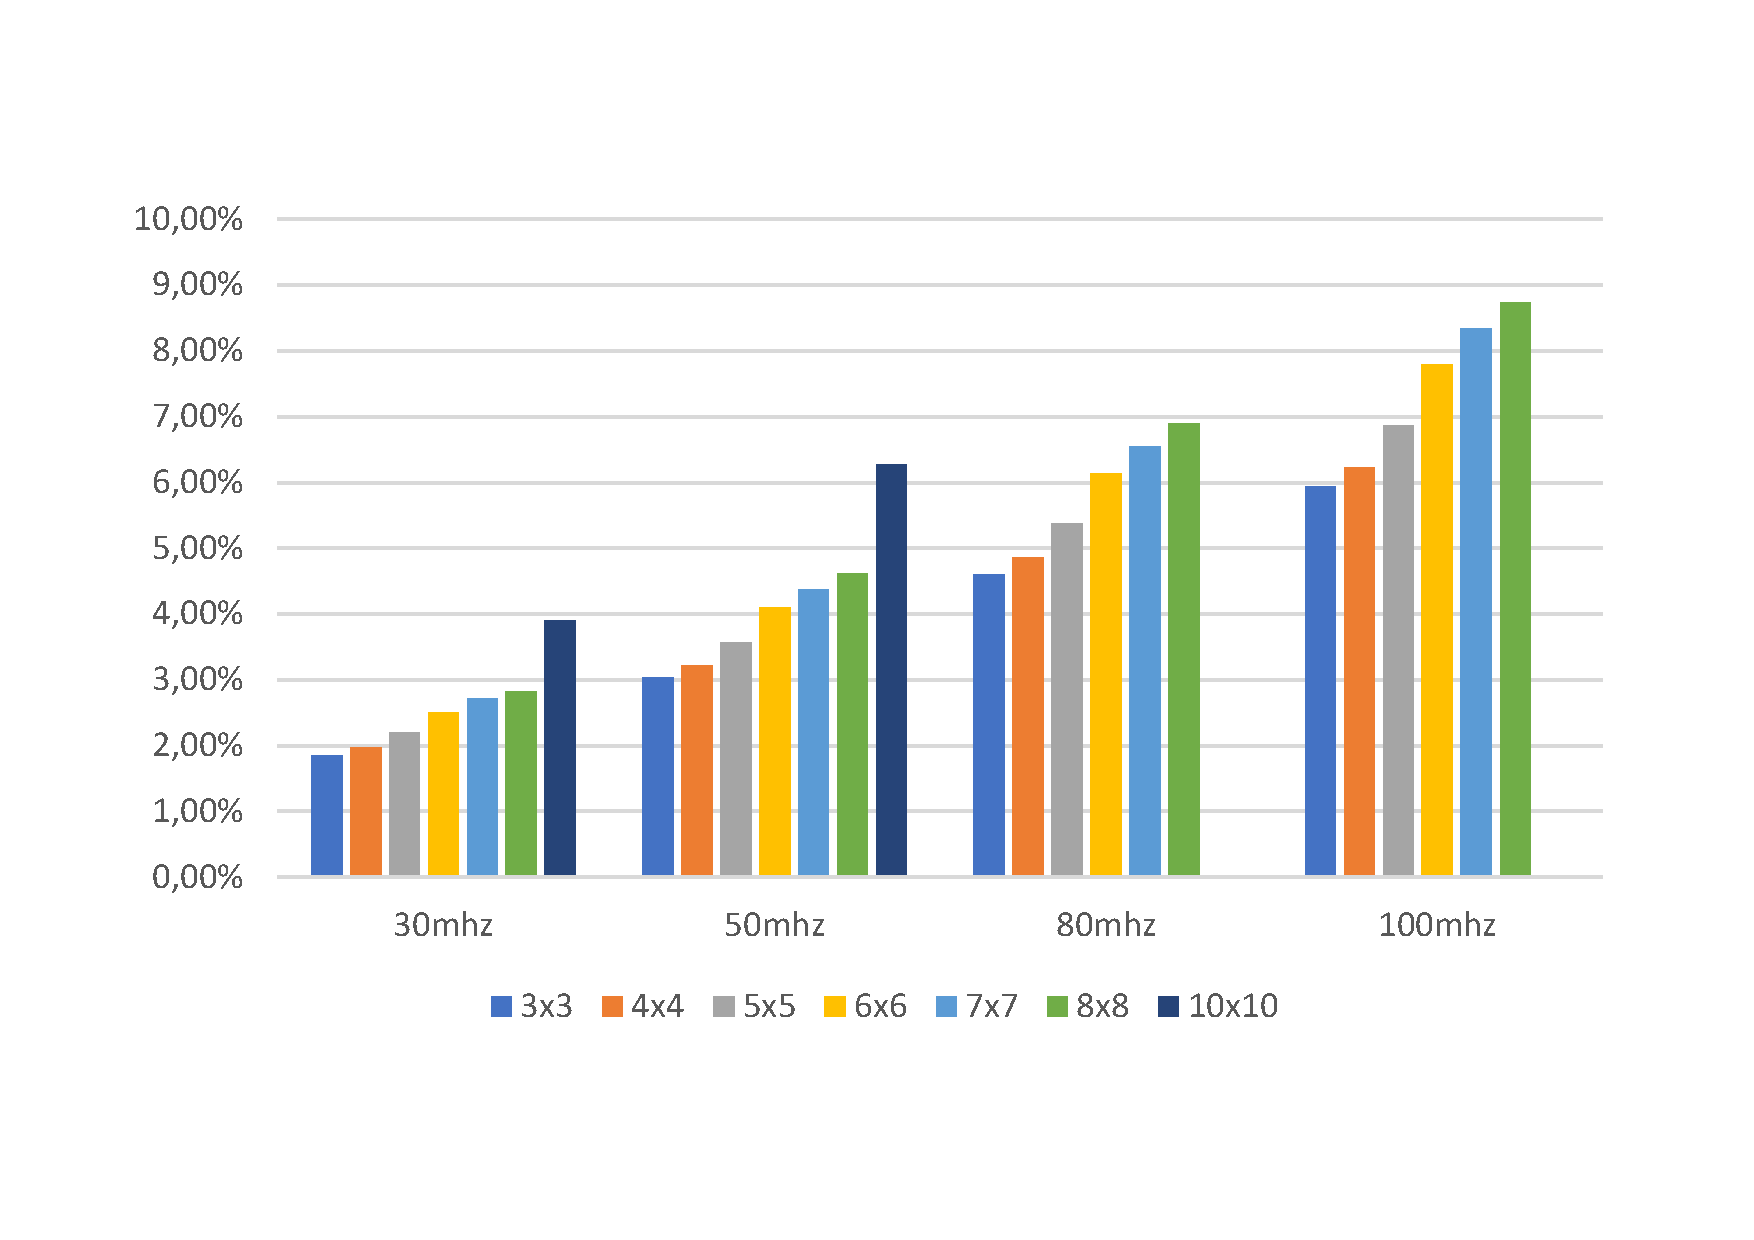
\includegraphics[scale=0.5,angle=0]{./figure/graphs/power_pldyn_int32_freq.pdf}
\caption{Post Implementation Dynamic Power Consumption per Programmable logic with integer 32 PEs}
\label{fig:dynpowint32}
\end{figure}
\begin{figure}[!htbp]
\centering
\captionsetup{justification=centering}
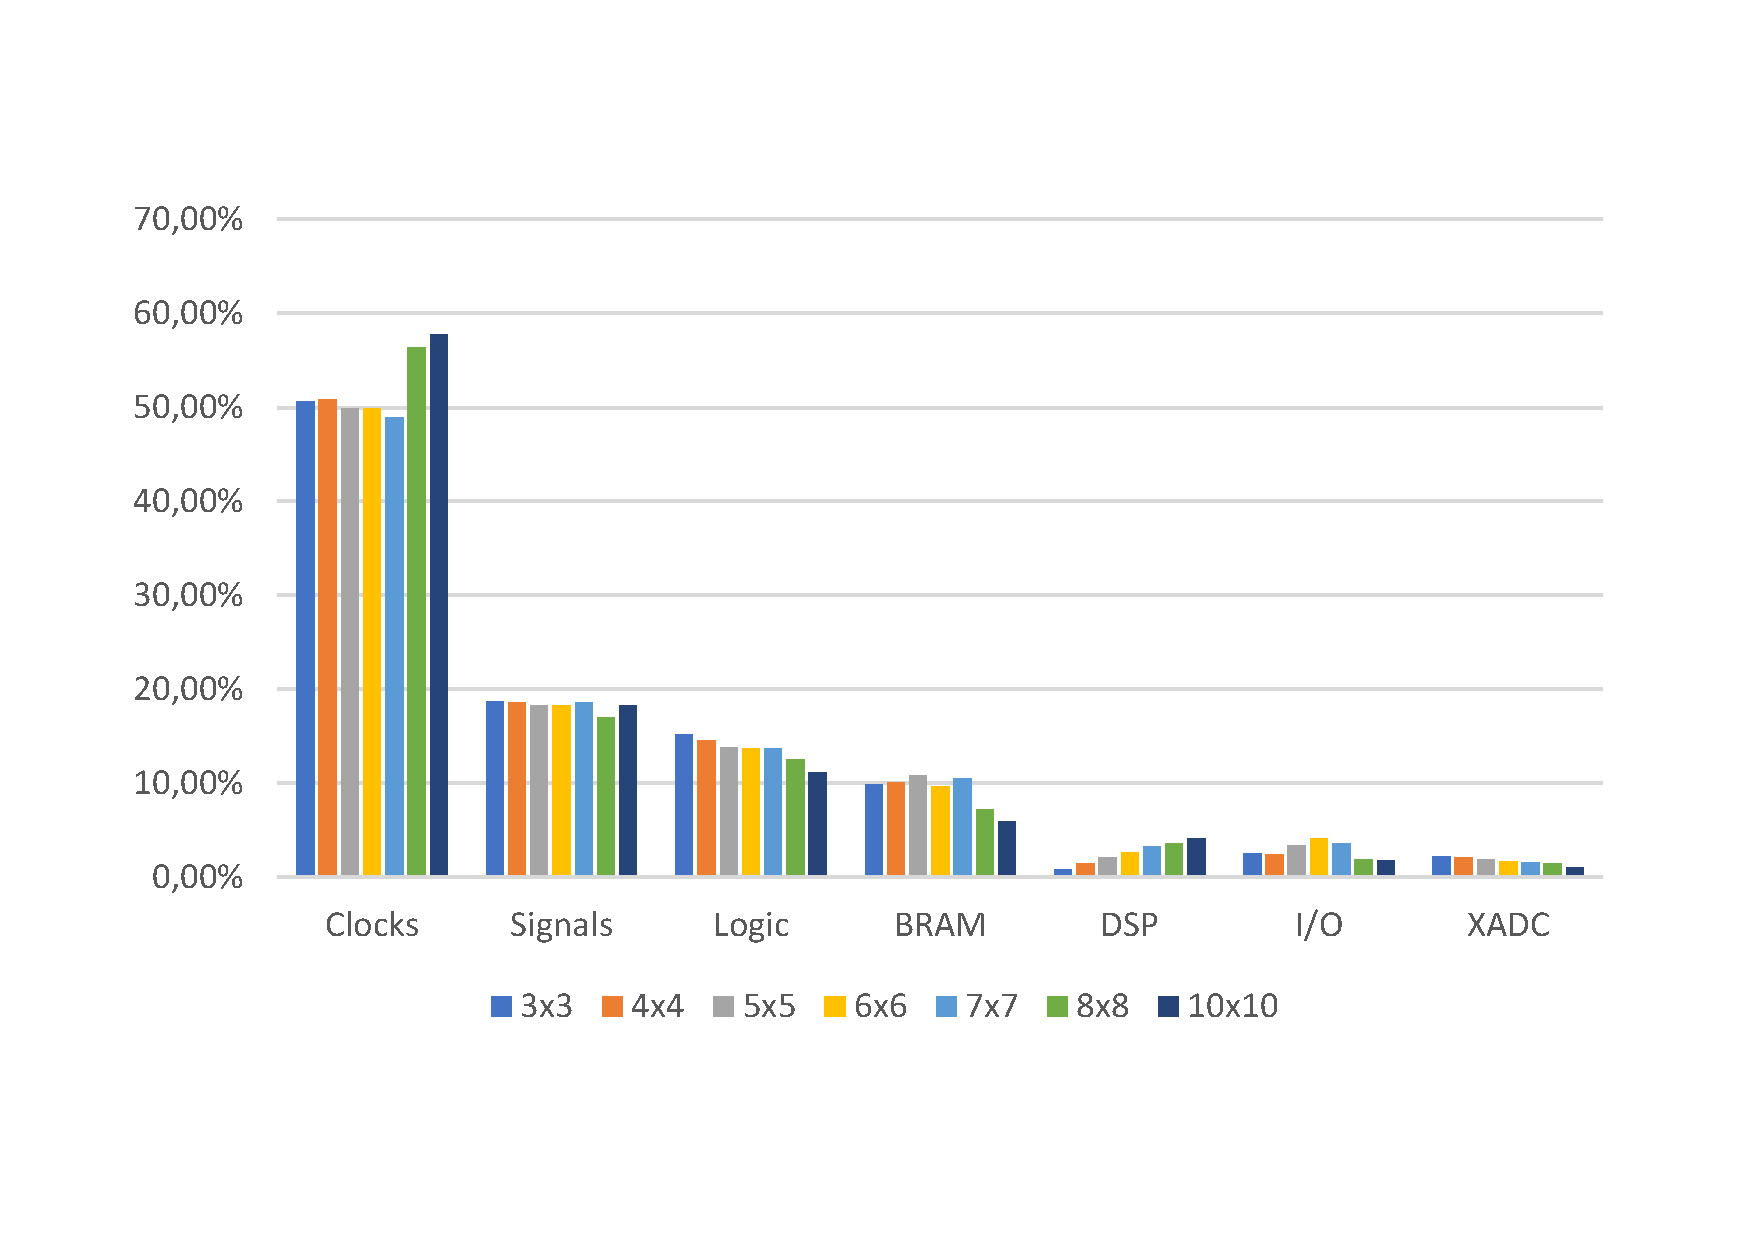
\includegraphics[scale=0.6,angle=0]{./figure/graphs/power_pldyn_div_int32_freq_30mhz.pdf}
\caption{Post Implementation Dynamic Power Consumption per entities in Programmable Logic with a clock frequency of 30 MHz and integer 32 PEs}
\label{fig:dynpowint32ent30}
\end{figure}
\begin{figure}[!htbp]
\centering
\captionsetup{justification=centering}
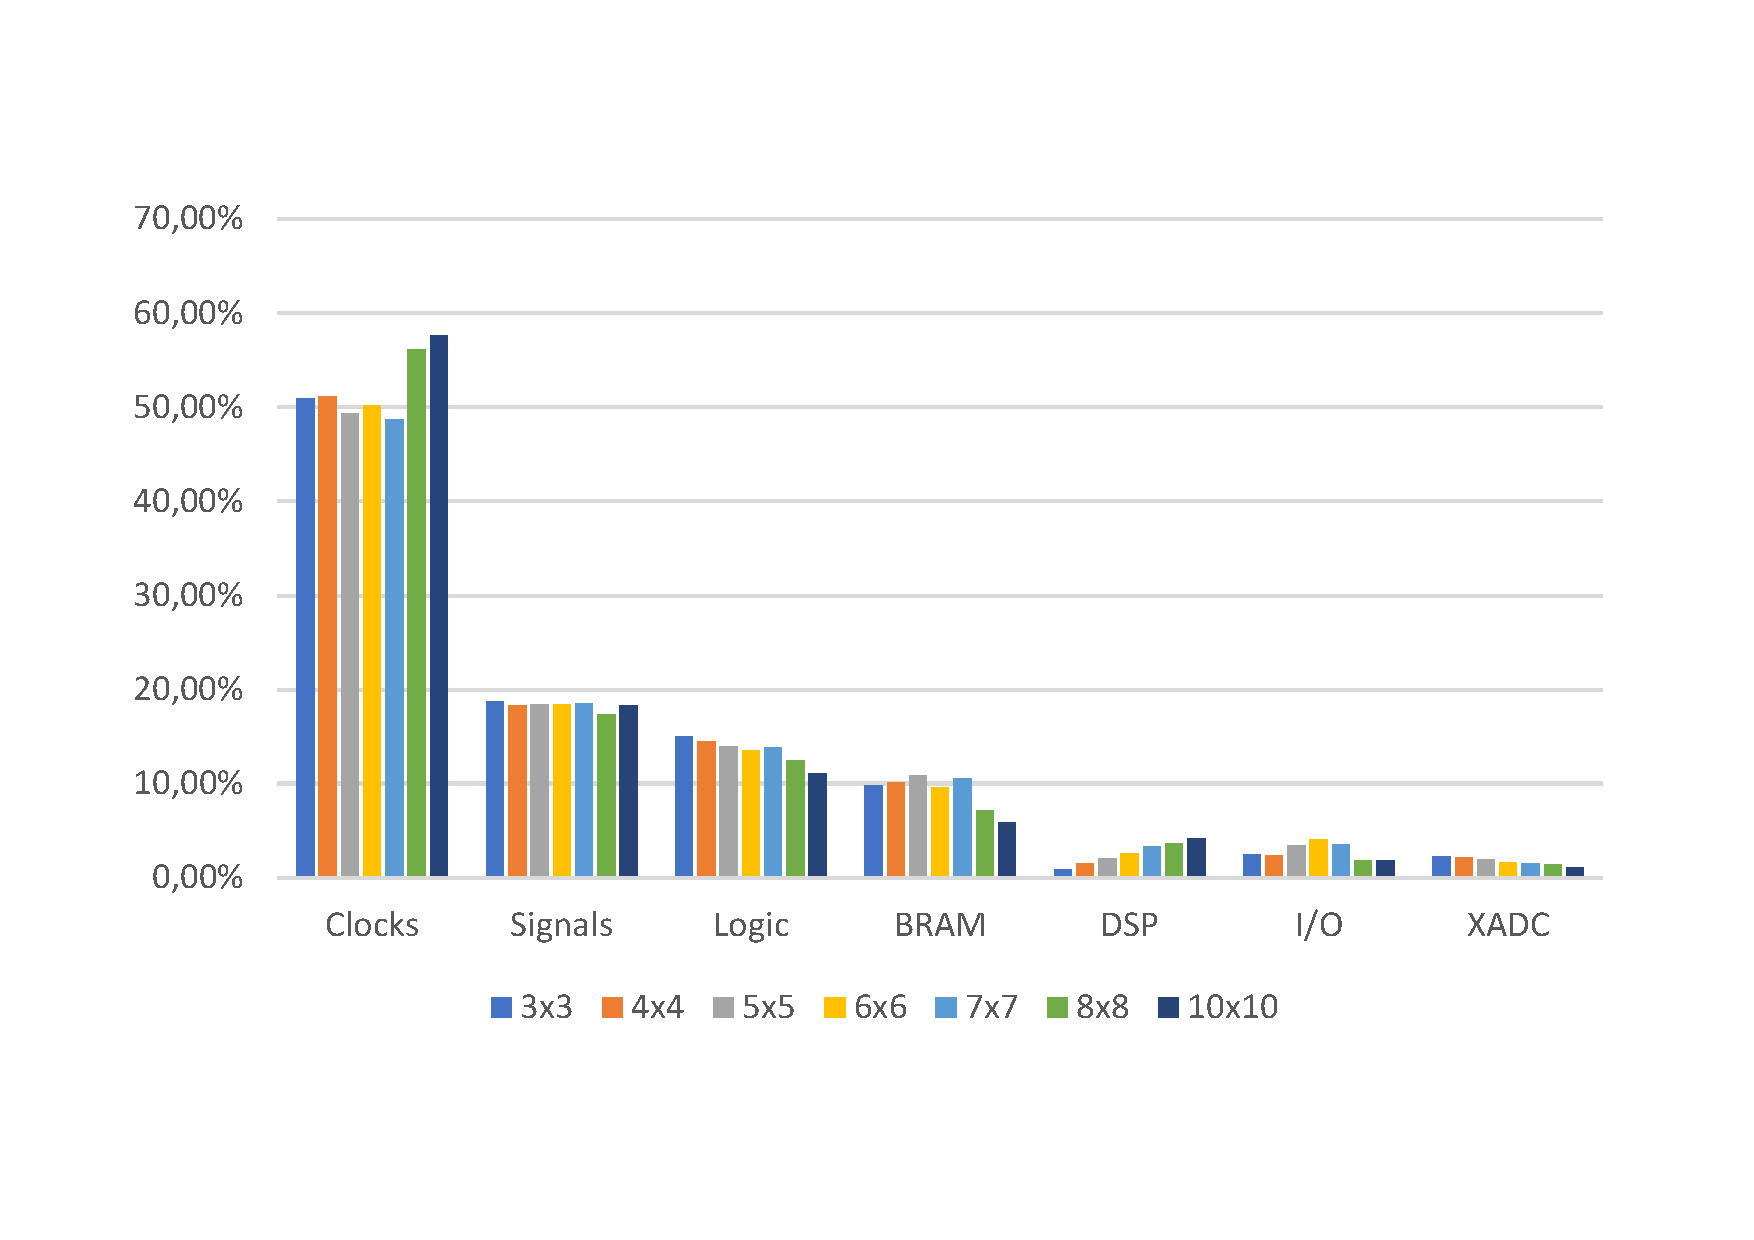
\includegraphics[scale=0.6,angle=0]{./figure/graphs/power_pldyn_div_int32_freq_50mhz.pdf}
\caption{Post Implementation Dynamic Power Consumption per entities in Programmable Logic with a clock frequency of 50 MHz and integer 32 PEs}
\label{fig:dynpowint32ent50}
\end{figure}
\begin{figure}[!htbp]
\centering
\captionsetup{justification=centering}
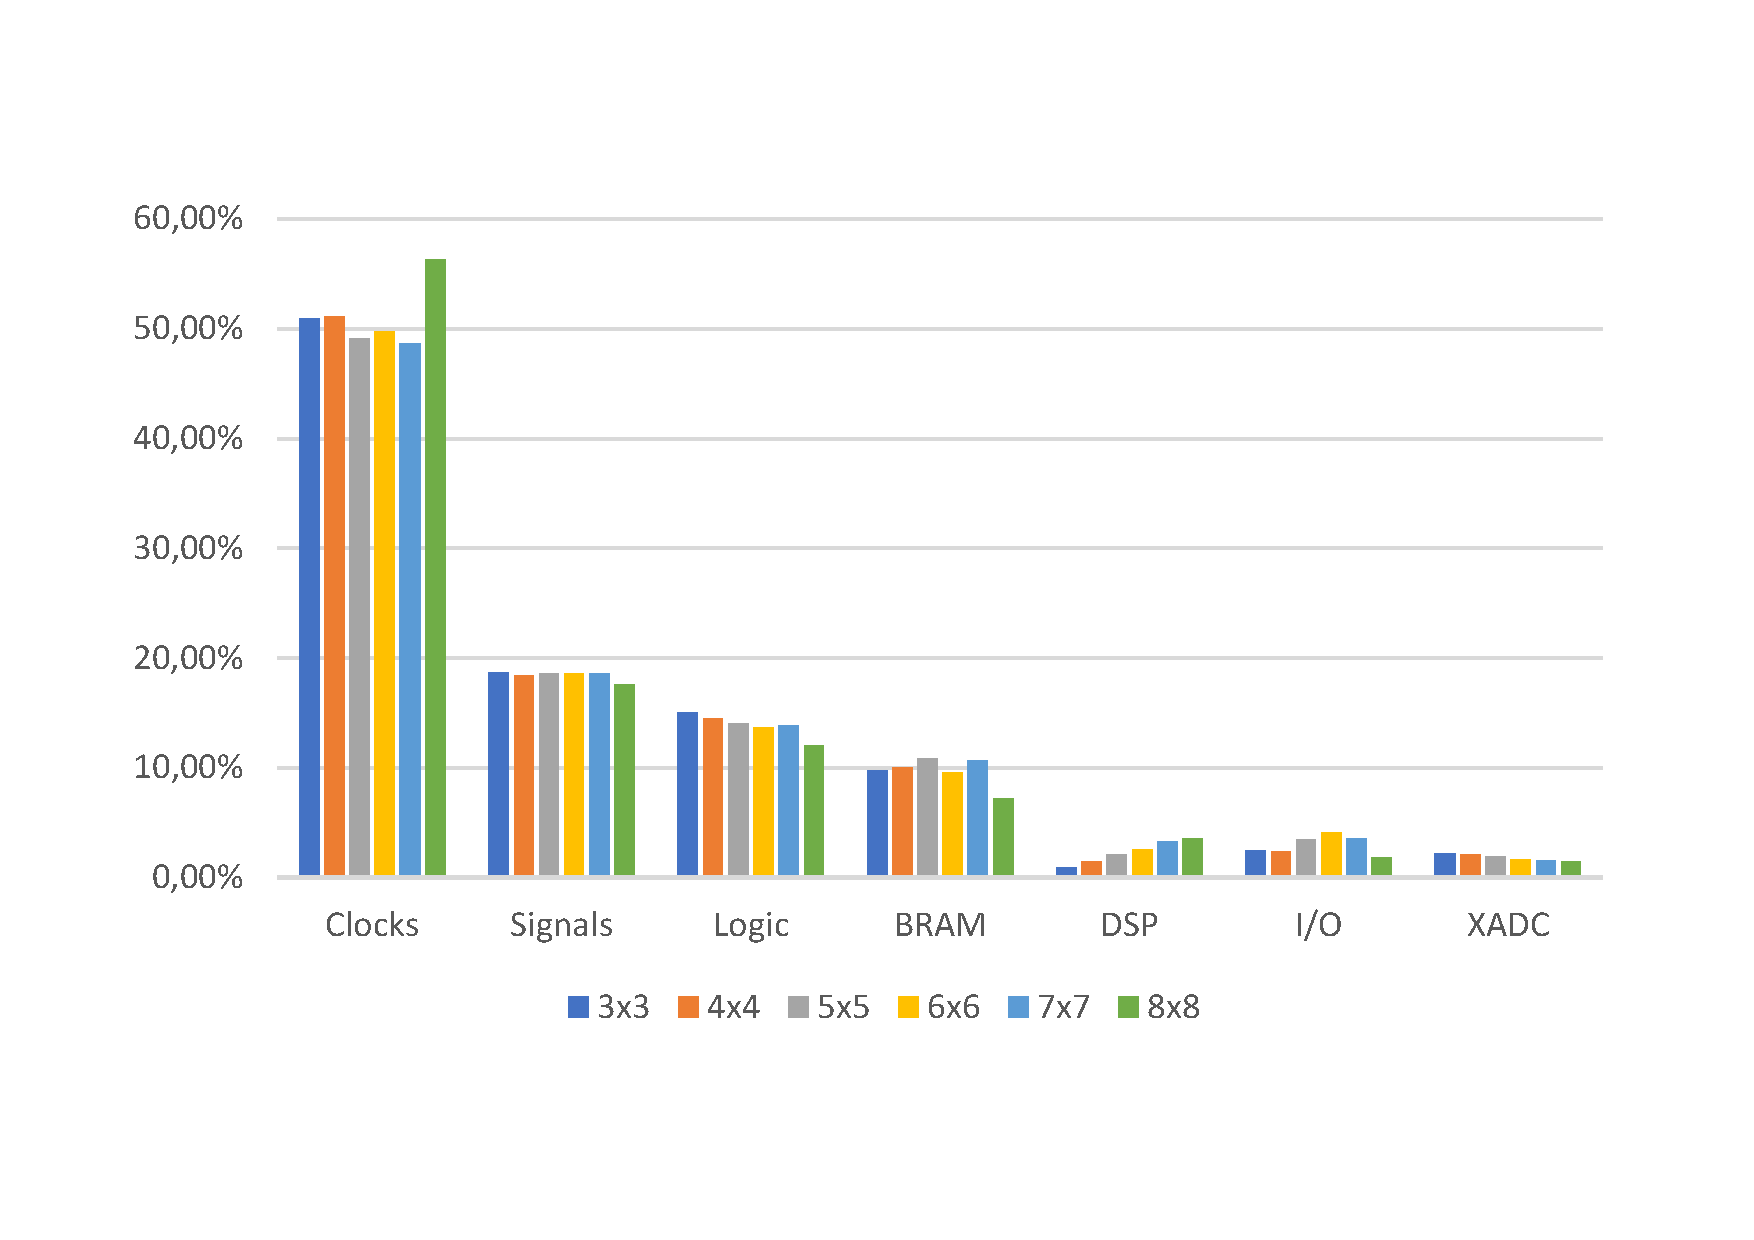
\includegraphics[scale=0.6,angle=0]{./figure/graphs/power_pldyn_div_int32_freq_80mhz.pdf}
\caption{Post Implementation Dynamic Power Consumption per entities in Programmable Logic with a clock frequency of 80 MHz and integer 32 PEs}
\label{fig:dynpowint32ent80}
\end{figure}
\begin{figure}[!htbp]
\centering
\captionsetup{justification=centering}
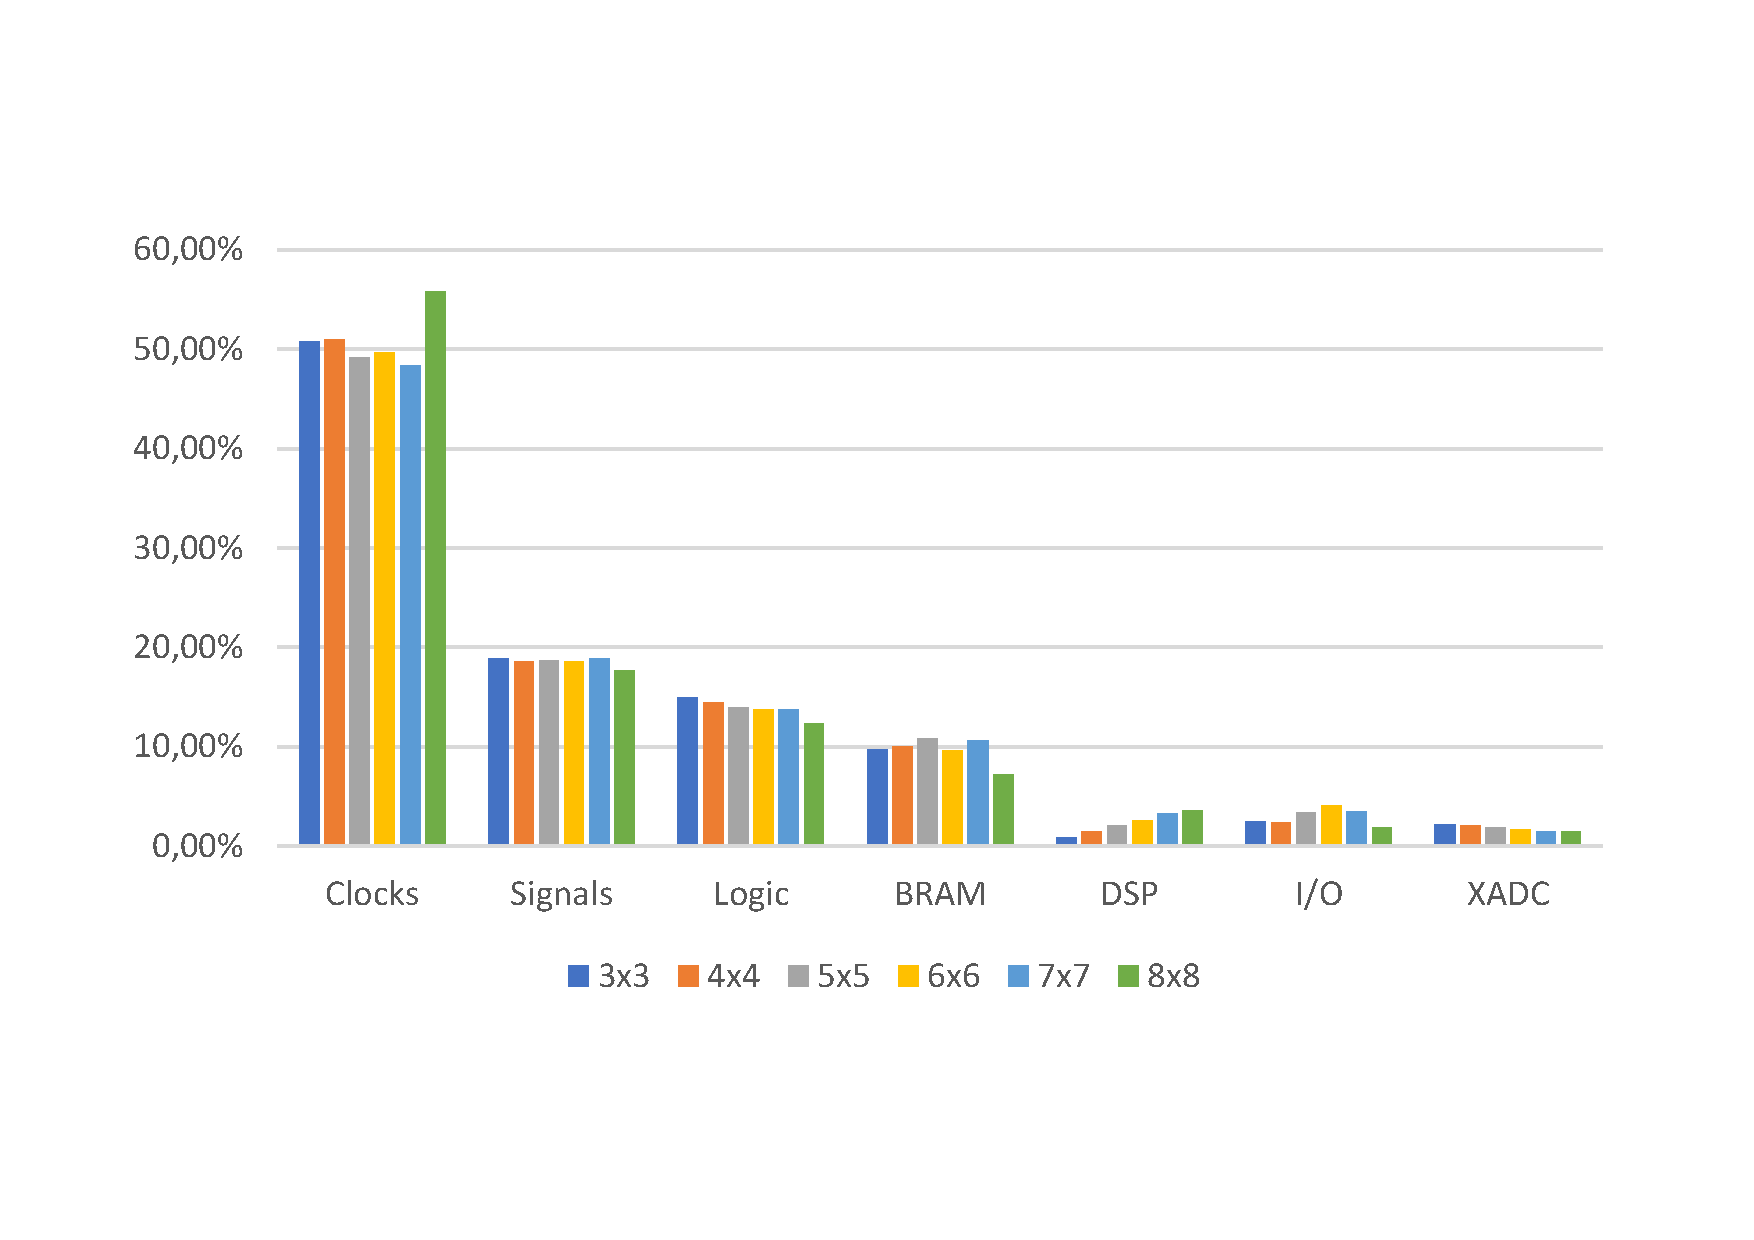
\includegraphics[scale=0.6,angle=0]{./figure/graphs/power_pldyn_div_int32_freq_100mhz.pdf}
\caption{Post Implementation Dynamic Power Consumption per entities in Programmable Logic with a clock frequency of 100 MHz and integer 32 PEs}
\label{fig:dynpowint32ent100}
\end{figure}

It is worth to mention the power consumed by the DSP entities, comparing to integer 8 and 16 PEs, is bigger. The main reason is that there is no more one to one mapping between PEs and DSP entities.

\item Integer 64:
\begin{figure}[!htbp]
\centering
\captionsetup{justification=centering}
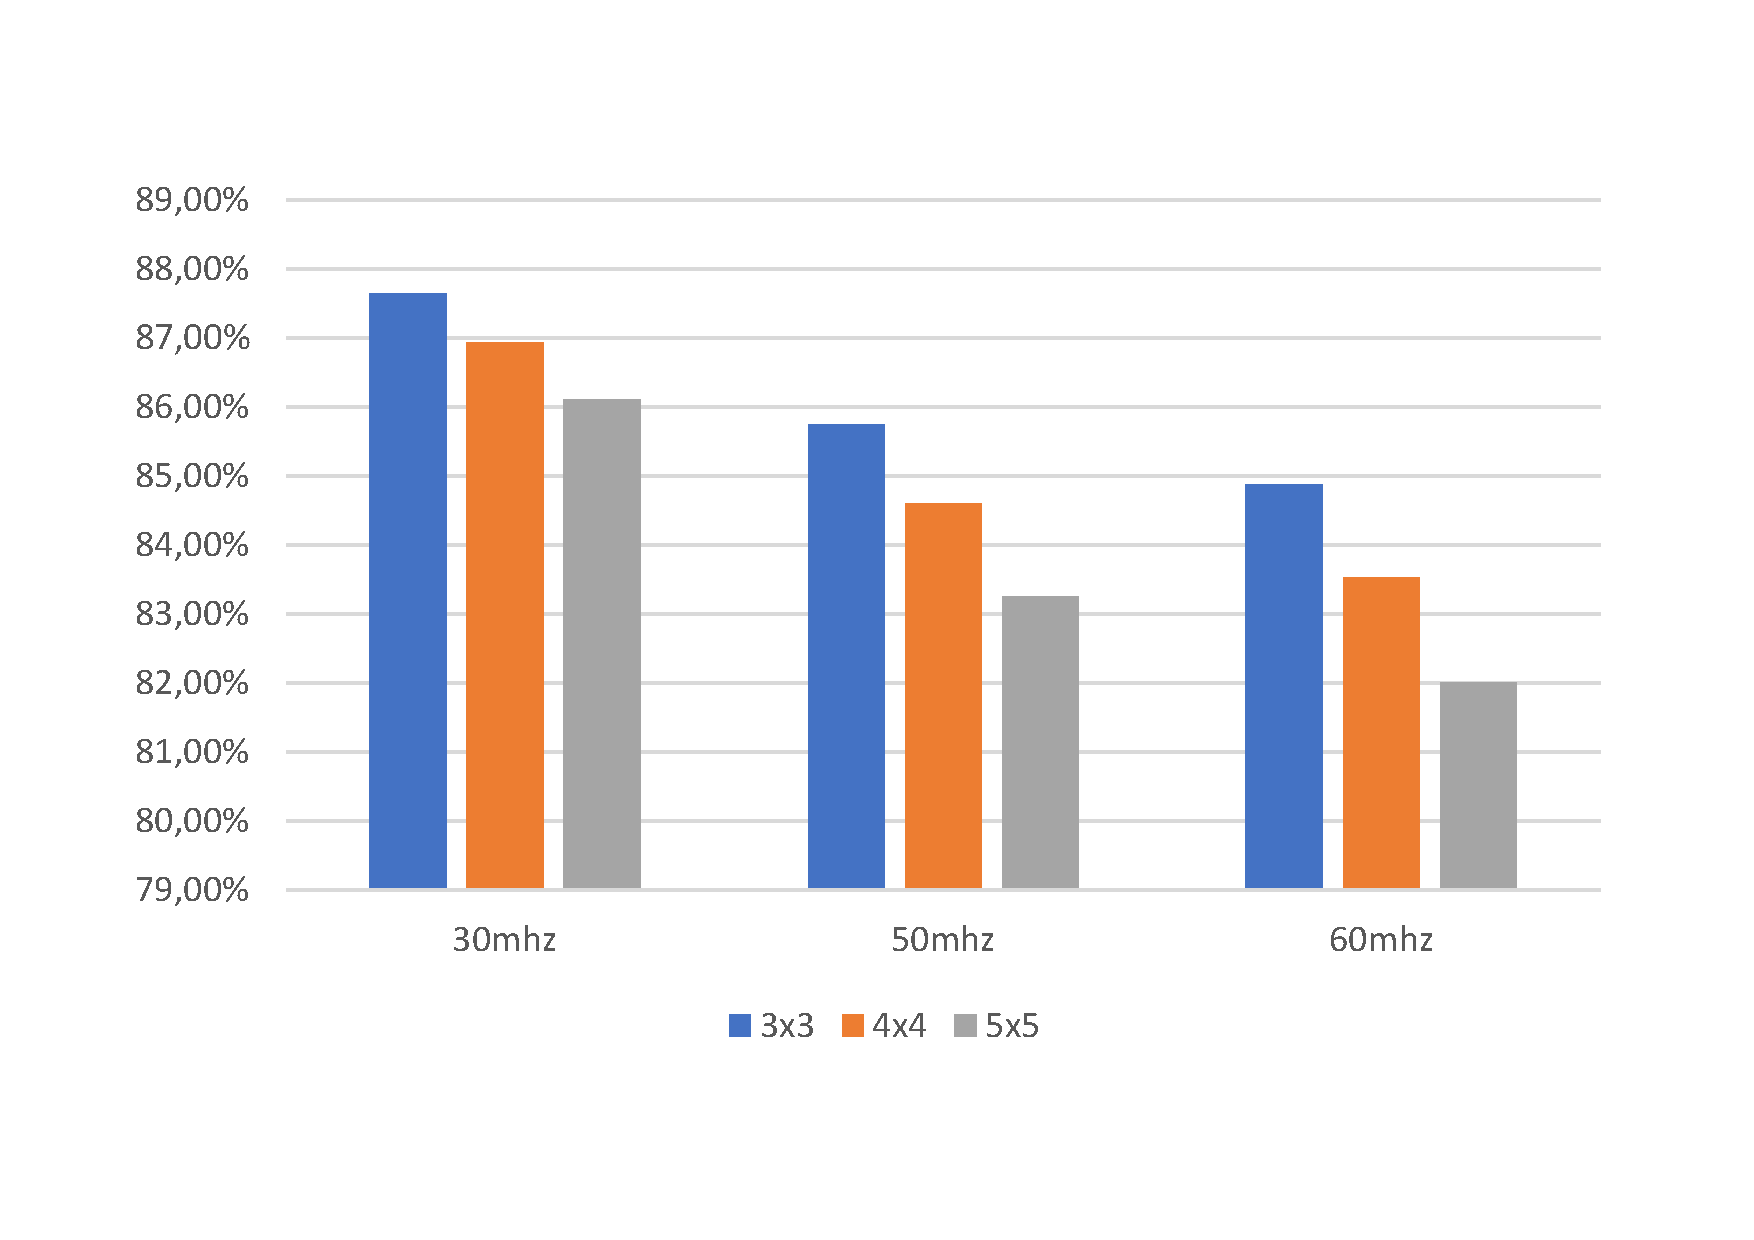
\includegraphics[scale=0.5,angle=0]{./figure/graphs/power_ps_int64_freq.pdf}
\caption{Post Implementation Power Consumption of Processing System for integer 64 PEs}
\label{fig:powint64}
\end{figure}
\begin{figure}[!htbp]
\centering
\captionsetup{justification=centering}
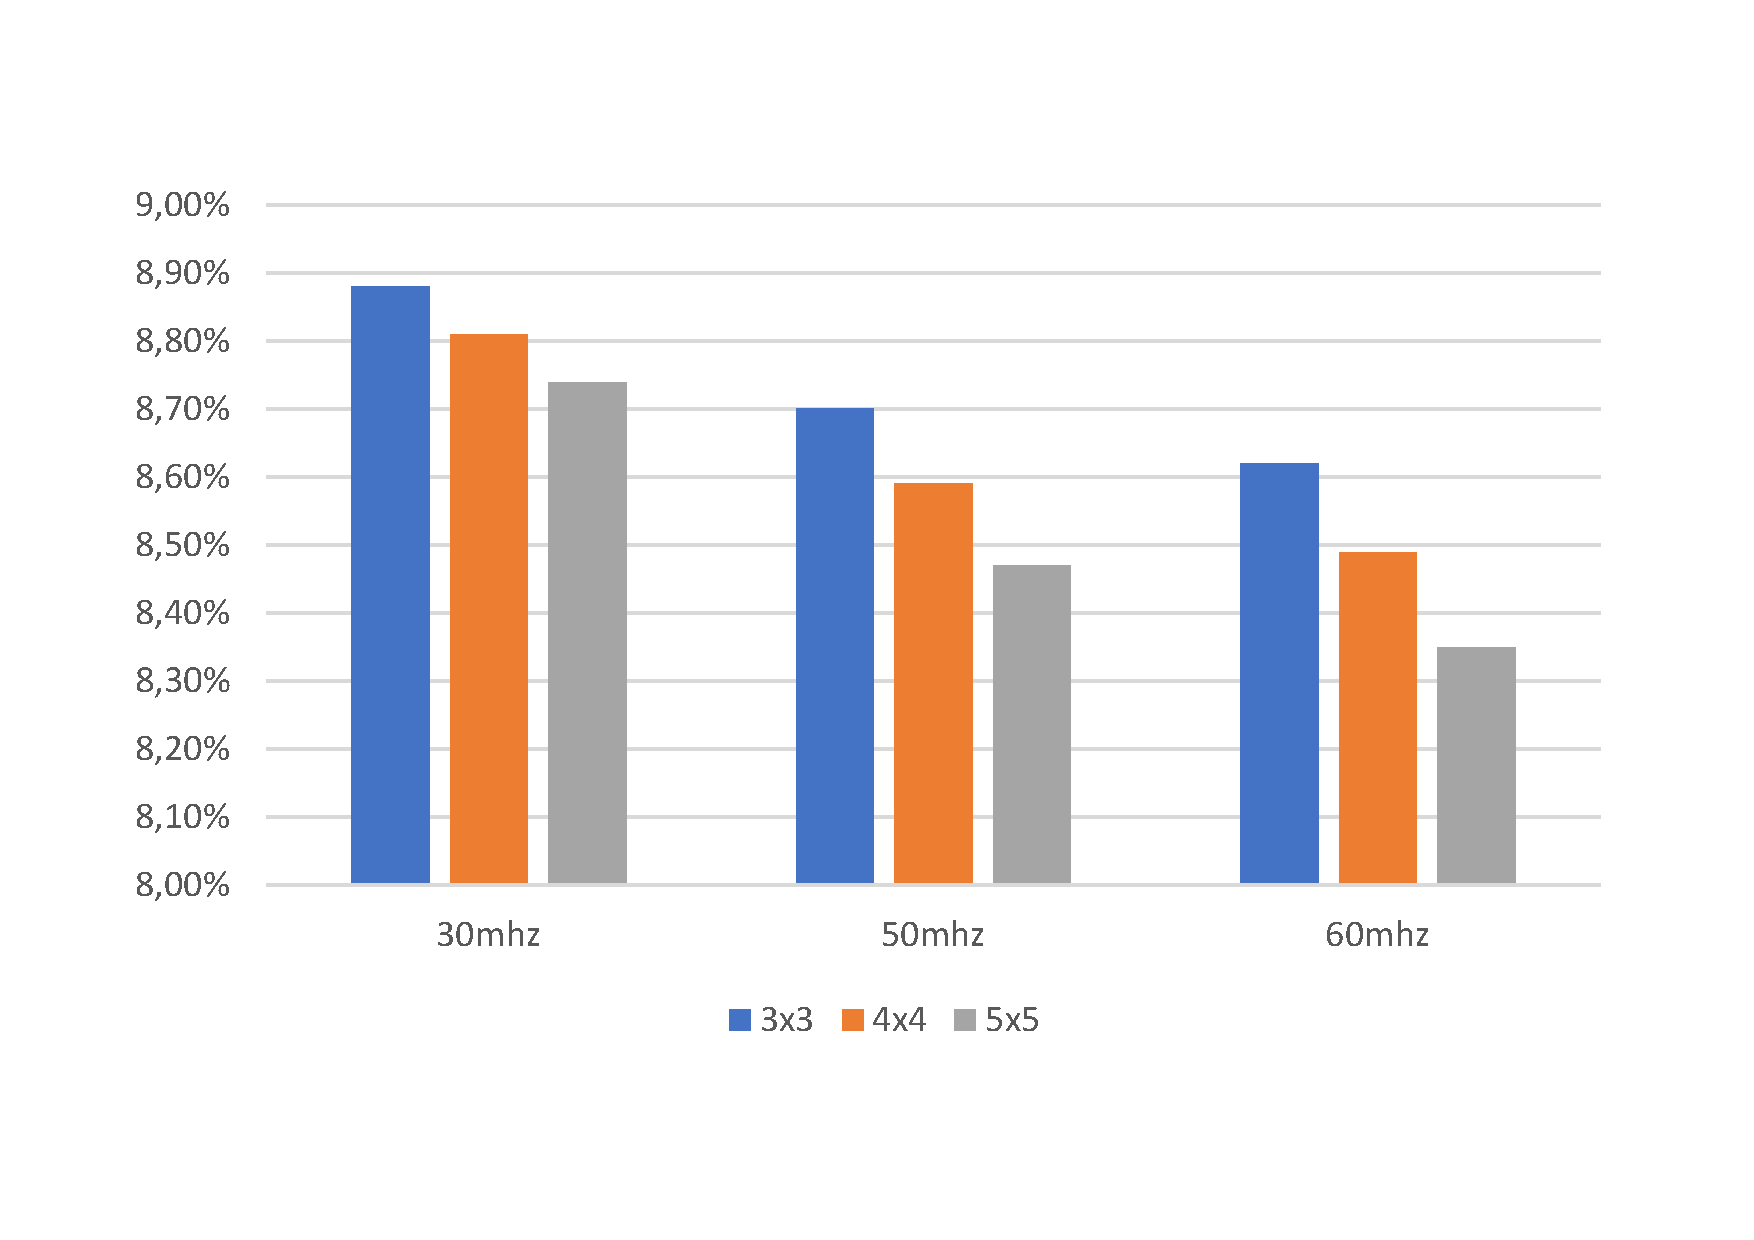
\includegraphics[scale=0.5,angle=0]{./figure/graphs/power_plstatic_int64_freq.pdf}
\caption{Post Implementation Static Power Consumption Programmable logic for integer 64 PEs }
\label{fig:staticpowint64}
\end{figure}
\begin{figure}[!htbp]
\centering
\captionsetup{justification=centering}
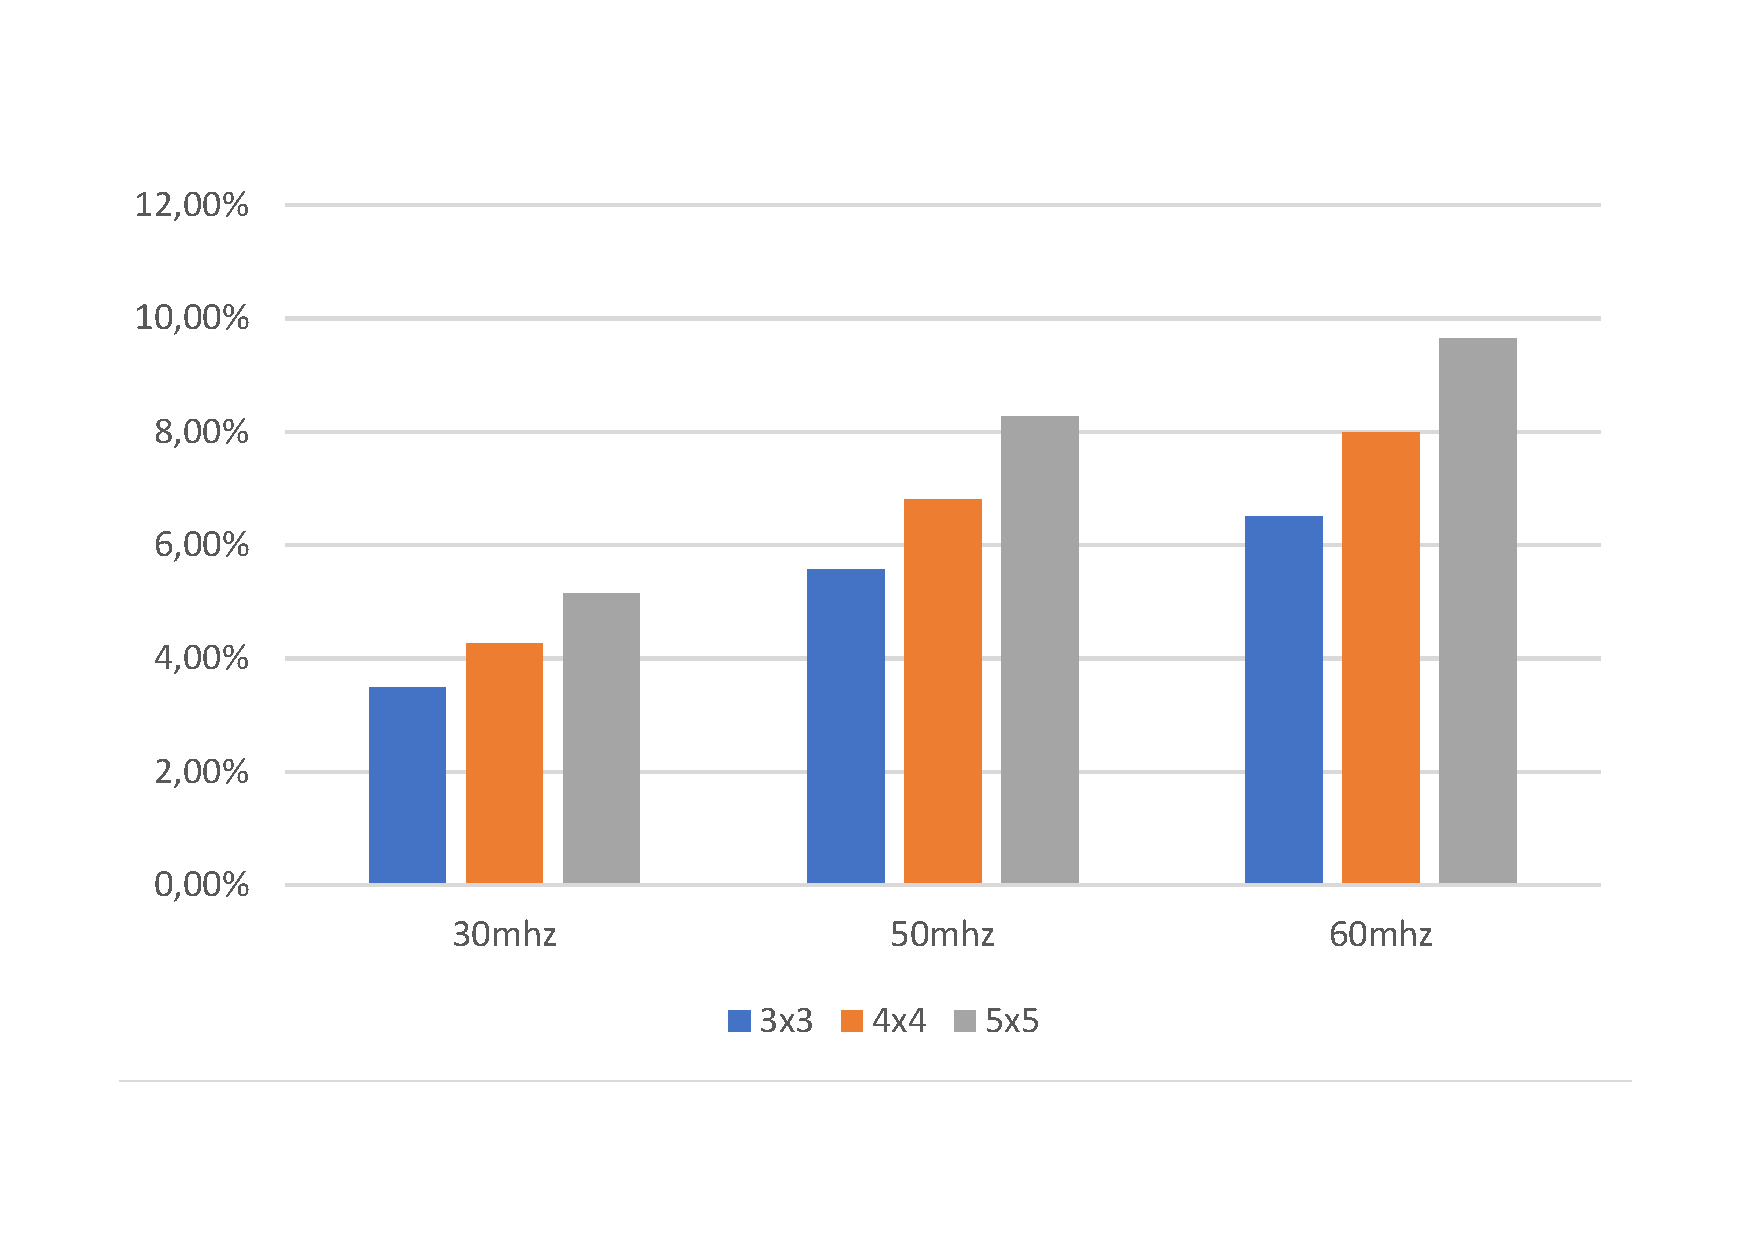
\includegraphics[scale=0.5,angle=0]{./figure/graphs/power_pldyn_int64_freq.pdf}
\caption{Post Implementation Dynamic Power Consumption per Programmable logic with integer 64 PEs}
\label{fig:dynpowint64}
\end{figure}
\begin{figure}[!htbp]
\centering
\captionsetup{justification=centering}
\includegraphics[scale=0.6,angle=0]{./figure/graphs/power_pldyn_div_int64_freq_30mhz.pdf}
\caption{Post Implementation Dynamic Power Consumption per entities in Programmable Logic with a clock frequency of 30 MHz and integer 64 PEs}
\label{fig:dynpowint64ent30}
\end{figure}
\begin{figure}[!htbp]
\centering
\captionsetup{justification=centering}
\includegraphics[scale=0.6,angle=0]{./figure/graphs/power_pldyn_div_int64_freq_50mhz.pdf}
\caption{Post Implementation Dynamic Power Consumption per entities in Programmable Logic with a clock frequency of 50 MHz and integer 64 PEs}
\label{fig:dynpowint64ent50}
\end{figure}
\begin{figure}[!htbp]
\centering
\captionsetup{justification=centering}
\includegraphics[scale=0.6,angle=0]{./figure/graphs/power_pldyn_div_int64_freq_60mhz.pdf}
\caption{Post Implementation Dynamic Power Consumption per entities in Programmable Logic with a clock frequency of 60 MHz and integer 64 PEs}
\label{fig:dynpowint64ent60}
\end{figure}

As mentioned in the Utilization chapter, the PEs on 64 bit integer are using 14 DSP entities (for having the possibility to compute vectorized operations on data). Therefore, this heavy utilization per PEs is impacting also the power consumed by the DSPs but as it can be seen in Figures fromi \ref{fig:dynpowint64ent30} to \ref{fig:dynpowint64ent60}.
\newpage
\item Brain floating point 16:
\begin{figure}[!htbp]
\centering
\captionsetup{justification=centering}
\includegraphics[scale=0.5,angle=0]{./figure/graphs/power_bfp16_freq.pdf}
\caption{Post Implementation Power Consumption for bfp16 PEs}
\label{fig:powbfp16}
\end{figure}
\begin{figure}[!htbp]
\centering
\captionsetup{justification=centering}
\includegraphics[scale=0.5,angle=0]{./figure/graphs/power_pldyn_div_bfp16_freq_30mhz.pdf}
\caption{Post Implementation Dynamic Power Consumption per entities in Programmable Logic with a clock frequency of 30 MHz and bfp16 PEs}
\label{fig:dynpowintbfp16ent30}
\end{figure}
\newpage
\item Floating point 32: 
\begin{figure}[!htbp]
\centering
\captionsetup{justification=centering}
\includegraphics[scale=0.47,angle=0]{./figure/graphs/power_fp32_freq.pdf}
\caption{Post Implementation Power Consumption for fp32 PEs}
\label{fig:powfp32}
\end{figure}
\begin{figure}[!htbp]
\centering
\captionsetup{justification=centering}
\includegraphics[scale=0.47,angle=0]{./figure/graphs/power_pldyn_div_fp32_freq_30mhz.pdf}
\caption{Post Implementation Dynamic Power Consumption per entities in Programmable Logic with a clock frequency of 30 MHz and fp32 PEs}
\label{fig:dynpowintfp32ent30}
\end{figure}\\
For the bfp16 and fp32 it can be seen that the majority of the power is consumed by the interconnections and the logic. Mainly, because the PEs are implemented in logic.
\end{itemize}
\newpage
Until now, the focus has been on how much the single entities and the different type of power were impacting the total power consumption. It is also worth to compare the absolute values for different data precision, as in the Figure \ref{fig:dynpowcomparisonent3033}.\\
\begin{figure}[!htbp]
\centering
\captionsetup{justification=centering}
\includegraphics[scale=0.5,angle=0]{./figure/graphs/power_dyn_comparison_pes_30mhz_3x3.pdf}
\caption{Comparison of Post Implementation Dynamic Power Consumption per entities in Programmable Logic with a clock frequency of 30 MHz and a MXU 3x3}
\label{fig:dynpowcomparisonent3033}
\end{figure}\\
As it is very well known from literature and it has also been evident from the other figures and observations, the power consumption per entities grows with the increase of the bitwidth (in the case of integer) and complexity (in the case of floating point).\\
The power consumed by the DSPs (entities in which the integer PEs are implemented in) is negligible for the integer 8 and 16 while it starts to grow slowly using the integer 32 but it explodes with the 64 bit PEs. The high utilization of those PEs leads also to a huge impact in their power consumption.

\todo{should we add the runtime measurement?}

\newpage

\section{Throughput}
According to the definition, the Throughput is the amount of units of information a system can process in a given time. As said that, for the designed accelerator, it results to be equal to the number of rows into the Matrix Multiplication Unit. Normalizing this value with the clock frequency, it results to be constant for all the data type and frequencies.
\begin{figure}[!htbp]
\centering
\captionsetup{justification=centering}
\includegraphics[scale=0.45,angle=0]{./figure/graphs/roofline.pdf}
\caption{Roofline model of the accelerator with a MXU size of 8x8}
\label{fig:roofline}
\end{figure}

The theoretical throughput given by the roofline model (Figure \label{fig:roofline}) and it is equal to the number of rows in the matrix multiplication unit. The assumption is that enough data are provided to the accelerator in order to have all the Processing Elements working with useful data, if the latter is not meet the throughput goes down.
In Figure \label{fig:roofline} the different slopes for different data width are representing the different number of internal memory accessess in order to retrieve data for all the Processing Elements.\\

The throughput can be further increased in the 64-bitwidth configuration of the Processing Elements. As already mentioned, those 64-bit units are able to compute vectorized instructions and therefore increase the number of computation per cycle. However, this comes with the overhead of more memory accesses as it can be apprecieted in the \label{fig:rooflinevect}.

\begin{figure}[!htbp]
\centering
\captionsetup{justification=centering}
\includegraphics[scale=0.45,angle=0]{./figure/graphs/roofline_vectorized.pdf}
\caption{Roofline model of the accelerator with a MXU size of 8x8 and vectorized PEs}
\label{fig:rooflinevect}
\end{figure}
 \newpage
 
\section{Latency}
In a real time application, the most important factor is the latency, the execution time of a task.
In this case the latency is measured as average of the execution time of a Neural Network model for different platforms. In addition, the execution of the models, on the target, in the configuration \textit{CPU+accelerator} is done with different clock frequencies and data type in the Programmable Logic, and as consequence a different overall latency (and power consumption).\\
In the following tables, the execution type for different data type and model is presented (with a fixed clock frequency of the accelerator at 50 MHz).
\begin{center}
\begin{table}[!htbp]
\centering
\captionsetup{justification=centering}
\begin{tabular}{ |p{2.5cm}||p{2.5cm}|p{2.5cm}|p{2.5cm}|p{2.5cm}| }
\hline
Model & CPU (host)\protect\footnotemark[1] & GPU(host)\protect\footnotemark[2] & CPU(Pynq Z2 board)\protect\footnotemark[3] & CPU(Pynq Z2 board) + accelerator \\
\hline
MNIST & 0.3 ms & 5.7 ms & 2.9 ms  &  509 ms 
\\
\hline
Cifar 10& 20 ms & 22 ms& 160 ms & 13356 ms\\
\hline
\end{tabular}
\caption{Execution Time for different platform and model, integer 8}
\label{table:moplatint8}
\end{table}
\end{center}

\begin{center}
\begin{table}[!htbp]
\centering
\captionsetup{justification=centering}
\begin{tabular}{ |p{2.5cm}||p{2.5cm}|p{2.5cm}|p{2.5cm}|p{2.5cm}| }
\hline
Model & CPU (host)\protect\footnotemark[1] & GPU(host)\protect\footnotemark[2] & CPU(Pynq Z2 board)\protect\footnotemark[3] & CPU(Pynq Z2 board) + accelerator \\
\hline
MNIST & 0.3 ms & 5.7 ms & 2.9 ms  &  503 ms
\\
\hline
Cifar 10& 20 ms & 22 ms& 160 ms & 13178 ms 
\\
\hline
\end{tabular}
\caption{Execution Time for different platform and model, integer 16}
\label{table:moplatint16}
\end{table}
\end{center}
\begin{center}
\begin{table}[!htbp]
\centering
\captionsetup{justification=centering}
\begin{tabular}{ |p{2.5cm}||p{2.5cm}|p{2.5cm}|p{2.5cm}|p{2.5cm}| }
\hline
Model & CPU (host)\protect\footnotemark[1] & GPU(host)\protect\footnotemark[2] & CPU(Pynq Z2 board)\protect\footnotemark[3] & CPU(Pynq Z2 board) + accelerator \\
\hline
MNIST & 0.3 ms & 5.7 ms & 2.9 ms  & 496.9 ms
\\
\hline
Cifar 10& 20 ms & 22 ms& 160 ms & 13218 ms
\\
\hline
\end{tabular}
\caption{Execution Time for different platform and model, integer 32}
\label{table:moplatint32}
\end{table}
\end{center}

\footnotetext[1]{Intel i7-6700HQ, 2.60 Ghz}
\footnotetext[2]{NVIDIA, GeForce GTX960M, 1.176 Ghz }
\footnotetext[3]{Arm dual-core Cortex-A9, 650 MHz }
Looking at the previous tables, the latency for different data precision it is not changing. This is due to the hardware structure, the Matrix Multiplication Unit is build in such a way that the latency between the one operation and the next one is always of 3 clock cycles (for integer operations).\\\\
It is worth to analyze and reason about the increase in the latency in the configuration with the accelerator, since one of the main goal was to reduce the latency time. \\
Focusing on the following Figure:
\begin{figure}[!htbp]
\centering
\captionsetup{justification=centering}
\includegraphics[scale=0.55,angle=0]{./figure/graphs/latency_subdivision_mnist.pdf}
\caption{Total Execution time of Invoke method (left) in the configuration with accelerator and MNIST model}
\label{fig:totexecmnist}
\end{figure}

\begin{figure}[!htbp]
\centering
\captionsetup{justification=centering}
\includegraphics[scale=0.55,angle=0]{./figure/graphs/latency_subdivision_cifar10.pdf}
\caption{Total Execution time of Invoke method (left) in the configuration with accelerator and Cifar10 model}
\label{fig:totexeccifar10}
\end{figure}
\newpage
As it has been mentioned before, the most compute intensive part is always the Convolution operations. Introducing the hardware accelerator and its library comes with several overheads as it can be seen in Figures \ref{fig:totexecmnist} and \ref{fig:totexeccifar10}:\\
\begin{itemize}
\item Data exchange between C and python: the accelerator library has been developed in Python code with the C interface to Tensorflow Lite. This means that every matrix (input, output and weight) is copied to the python sublayer for further processing. Migrating all the accelerator library into C code will remove this overhead.
\item Hardware execution time and rebuilding of output matrix: After every execution of the computation by the accelerator it is parsing the accelerator's output and rebuilding the output matrix accordingly to the current execution indexes. It can be removed preprocessing the model before the deployment, transforming the matrices in a suitable format for the accelerator.
\item Hardware execution time and data transfer to the accelerator: This is the actual execution time of the hardware and the data transfer from/to the accelerator. It is also bounded by the fixed internal memory access. It can be reduced by increasing the frequency of Programmable Logic.
\item Other internal operations: it includes the time for reshaping the input matrix in a format suitable for the accelerator and the save back from python to C of the output matrix. It can be removed preprocessing the model before the deployment, transforming the matrices in a suitable format for the accelerator. Moreover, the migration towards a complete C implementation is going to remove the overhead due to the saving back of the output matrix.\\
\end{itemize}
Taking into account all the previous details and suggestions, the latency of the model can be pushed down to the latency in the solo-CPU execution with the benefits of less power consumption and CPU overload.

\newpage

\section{Accuracy}
The accuracy of inference process in Machine Learning model is how much the prediction is close to the actual value. For example, using the MNIST model, how much is accurate the predicion of a number giving the number as input to the Neural Network. \\ 
In the following case, the accuracy for different data width and model will be presented with reference to the actual value, in this case the inference without the hardware accelerator. Moreover, the data provided to the accelerator are bounded by the filter size of the weight, which is always fixed to 3x3 for the used models. Therefore, the MXU for the following comparison has been the standard one, the 8x8.
\begin{center}
\begin{table}[!htbp]
\centering
\captionsetup{justification=centering}
\begin{tabular}{ |P{2cm}||P{1.8cm}|P{2.2cm}|P{2.2cm}|P{2.2cm}|P{1.8cm}| }
\hline
Model &  $\leq\pm5\%$ &  $\pm5\%\div25\%$ & $\pm25\%\div50\%$ & $\pm50\%\div75\%$ &  $\geq\pm75\%$ \\ 
\hline
MNIST &   & & x & &\\ 
\hline
Cifar 10& & & & &x \\
\hline
\end{tabular}
\caption{Accuracy Output\protect\footnotemark[1]  with Convolution on integer 8 }
\label{table:accuracyint8}
\end{table}
\end{center}
\begin{center}
\begin{table}[!htbp]
\centering
\captionsetup{justification=centering}
\begin{tabular}{ |P{2cm}||P{1.8cm}|P{2.2cm}|P{2.2cm}|P{2.2cm}|P{1.8cm}| }
\hline
Model &  $\leq\pm5\%$ &  $\pm5\%\div25\%$ & $\pm25\%\div50\%$ & $\pm50\%\div75\%$ &  $\geq\pm75\%$ \\ 
\hline
MNIST &   & & & x &\\ 
\hline
Cifar 10& & & &x &   \\
\hline
\end{tabular}
\caption{Accuracy Output\protect\footnotemark[1]  with Convolution on integer 16 }
\label{table:accuracyint16}
\end{table}
\end{center}
\begin{center}
\begin{table}[!htbp]
\centering
\captionsetup{justification=centering}
\begin{tabular}{ |P{2cm}||P{1.8cm}|P{2.2cm}|P{2.2cm}|P{2.2cm}|P{1.8cm}| }
\hline
Model &  $\leq\pm5\%$ &  $\pm5\%\div25\%$ & $\pm25\%\div50\%$ & $\pm50\%\div75\%$ &  $\geq\pm75\%$ \\ 
\hline
MNIST &   & & &x & \\ 
\hline
Cifar 10& & & &&x \\
\hline
\end{tabular}
\caption{Accuracy Output\protect\footnotemark[1]  with Convolution on integer 32 }
\label{table:accuracyint32}
\end{table}
\end{center}
It comes suddenly evident that the output prediction with the accelerator integrated varies of a huge amount from the expected one.
One of the reason of the wrong prediction may reside in the input data feed to the model, they are totally random. Being feed with random, and probably unreasonable, data the prediction accuracy has been degradeted.
Another improvement from the hardware point of view, which could improve the output accuracy, should be to accumulate on the different bitwidth precision, for example compute multiplication on 8 bits integer and accumulate values on 16 bit integer. Moreover, as in every software product, bugs have not been detected but this does not means that the written software is bug-free.
\footnotetext[1]{The accuracy is measured percentage(wrt the reference accuracy) of the difference between the reference accuracy (the model's output on the CPU only execution) and the output accuracy of the CPU+ hardware accelerator of the main predicion, the higher one. }


% CONCLUSION
% CREATED BY DAVID FRISK, 2016
\chapter{Conclusion}

\section{Discussion}A big portion of inference process for Neural Networks involves massive multiply and add computation, basic operation of tensor convolutions, and across several execution data, especially weight tensors, are reused.
As consequence, for speeding-up and reduce the power consumption (especially in mobile devices) of ML models an hardware accelerator has been developed.
It is also designed for accommodating different data type computation request from Neural Network models, ranging from integer8/16/32/64 to floating-point 32 and brain floating-point 16.\\\\

The approach of the work has been a hardware/software co-design in order to accommodate the high compute intensive request of Machine Learning, the tensor convolution. Therefore, the hardware core for tensor convolution has been developed from scratch, while the common components, such as memories and bus interface, have been chosen from the available ones in the tools.
Moving one step at the time above in the abstraction level, the accelerator library has been developed and deployed. In order to accomplish it in a fixed time, the core of the library has been developed in Python, which has been interfaced with a C-code template provided from the developers of thee ML-framework used. This has lead to a hybrid library which encapsulates a frozen Python code layer, called from the C-code, the latter is only in charge of retrieving the data and passing them to the Python layer.
Again moving one step above in the abstraction, the ML-framework level is reached. In this level, the most popular ML-framework, TensorFlow, has been chosen. It also offers the possibility of delegate part of the execution graph to coprocessor or GPUs. Moreover, existing Tensorflow pretrained models have been quantized for different bitwidth and data precision.\\\\

It is possible to build a custom hardware accelerator for a specific ML operation and then integrate it into a framework without changing the model nor the framework.
The bottom up approach and the delegate class available in Tensorflow has allowed to fully tailor a new class of hardware accelerators which can accommodate different needs (i.e. depending on which part of the model has to be accelerated). As it has been organized, changing the core software in the Python code and the core in the hardware, it can be also used for addressing different model's operations.

\section{Future Works}
For every human artifacts, there is always work to do. In addition, for Computer Engineering artifacts there is also an important step which is the software (and in this case also of the hardware) optimization.
In particular:\\
\begin{itemize}
\item Software Optimization and migration to a full C code implementation for further reducing the latency.
\item A deep software/hardware testing for finding additional bugs.
\item Power estimation using the simulation’s switching activity in order to obtain a very precise and reliable power consumption.
\item Comparison of model execution on different state-of-the-art platforms.\\
\end{itemize}

Following the previous recommendation, the work may arrive to a competitive level such as the one of the GPUs or other hardware platforms.

% REFERENCES / BIBLIOGRAPHY
\cleardoublepage
\addcontentsline{toc}{chapter}{Bibliography}
% CREATED BY DAVID FRISK, 2016
\begin{thebibliography}{69}

\bibitem{Reference} Frisk, D. (2016) A Chalmers University of Technology Master's thesis template for \LaTeX . Unpublished.

\end{thebibliography}


% APPENDICES
\cleardoublepage
\appendix
\setcounter{page}{1}
\pagenumbering{Roman}			% Capitalized roman numbering starting from I (one)

% CREATED BY DAVID FRISK, 2016
\chapter{Accelerator library}

\definecolor{commentsColor}{rgb}{0.497495, 0.497587, 0.497464}
\definecolor{keywordsColor}{rgb}{0.000000, 0.000000, 0.635294}
\definecolor{stringColor}{rgb}{0.558215, 0.000000, 0.135316}


\definecolor{vgreen}{RGB}{104,180,104}
\definecolor{vblue}{RGB}{49,49,255}
\definecolor{vorange}{RGB}{255,143,102}

Script for creating library:
\lstinputlisting[  backgroundcolor=\color{white},   % choose the background color; you must add \usepackage{color} or \usepackage{xcolor}
  basicstyle=\footnotesize,        % the size of the fonts that are used for the code
  breakatwhitespace=false,         % sets if automatic breaks should only happen at whitespace
  breaklines=true,                 % sets automatic line breaking
  captionpos=b,                    % sets the caption-position to bottom
  commentstyle=\color{commentsColor}\textit,    % comment style
  deletekeywords={...},            % if you want to delete keywords from the given language
  escapeinside={\%*}{*)},          % if you want to add LaTeX within your code
  extendedchars=true,              % lets you use non-ASCII characters; for 8-bits encodings only, does not work with UTF-8
%  frame=tb,	                   	   % adds a frame around the code
  keepspaces=true,                 % keeps spaces in text, useful for keeping indentation of code (possibly needs columns=flexible)
  keywordstyle=\color{keywordsColor}\bfseries,       % keyword style
  language=Python,                 % the language of the code (can be overrided per snippet)
  otherkeywords={*,...},           % if you want to add more keywords to the set
  numbers=left,                    % where to put the line-numbers; possible values are (none, left, right)
  numbersep=5pt,                   % how far the line-numbers are from the code
  numberstyle=\tiny\color{commentsColor}, % the style that is used for the line-numbers
  rulecolor=\color{black},         % if not set, the frame-color may be changed on line-breaks within not-black text (e.g. comments (green here))
  showspaces=false,                % show spaces everywhere adding particular underscores; it overrides 'showstringspaces'
  showstringspaces=false,          % underline spaces within strings only
  showtabs=false,                  % show tabs within strings adding particular underscores
  stepnumber=1,                    % the step between two line-numbers. If it's 1, each line will be numbered
  stringstyle=\color{stringColor}, % string literal style
  tabsize=2,	                   % sets default tabsize to 2 spaces
%  title=\lstname,                  % show the filename of files included with \lstinputlisting; also try caption instead of title
  columns=fixed                    % Using fixed column width (for e.g. nice alignment)
firstline=1, lastline=59]{../../dtpu/software/create_library.py}
\newpage
C++ code of the library:
\lstinputlisting[language=C++]{../../dtpu/software/DTPU_delegate.cpp}
\newpage
Frozen python code in the accelerator library:
\lstinputlisting[language=Python]{../../dtpu/software/DTPU_delegate.py}

\chapter{Top level entity of DTPU core}

\lstinputlisting[style={verilog-style}]{../../dtpu/files/dtpu_core.v}

\chapter{Results for different frequencies}

\begin{figure}[!htbp]
\centering
\captionsetup{justification=centering}
\includegraphics[scale=0.7,angle=0]{./figure/graphs/power_pldyn_div_int8_freq_50mhz.pdf}
\caption{Post Implementation Dynamic Power Consumption per entities in Programmable Logic with a clock frequency of 50 MHz and integer 8 PEs}
\label{fig:dynpowint8ent50}
\end{figure}
\begin{figure}[!htbp]
\centering
\captionsetup{justification=centering}
\includegraphics[scale=0.7,angle=0]{./figure/graphs/power_pldyn_div_int8_freq_80mhz.pdf}
\caption{Post Implementation Dynamic Power Consumption per entities in Programmable Logic with a clock frequency of 80 MHz and integer 8 PEs}
\label{fig:dynpowint8ent80}
\end{figure}
\begin{figure}[!htbp]
\centering
\captionsetup{justification=centering}
\includegraphics[scale=0.7,angle=0]{./figure/graphs/power_pldyn_div_int8_freq_100mhz.pdf}
\caption{Post Implementation Dynamic Power Consumption per entities in Programmable Logic with a clock frequency of 100 MHz and integer 8 PEs}
\label{fig:dynpowint8ent100}
\end{figure}
\begin{figure}[!htbp]
\centering
\captionsetup{justification=centering}
\includegraphics[scale=0.7,angle=0]{./figure/graphs/power_pldyn_div_int8_freq_120mhz.pdf}
\caption{Post Implementation Dynamic Power Consumption per entities in Programmable Logic with a clock frequency of 120 MHz and integer 8 PEs}
\label{fig:dynpowint8ent120}
\end{figure}

\begin{figure}[!htbp]
\centering
\captionsetup{justification=centering}
\includegraphics[scale=0.6,angle=0]{./figure/graphs/power_pldyn_div_int16_freq_50mhz.pdf}
\caption{Post Implementation Dynamic Power Consumption per entities in Programmable Logic with a clock frequency of 50 MHz and integer 16 PEs}
\label{fig:dynpowint16ent50}
\end{figure}
\begin{figure}[!htbp]
\centering
\captionsetup{justification=centering}
\includegraphics[scale=0.6,angle=0]{./figure/graphs/power_pldyn_div_int16_freq_80mhz.pdf}
\caption{Post Implementation Dynamic Power Consumption per entities in Programmable Logic with a clock frequency of 80 MHz and integer 16 PEs}
\label{fig:dynpowint16ent80}
\end{figure}
\begin{figure}[!htbp]
\centering
\captionsetup{justification=centering}
\includegraphics[scale=0.6,angle=0]{./figure/graphs/power_pldyn_div_int16_freq_100mhz.pdf}
\caption{Post Implementation Dynamic Power Consumption per entities in Programmable Logic with a clock frequency of 100 MHz and integer 16 PEs}
\label{fig:dynpowint16ent100}
\end{figure}

\begin{figure}[!htbp]
\centering
\captionsetup{justification=centering}
\includegraphics[scale=0.6,angle=0]{./figure/graphs/power_pldyn_div_int32_freq_50mhz.pdf}
\caption{Post Implementation Dynamic Power Consumption per entities in Programmable Logic with a clock frequency of 50 MHz and integer 32 PEs}
\label{fig:dynpowint32ent50}
\end{figure}
\begin{figure}[!htbp]
\centering
\captionsetup{justification=centering}
\includegraphics[scale=0.6,angle=0]{./figure/graphs/power_pldyn_div_int32_freq_80mhz.pdf}
\caption{Post Implementation Dynamic Power Consumption per entities in Programmable Logic with a clock frequency of 80 MHz and integer 32 PEs}
\label{fig:dynpowint32ent80}
\end{figure}
\begin{figure}[!htbp]
\centering
\captionsetup{justification=centering}
\includegraphics[scale=0.6,angle=0]{./figure/graphs/power_pldyn_div_int32_freq_100mhz.pdf}
\caption{Post Implementation Dynamic Power Consumption per entities in Programmable Logic with a clock frequency of 100 MHz and integer 32 PEs}
\label{fig:dynpowint32ent100}
\end{figure}

\begin{figure}[!htbp]
\centering
\captionsetup{justification=centering}
\includegraphics[scale=0.6,angle=0]{./figure/graphs/power_pldyn_div_int64_freq_50mhz.pdf}
\caption{Post Implementation Dynamic Power Consumption per entities in Programmable Logic with a clock frequency of 50 MHz and integer 64 PEs}
\label{fig:dynpowint64ent50}
\end{figure}
\begin{figure}[!htbp]
\centering
\captionsetup{justification=centering}
\includegraphics[scale=0.6,angle=0]{./figure/graphs/power_pldyn_div_int64_freq_60mhz.pdf}
\caption{Post Implementation Dynamic Power Consumption per entities in Programmable Logic with a clock frequency of 60 MHz and integer 64 PEs}
\label{fig:dynpowint64ent60}
\end{figure}




\end{document}